\section{Results}\label{sec:ggtt_results}

In each search, and for every mass point, simultaneous maximum likelihood fits are performed to the \mgg distributions in data in the corresponding analysis categories. Goodness-of-fit tests are performed for the background models as part of the procedures described in \cref{sec:non_res_bkg_modelling,sec:dy_bkg_modelling} which ensure a $p$-value of greater than 0.01 is found in every category.

The calculation of the final results requires the generation and subsequent fitting of $\mathcal{O} (10^9)$ pseudo-datasets. To decrease the fitting time for each dataset, a pruning procedure is applied to the categories defined in \cref{sec:cat_optim} to remove categories that do not contribute significantly to the final results. A category's contribution is estimated by $\sigma_i = s_i / b_i$, where $s_i$ and $s_b$ are the signal and background yields in category $i$ in a window centred on the \mgg signal peak and of size corresponding to two times the width peak. The pruning procedure keeps categories that have $\sigma_i / \sigma_T > 0.01$ where $\sigma_T = (\sum_i \sigma_i^2)^{1/2}$. The procedure is most impactful for the mass points where the pNN performance is best and the majority of the signal is captured in the first few categories. For these mass points, it can reduce the fit time by up to a factor of 5.   

This section describes the results search-by-search, starting with the \XHH searches in \cref{sec:results_xhh}, followed by the \XYttHgg search in \cref{sec:results_y_tautau}, and finally the low and high-mass \XYggHtt searches in \cref{sec:results_y_gg_low_mass,sec:results_y_gg_high_mass} respectively.

\subsection[\texorpdfstring{\XHH}{XHH} Searches]{\XHH Searches}\label{sec:results_xhh}
In both \XHH searches, the observed data is found to be consistent with the background-only hypothesis with no significant excesses found. The largest excess was found in the \XTwoHH search at $\mX=375\GeV$ with a local significance of 1.7$\sigma$. The \mgg distribution in data in every category for this mass point, and the corresponding signal-plus-background model fit, is shown in \cref{fig:sbmodel_1}. The \mgg distributions appear to be modelled well by the signal-plus-background model and the signal peak due to the \XHH process is most noticeable in category 0 which is expected since this is the category designed to have the highest signal efficiency. Beneath the signal peak, the contribution from the single \PH background can be seen, which is smaller than the \XHH signal in category 0, but becomes comparable to the signal in the rest of the categories. Given there are few events in each category, the shape of the background is not well constrained by the data, which can be seen by the uncertainty bands in each plot. 

\begin{figure}
    \centering
    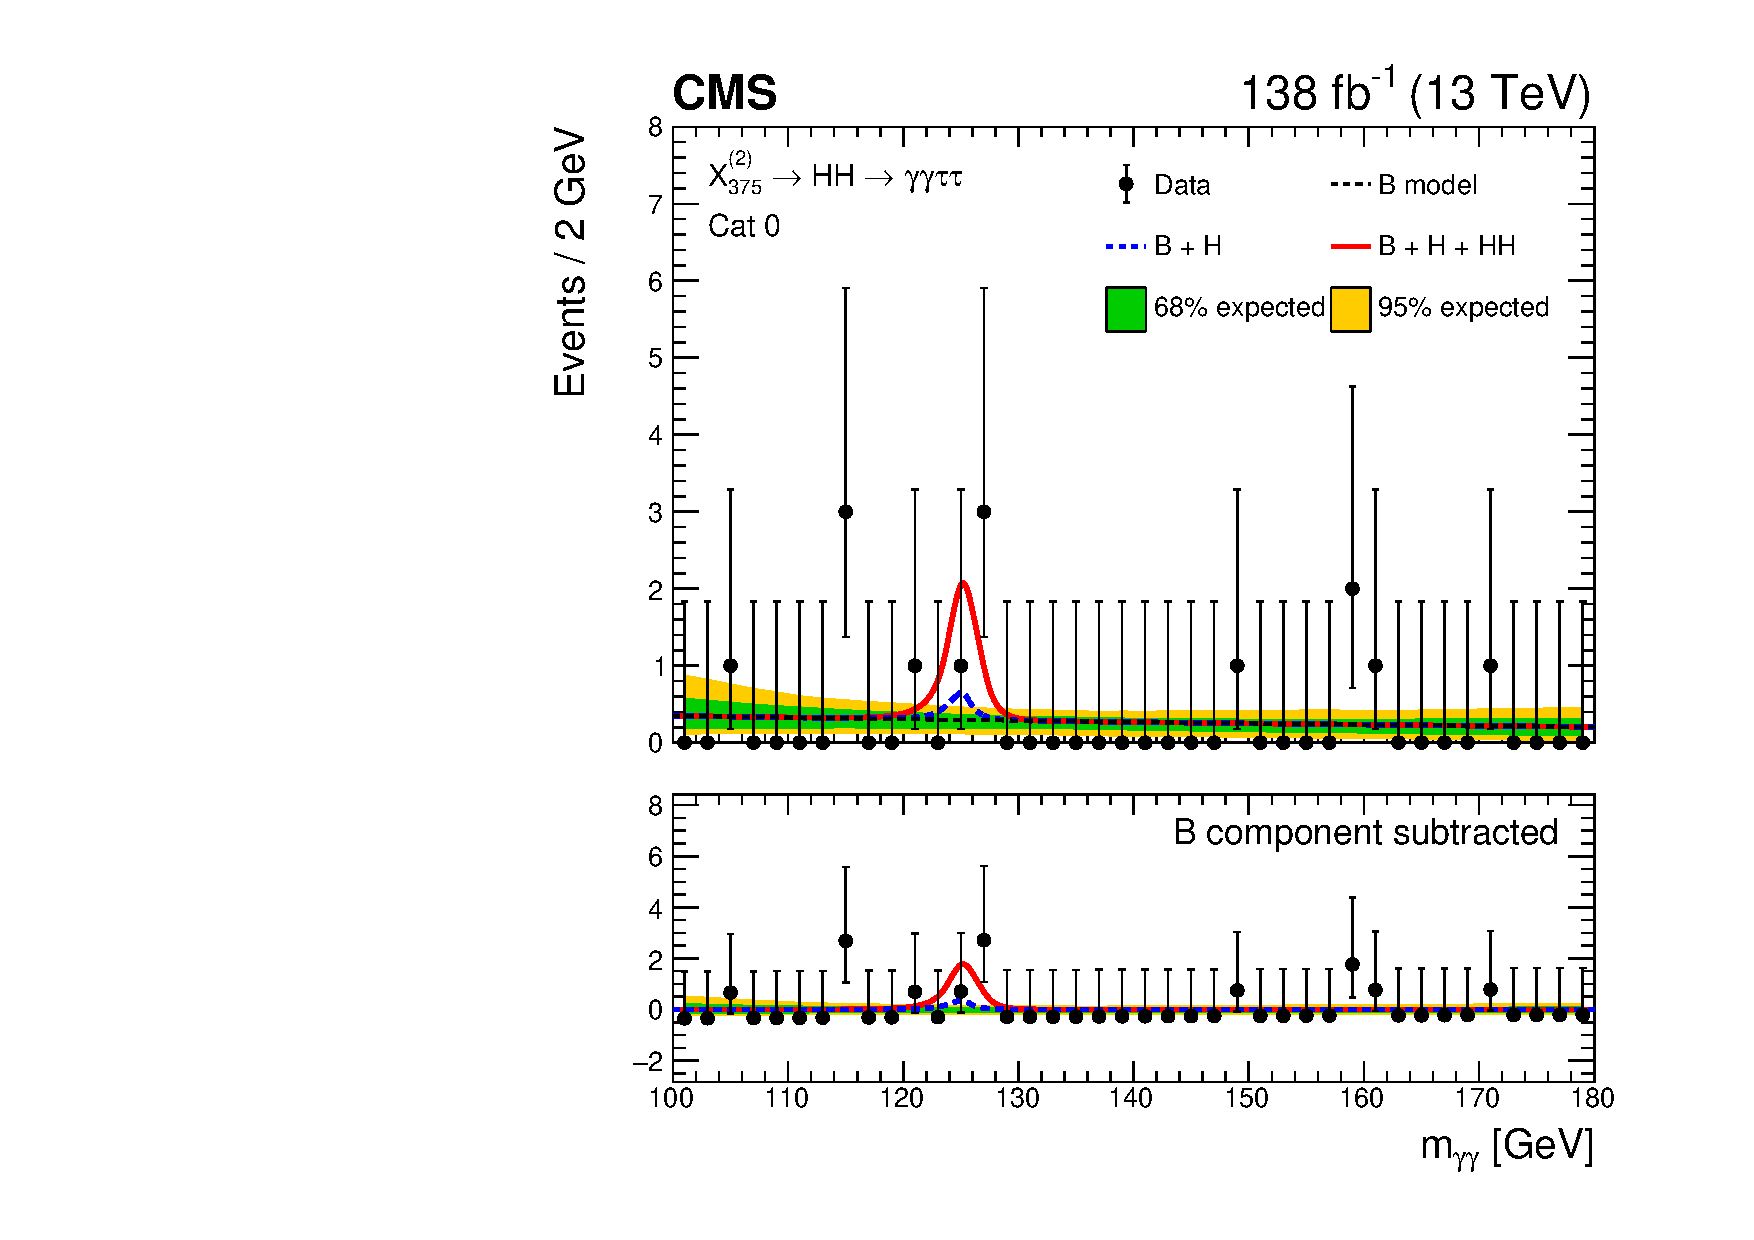
\includegraphics[width=.45\linewidth]{Figures/Dihiggs/results/sb_models/graviton/ARCGL_Graviton_mx375my125_ggttresmx375my125cat0_CMS_hgg_mass_nbins40_paper.pdf}
    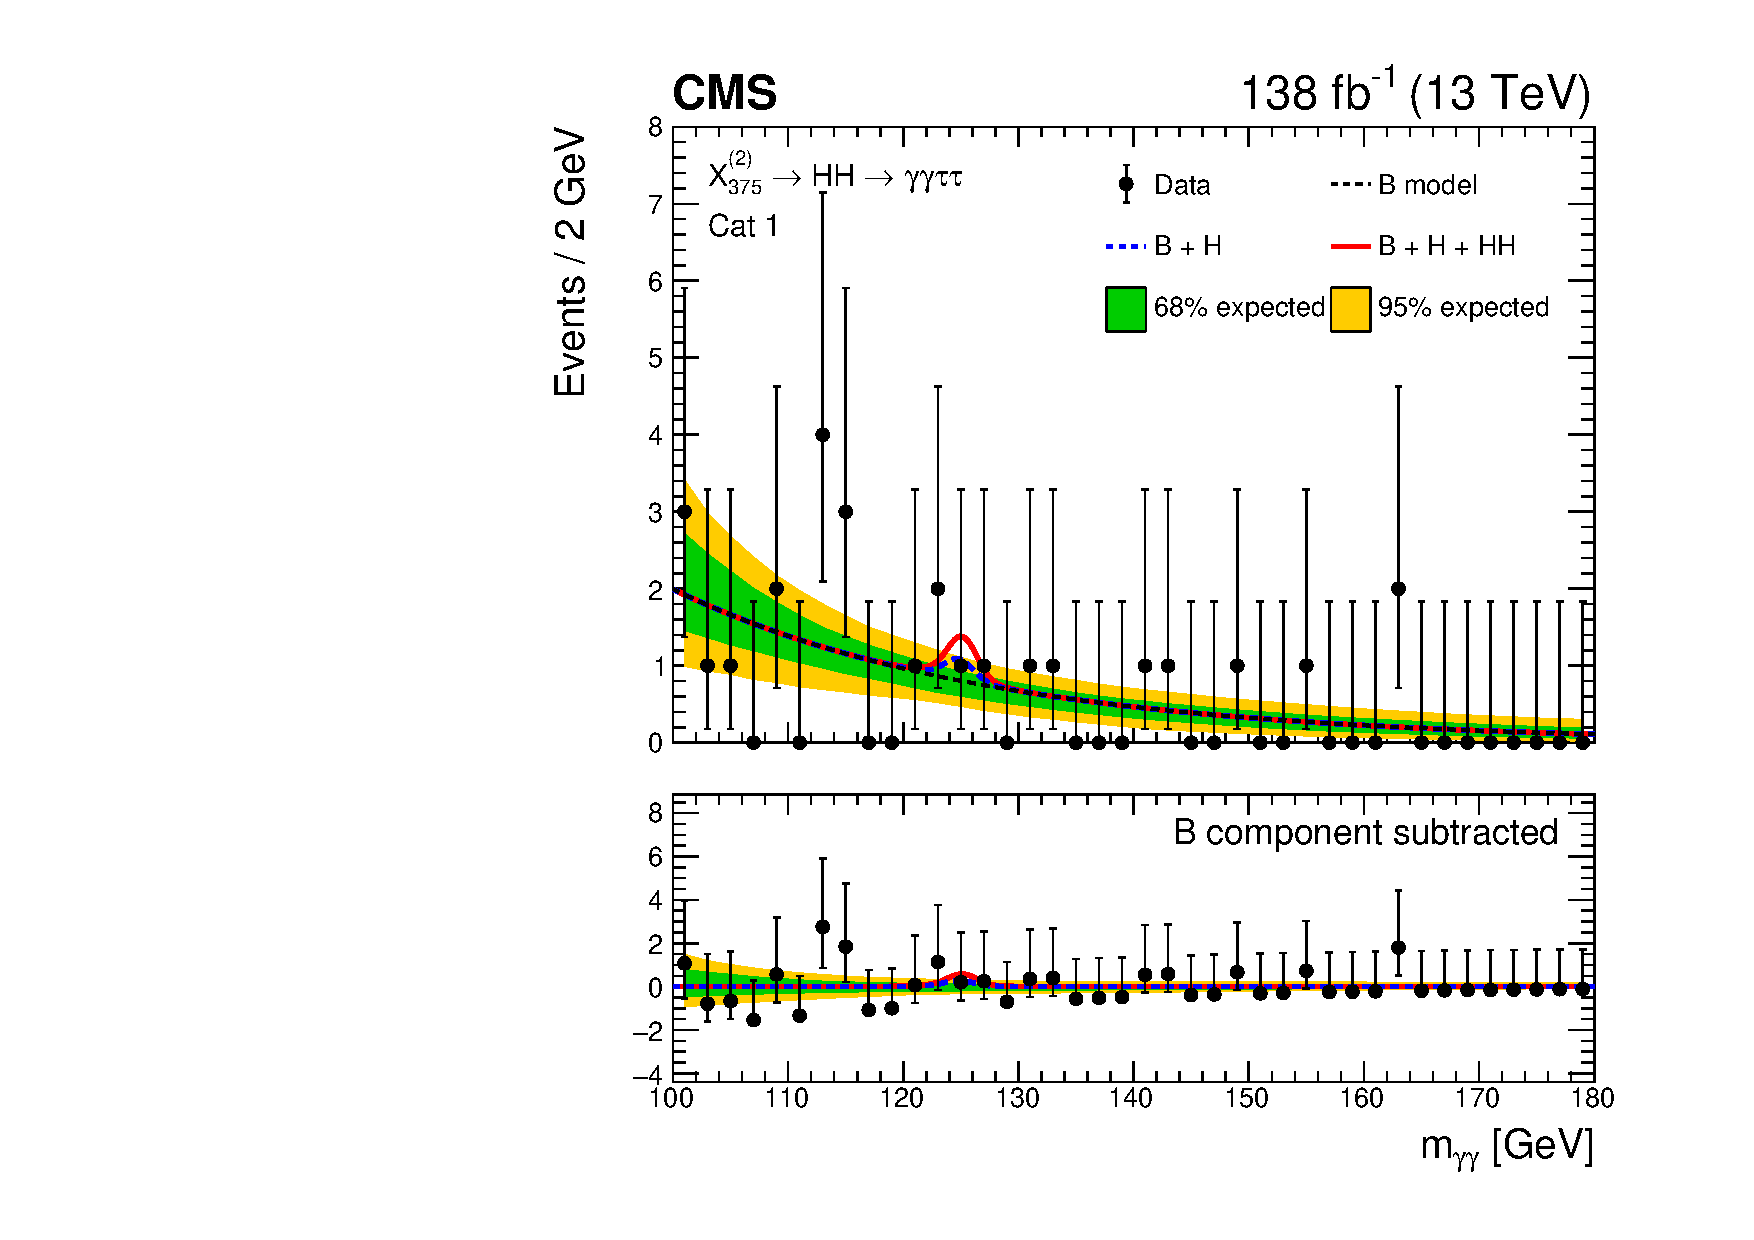
\includegraphics[width=.45\linewidth]{Figures/Dihiggs/results/sb_models/graviton/ARCGL_Graviton_mx375my125_ggttresmx375my125cat1_CMS_hgg_mass_nbins40_paper.pdf}
    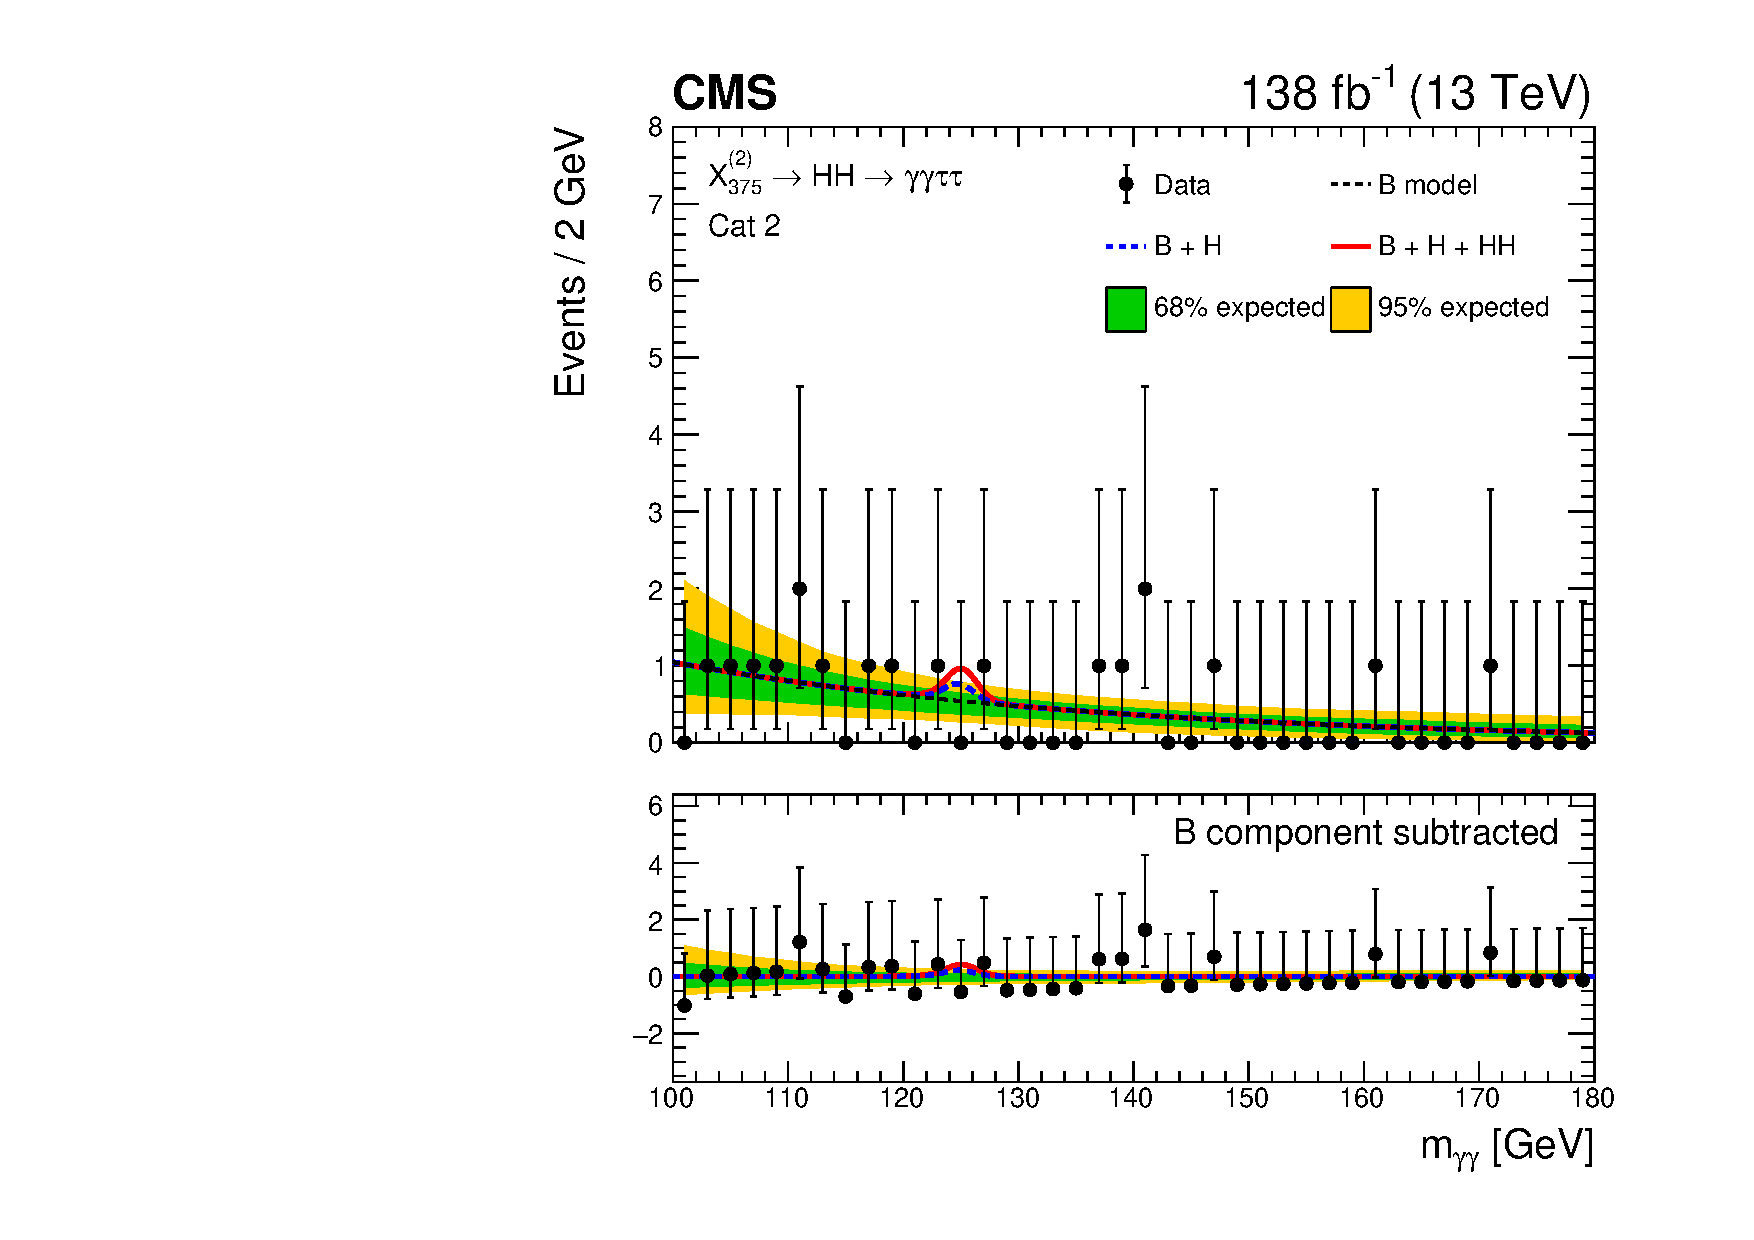
\includegraphics[width=.45\linewidth]{Figures/Dihiggs/results/sb_models/graviton/ARCGL_Graviton_mx375my125_ggttresmx375my125cat2_CMS_hgg_mass_nbins40_paper.pdf}
    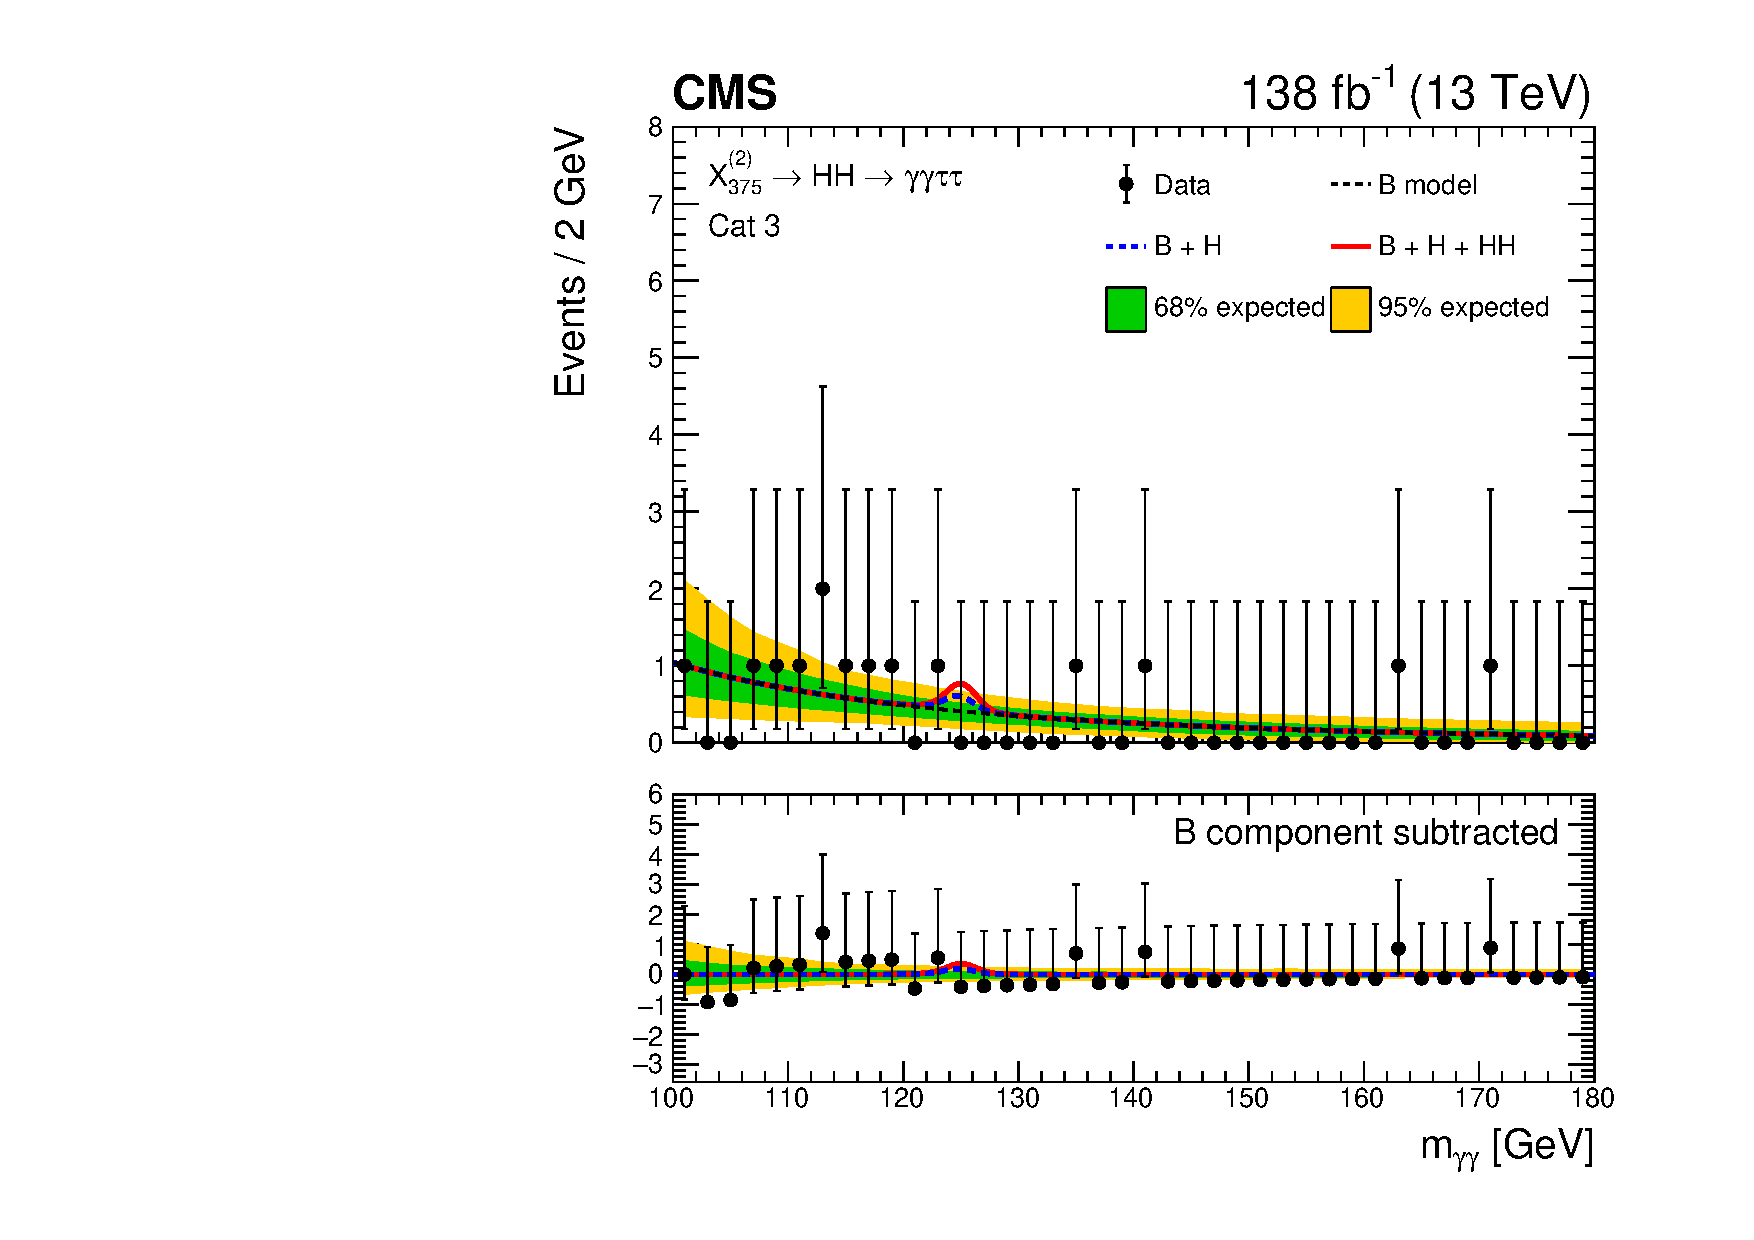
\includegraphics[width=.45\linewidth]{Figures/Dihiggs/results/sb_models/graviton/ARCGL_Graviton_mx375my125_ggttresmx375my125cat3_CMS_hgg_mass_nbins40_paper.pdf}
    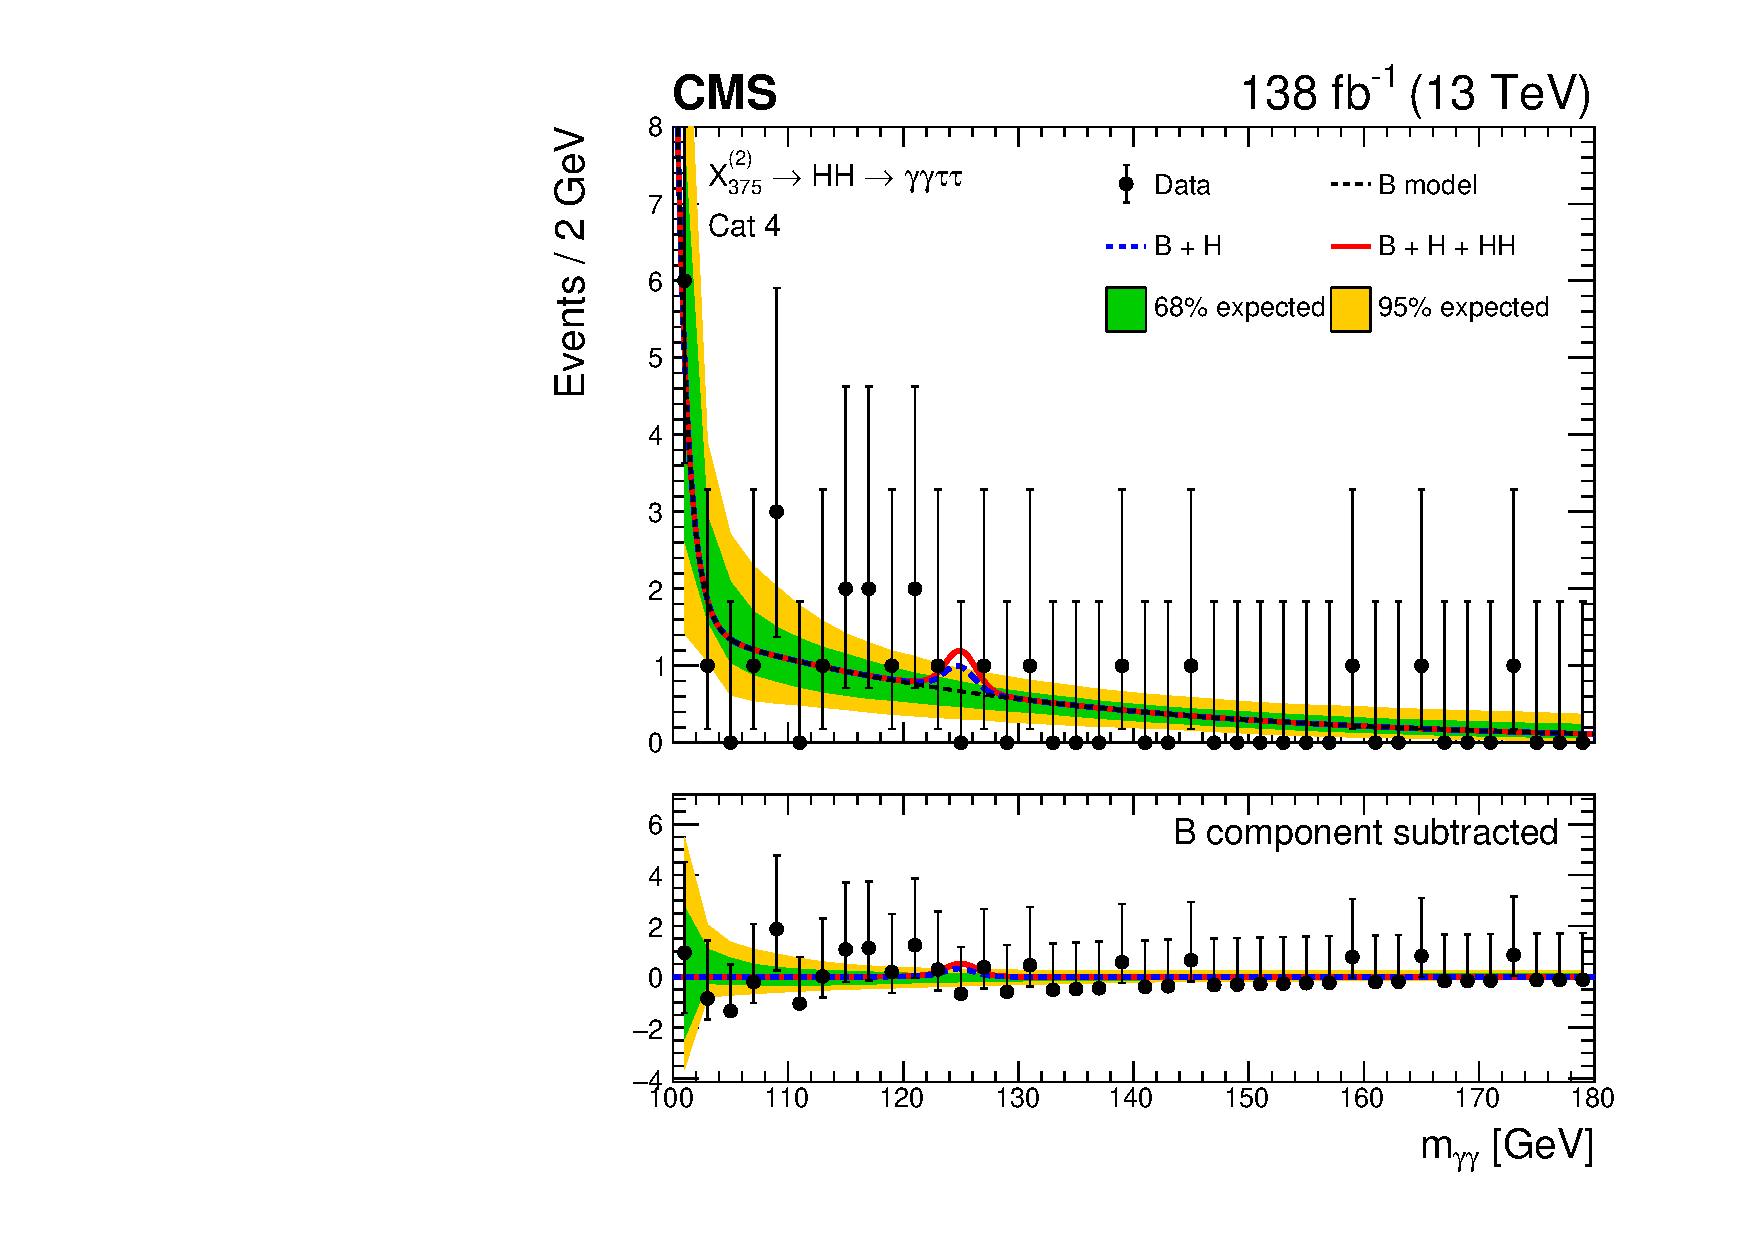
\includegraphics[width=.45\linewidth]{Figures/Dihiggs/results/sb_models/graviton/ARCGL_Graviton_mx375my125_ggttresmx375my125cat4_CMS_hgg_mass_nbins40_paper.pdf}
    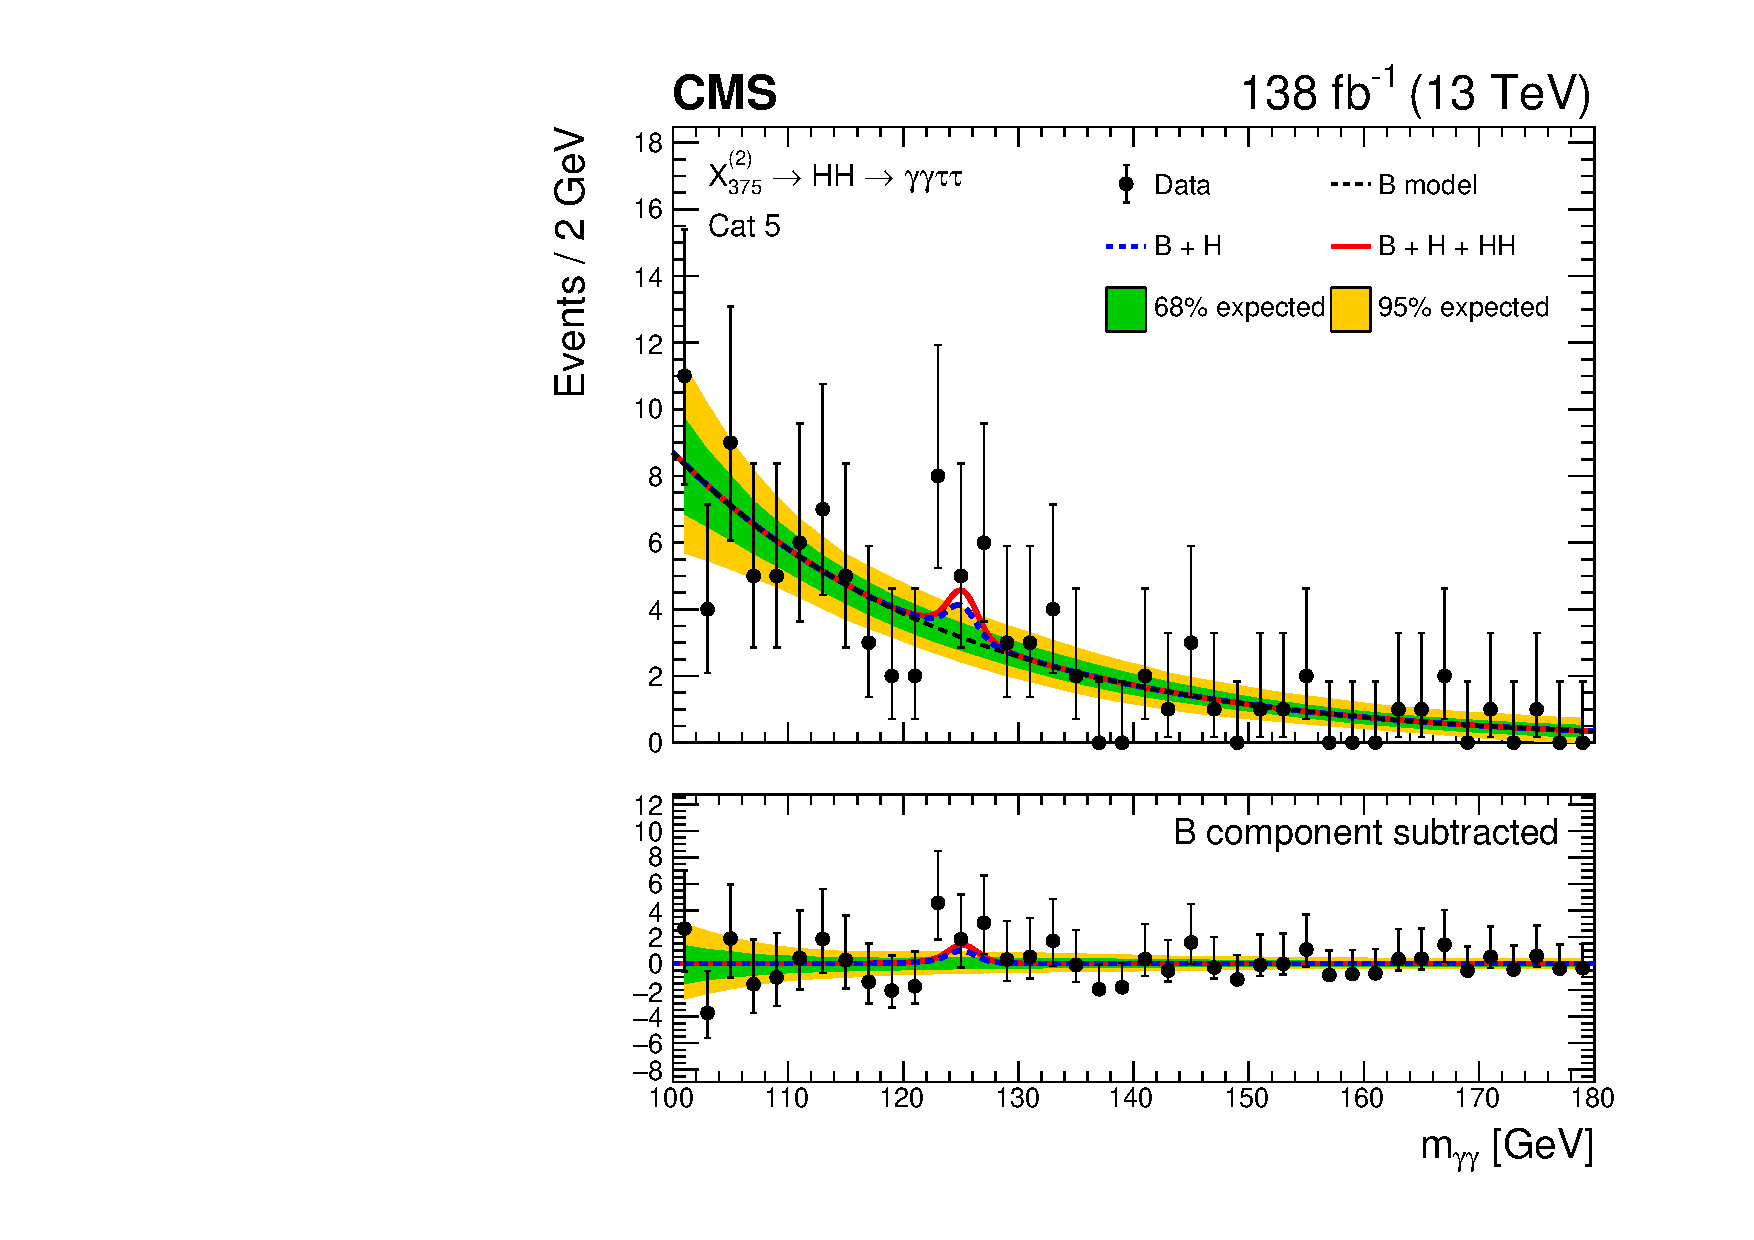
\includegraphics[width=.45\linewidth]{Figures/Dihiggs/results/sb_models/graviton/ARCGL_Graviton_mx375my125_ggttresmx375my125cat5_CMS_hgg_mass_nbins40_paper.pdf}
    \caption[Signal-Plus-Background Fits to Data for \XTwoHH Search at $\mX=375$\GeV]{Distributions of \mgg in data in each analysis category and the signal-plus-background models (red) with data (black points) for the mass hypothesis with the largest excess in the \XTwoHH search: $\mX=$~375\GeV. The one (green) standard deviation and two (yellow) standard deviation bands show the uncertainties in the nonresonant background component of the model (black dashed line). The resonant single-Higgs background is plotted separately in blue (blue dashed line). The lower panel shows the residuals after subtraction of the nonresonant background component.}\label{fig:sbmodel_1}
\end{figure}

The expected and observed 95\% CL upper limits on $\sigma(\ppXHH)$ for the \XZeroHH and \XTwoHH searches are shown in \cref{fig:limits_xhh}. The limits are found to decrease as a function of \mX, which is expected given the higher preselection signal efficiency and better signal-to-background discrimination seen at higher masses. The observed (expected) upper limits vary between 160--2200\fb (240--1800\fb) and 180--1900\fb (200--1800\fb) for the \XZeroHH and \XTwoHH searches respectively. Interpreting these results in the RS bulk model (\cref{sec:wed}), a spin-0 Radion resonance with mass of up to 550\GeV is excluded when $\Lambda_R=3$\TeV, or up to 900\GeV is excluded when $\Lambda_R=2$\TeV. For the spin-2 KK Graviton, a resonance with a mass between 310 and 700\GeV is excluded when assuming $\tilde{\kappa} = 1$.

\begin{figure}
    \centering
    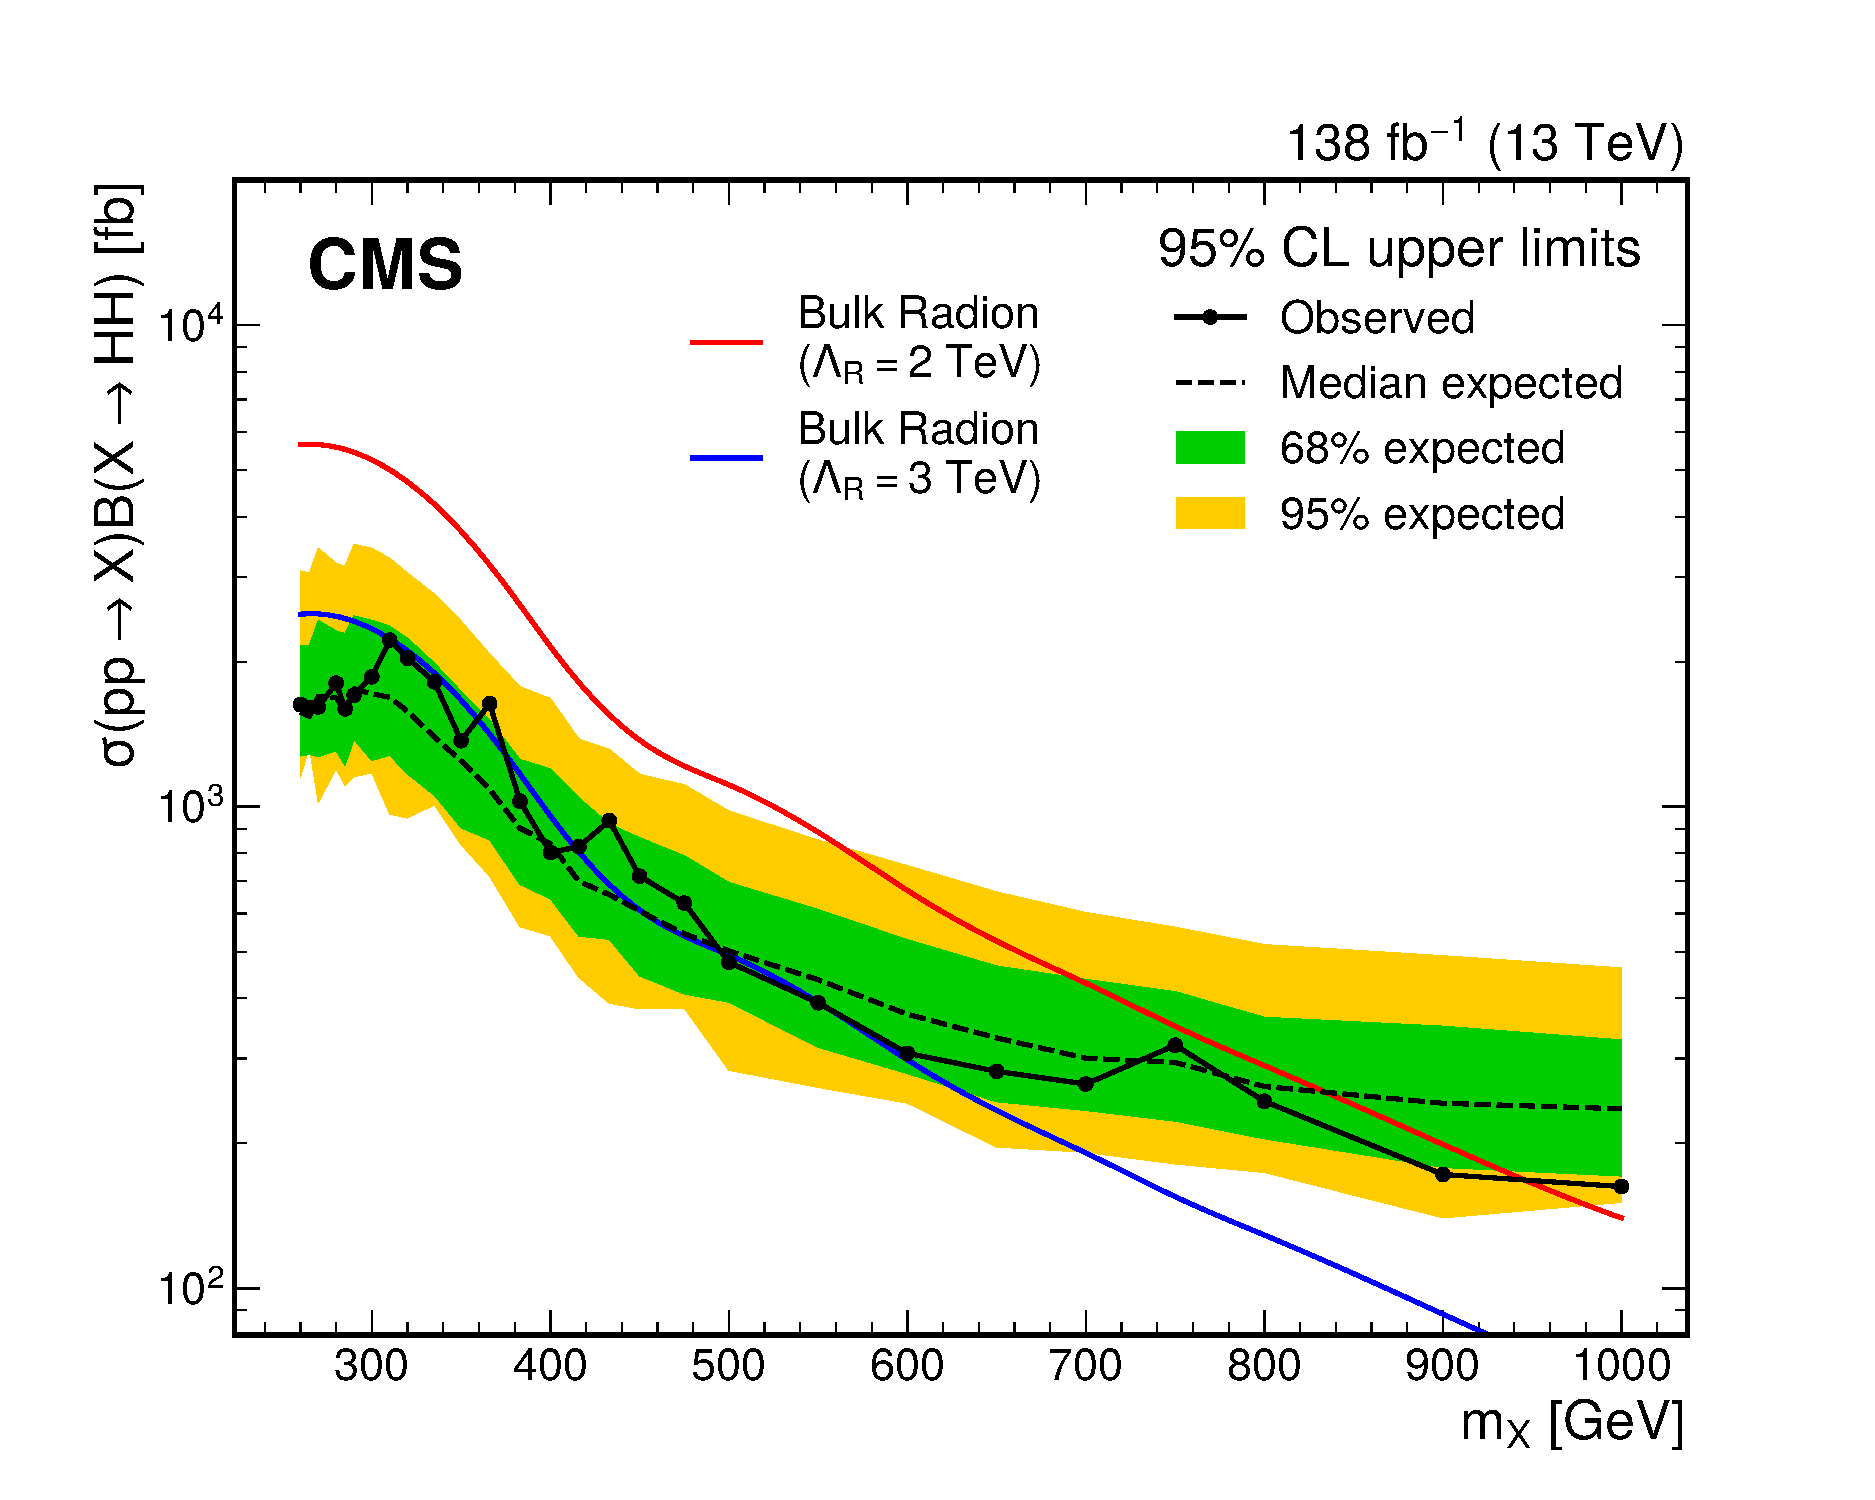
\includegraphics[width=0.8\textwidth]{Figures/Dihiggs/results/limits/limits_radion_paper.pdf}
    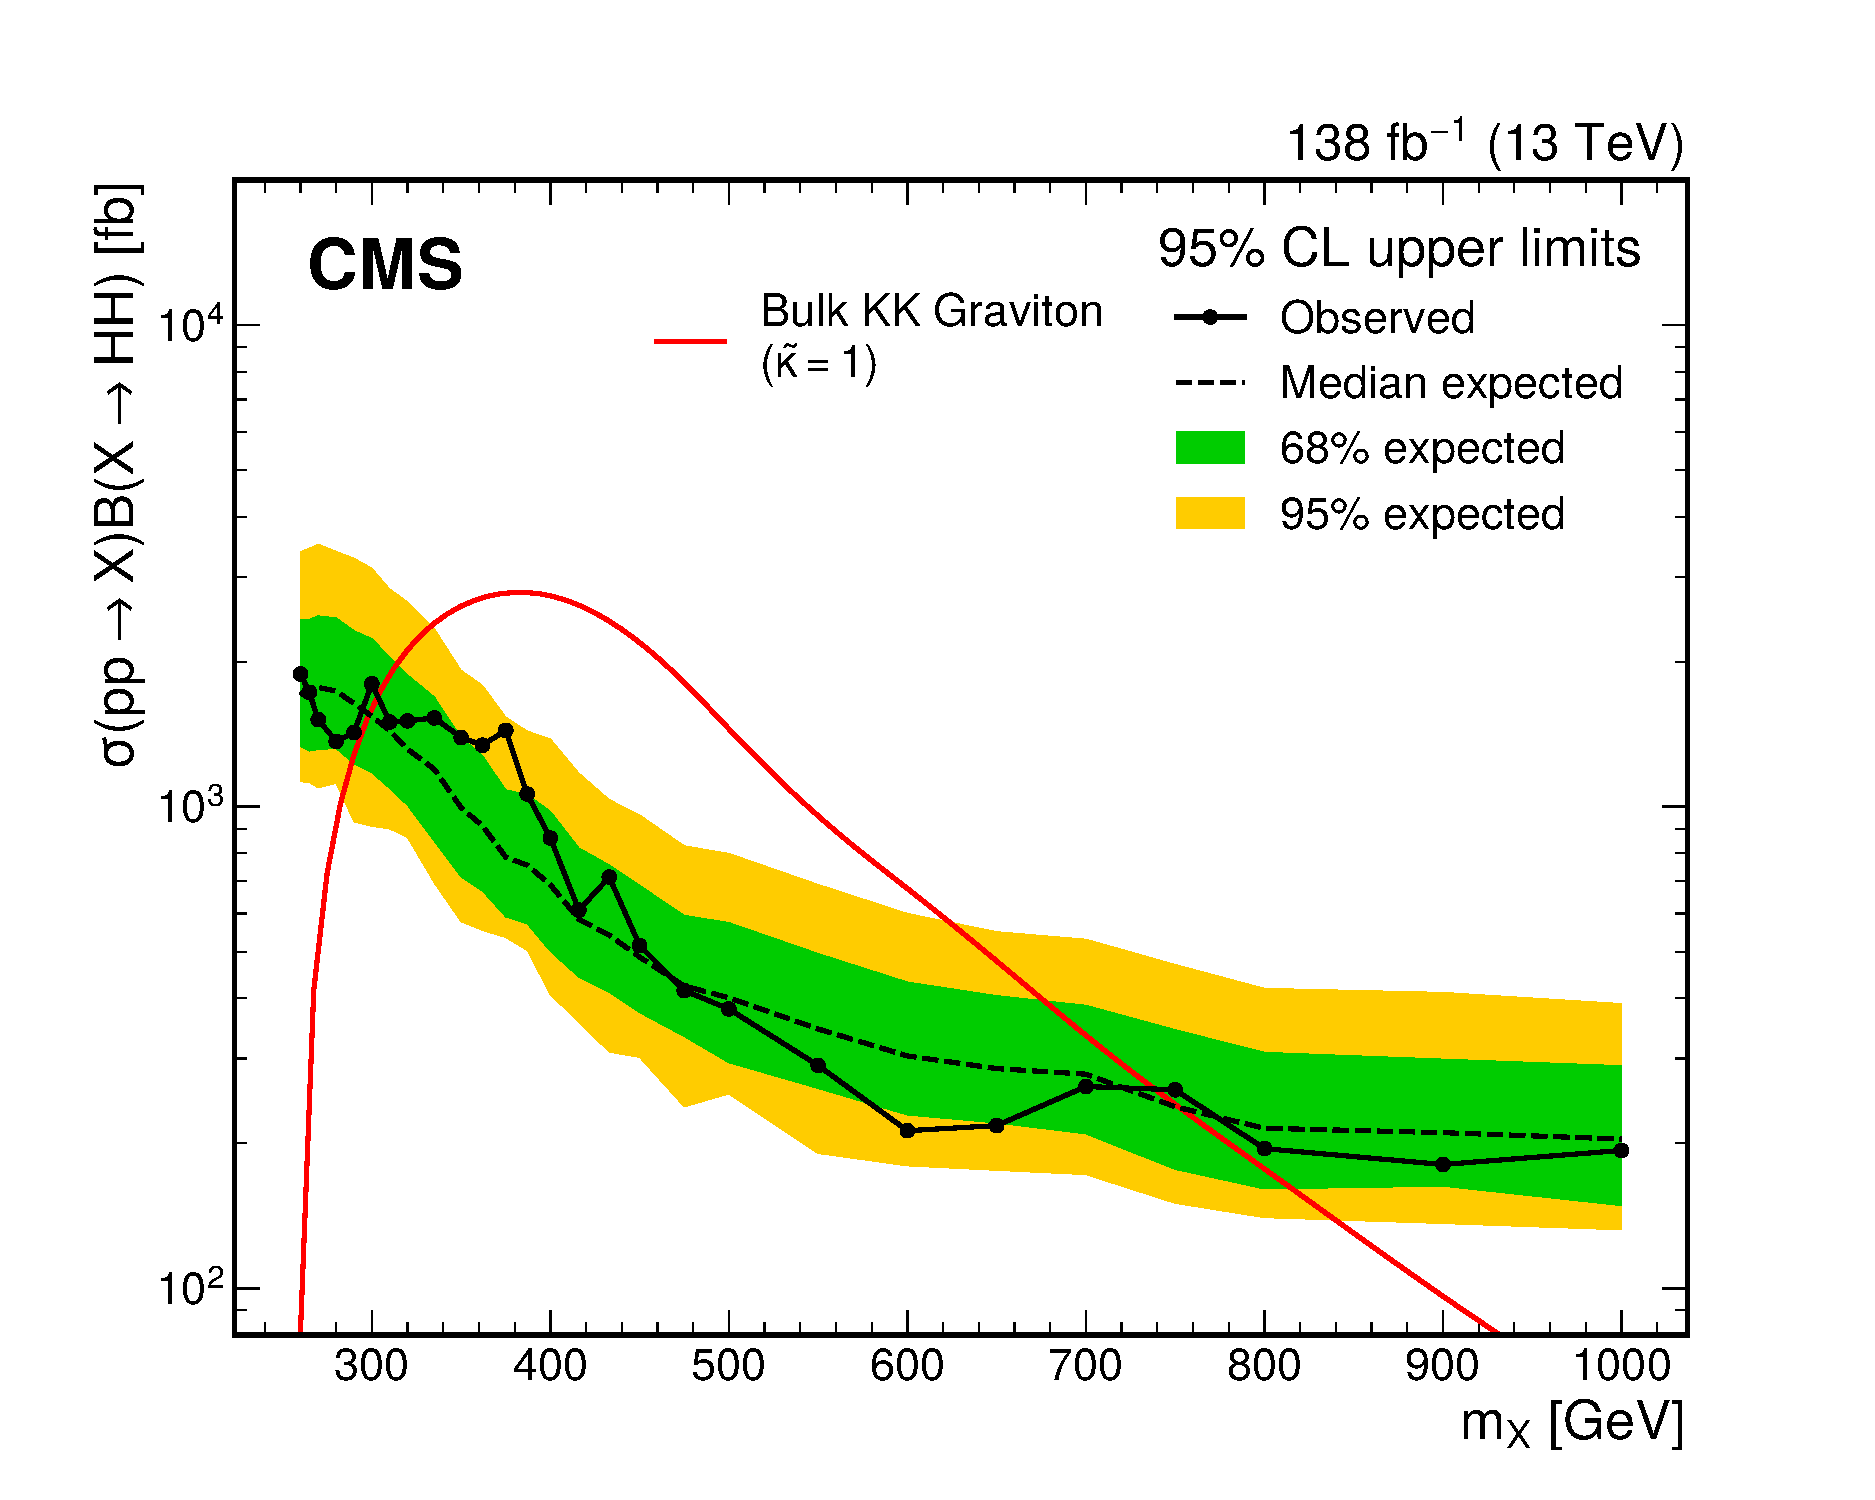
\includegraphics[width=0.8\textwidth]{Figures/Dihiggs/results/limits/limits_graviton_paper.pdf}
    \caption[\XHH Upper Limits]{Expected and observed 95\% CL upper limits on $\sigma(\ppXHH)$ for the \XZeroHH (top) and \XTwoHH (bottom) searches. The solid and dashed black lines represent observed and median expected limits respectively. The inner (green) band and the outer (yellow) band indicate the regions containing 68 and 95\%, respectively, of the distribution of limits expected under the background-only hypothesis. The red and blue lines show WED theory predictions at values of the theory parameters specified in the legend.}\label{fig:limits_xhh}
\end{figure}

In an analogous search performed by the CMS experiment in the \bbgg final state~\cite{CMS:2023boe}, the observed upper limits on $\sigma(\ppXHH)$ were found to be about 26--310\fb and 23--290\fb for the \XZeroHH and \XTwoHH searches respectively. Therefore, the \ggtt final state does not provide the most competitive results in the \XHH searches, but this was expected given the smaller branching fraction of \Htautau relative to \Hbb. Nonetheless, the \ggtt final state can be used in a future combination of final states that should provide a sensitivity greater than any final state alone. In the \XYH searches, which are discussed in the rest of this section, the branching fractions of the \PY scalar are unspecified and therefore, these searches can yield interesting standalone results. 

\subsection[\texorpdfstring{\XYttHgg}{XY(gg)H(tt)} Search]{\XYttHgg Search}\label{sec:results_y_tautau}

\Cref{fig:significance_y_tautau} shows the local significances for every mass point in the \XYttHgg search. Local significances of about 2 standard deviations can be seen for a band in $\mX$ and $\mY$ that stretches between $\mX=300$ and 500\GeV and for values of $(\mX-\mY)\approx200$\GeV. The largest excess is seen at $(\mX,\mY)=(320,60)$\GeV with a local (global) significance of 2.6 (2.2) standard deviations. The \mgg distributions in data for this mass point, and the corresponding signal-plus-background model fit, is shown in \cref{fig:sbmodel_2}. Looking at these figures, the excess seems to driven primarily by the 6 events in the interval $120 < \mgg < 130$\GeV in category 0, although there are also noticeable, albeit smaller, excesses in categories 3 and 5.

\begin{figure}
    \centering
    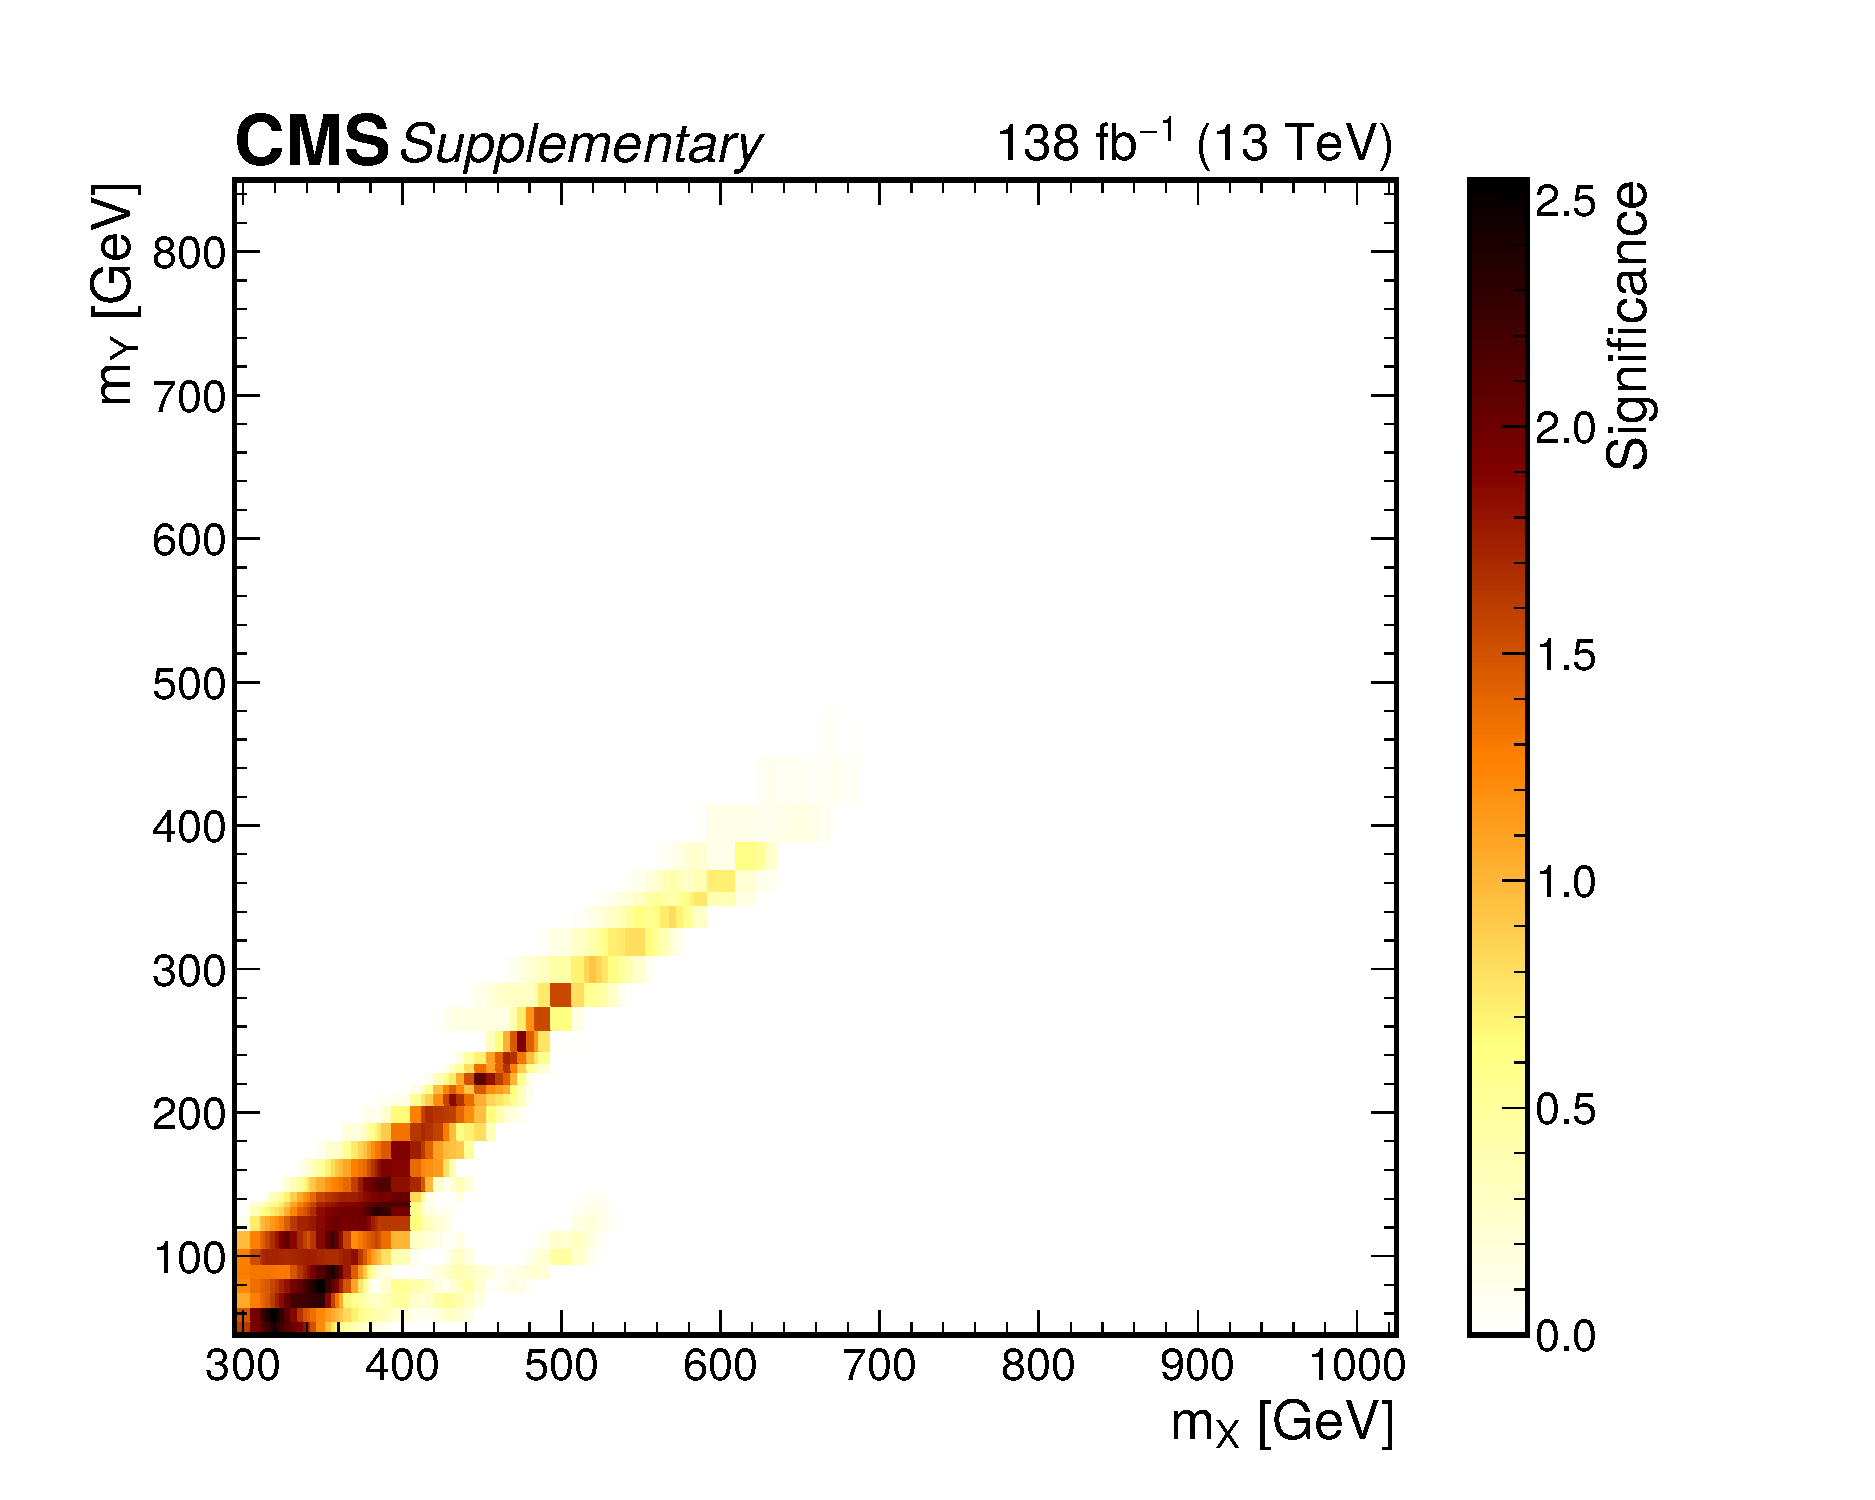
\includegraphics[width=0.8\textwidth]{Figures/Dihiggs/results/significances/significance_y_tautau_supplementary.pdf}
    \caption[\XYttHgg Observed Local Significances]{Observed local significances in the 2D $(\mX,\mY)$ plane for the \XYttHgg search.}\label{fig:significance_y_tautau}
\end{figure}

\begin{figure}
    \centering
    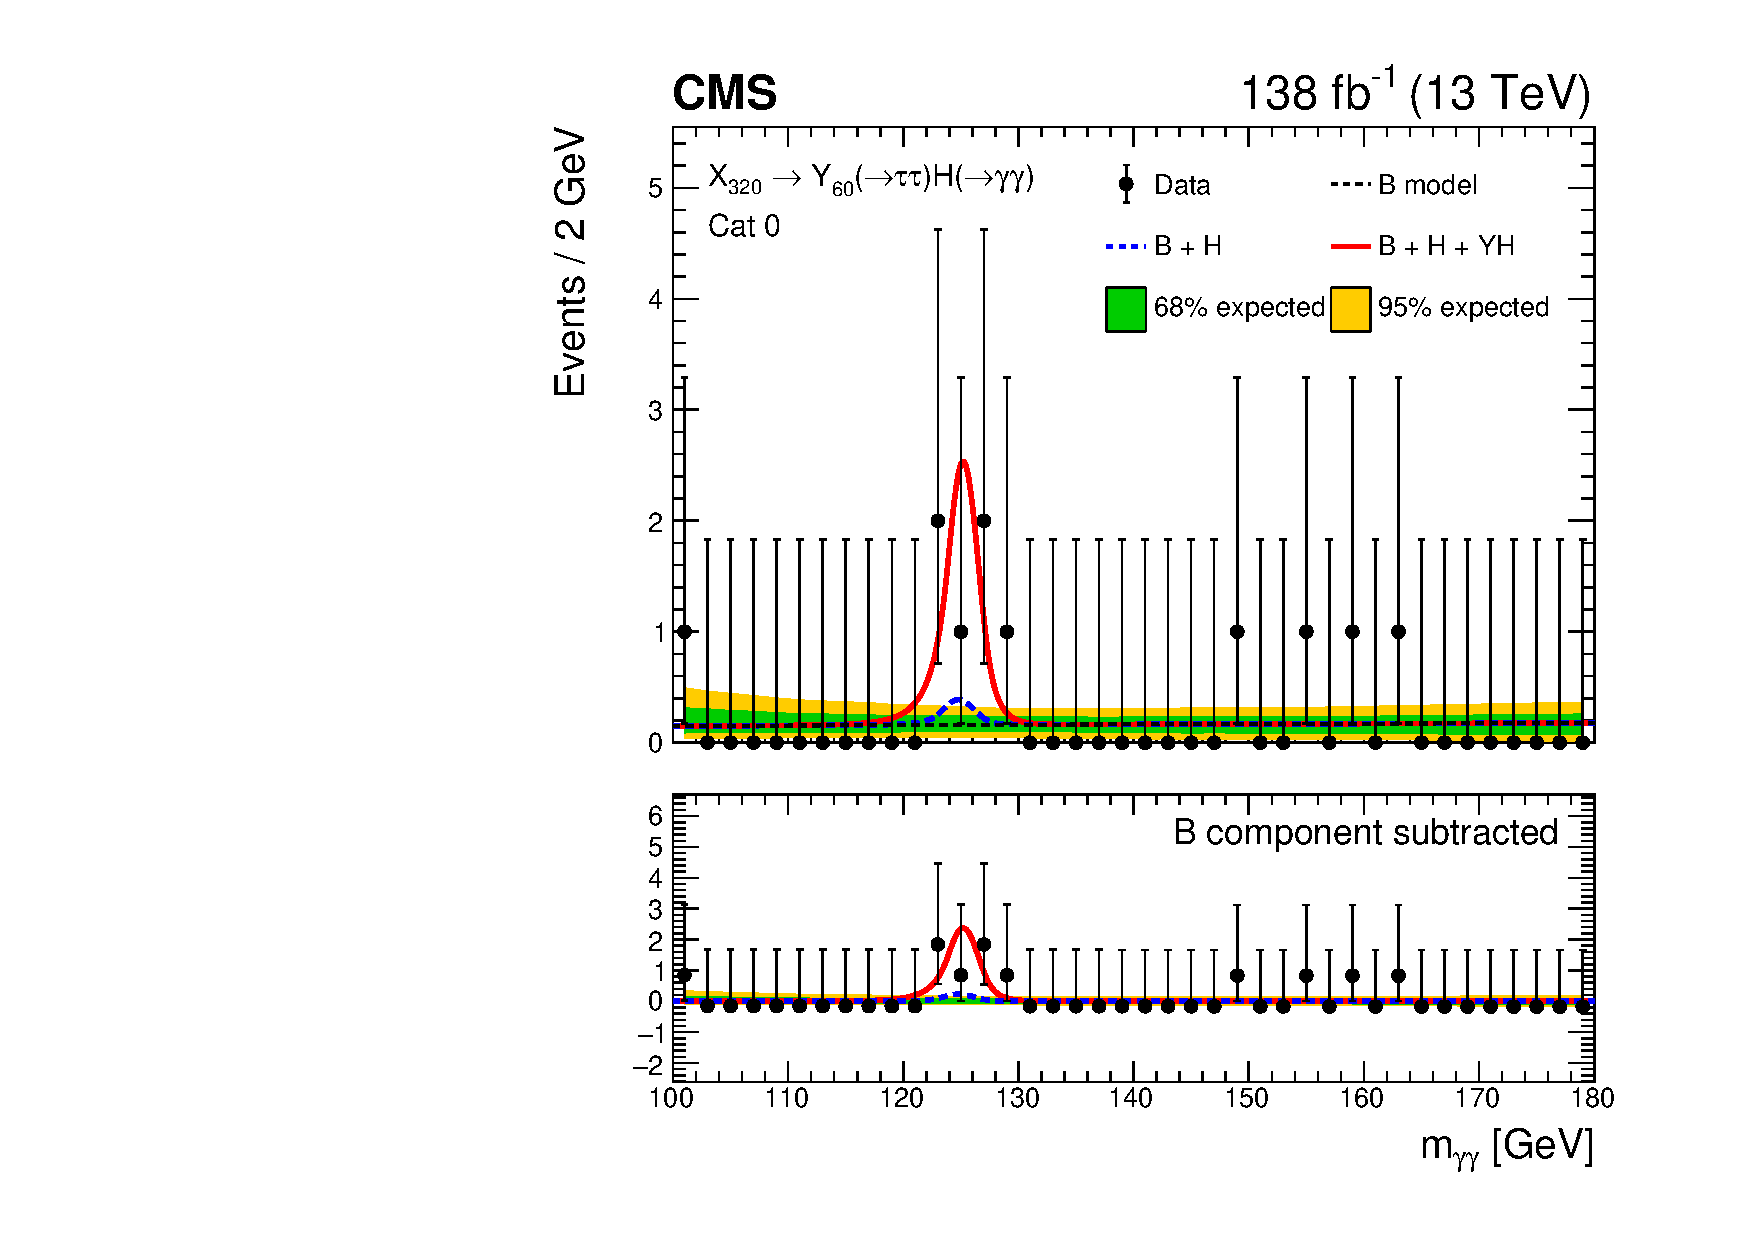
\includegraphics[width=.45\linewidth]{Figures/Dihiggs/results/sb_models/y_tautau/ARCGL_Y_tautau_mx320my60_ggttresmx320my60cat0_CMS_hgg_mass_nbins40_paper.pdf}
    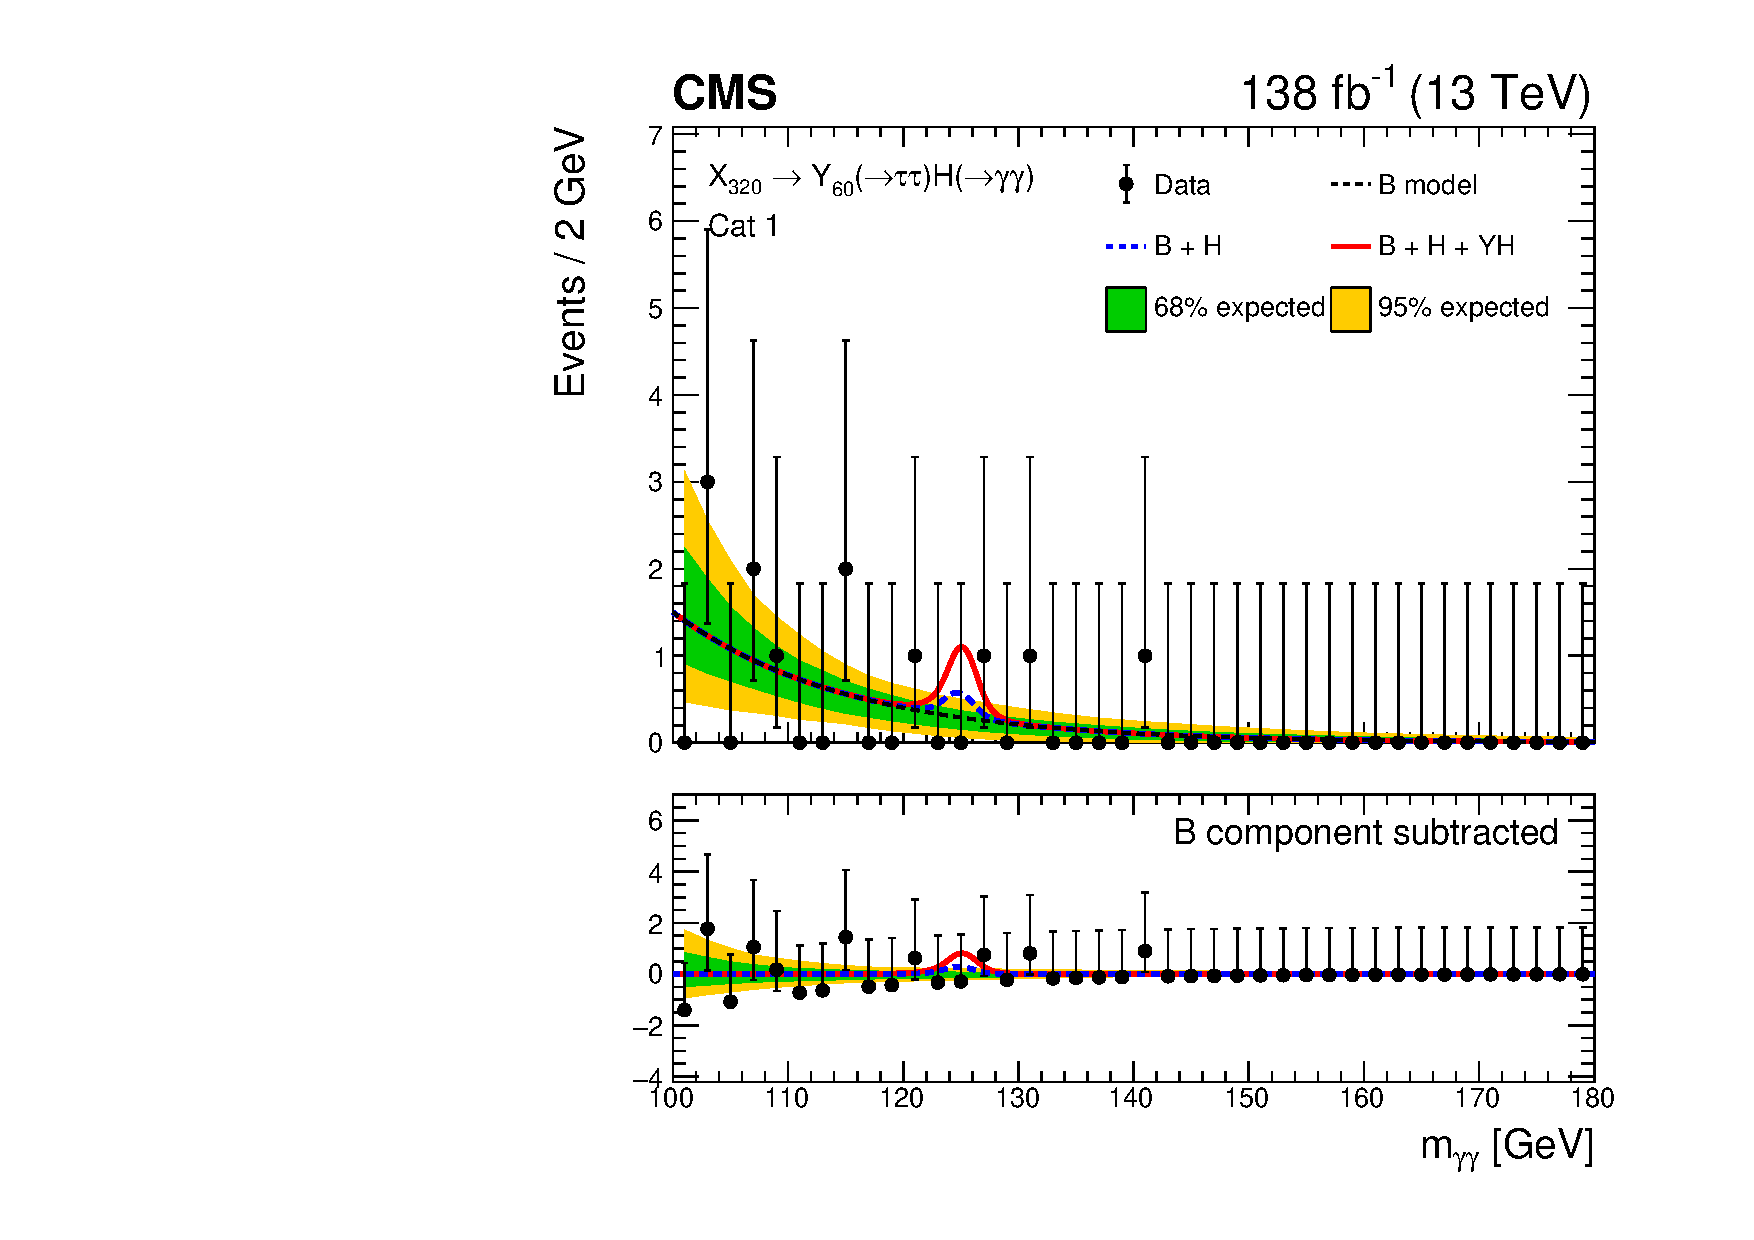
\includegraphics[width=.45\linewidth]{Figures/Dihiggs/results/sb_models/y_tautau/ARCGL_Y_tautau_mx320my60_ggttresmx320my60cat1_CMS_hgg_mass_nbins40_paper.pdf}
    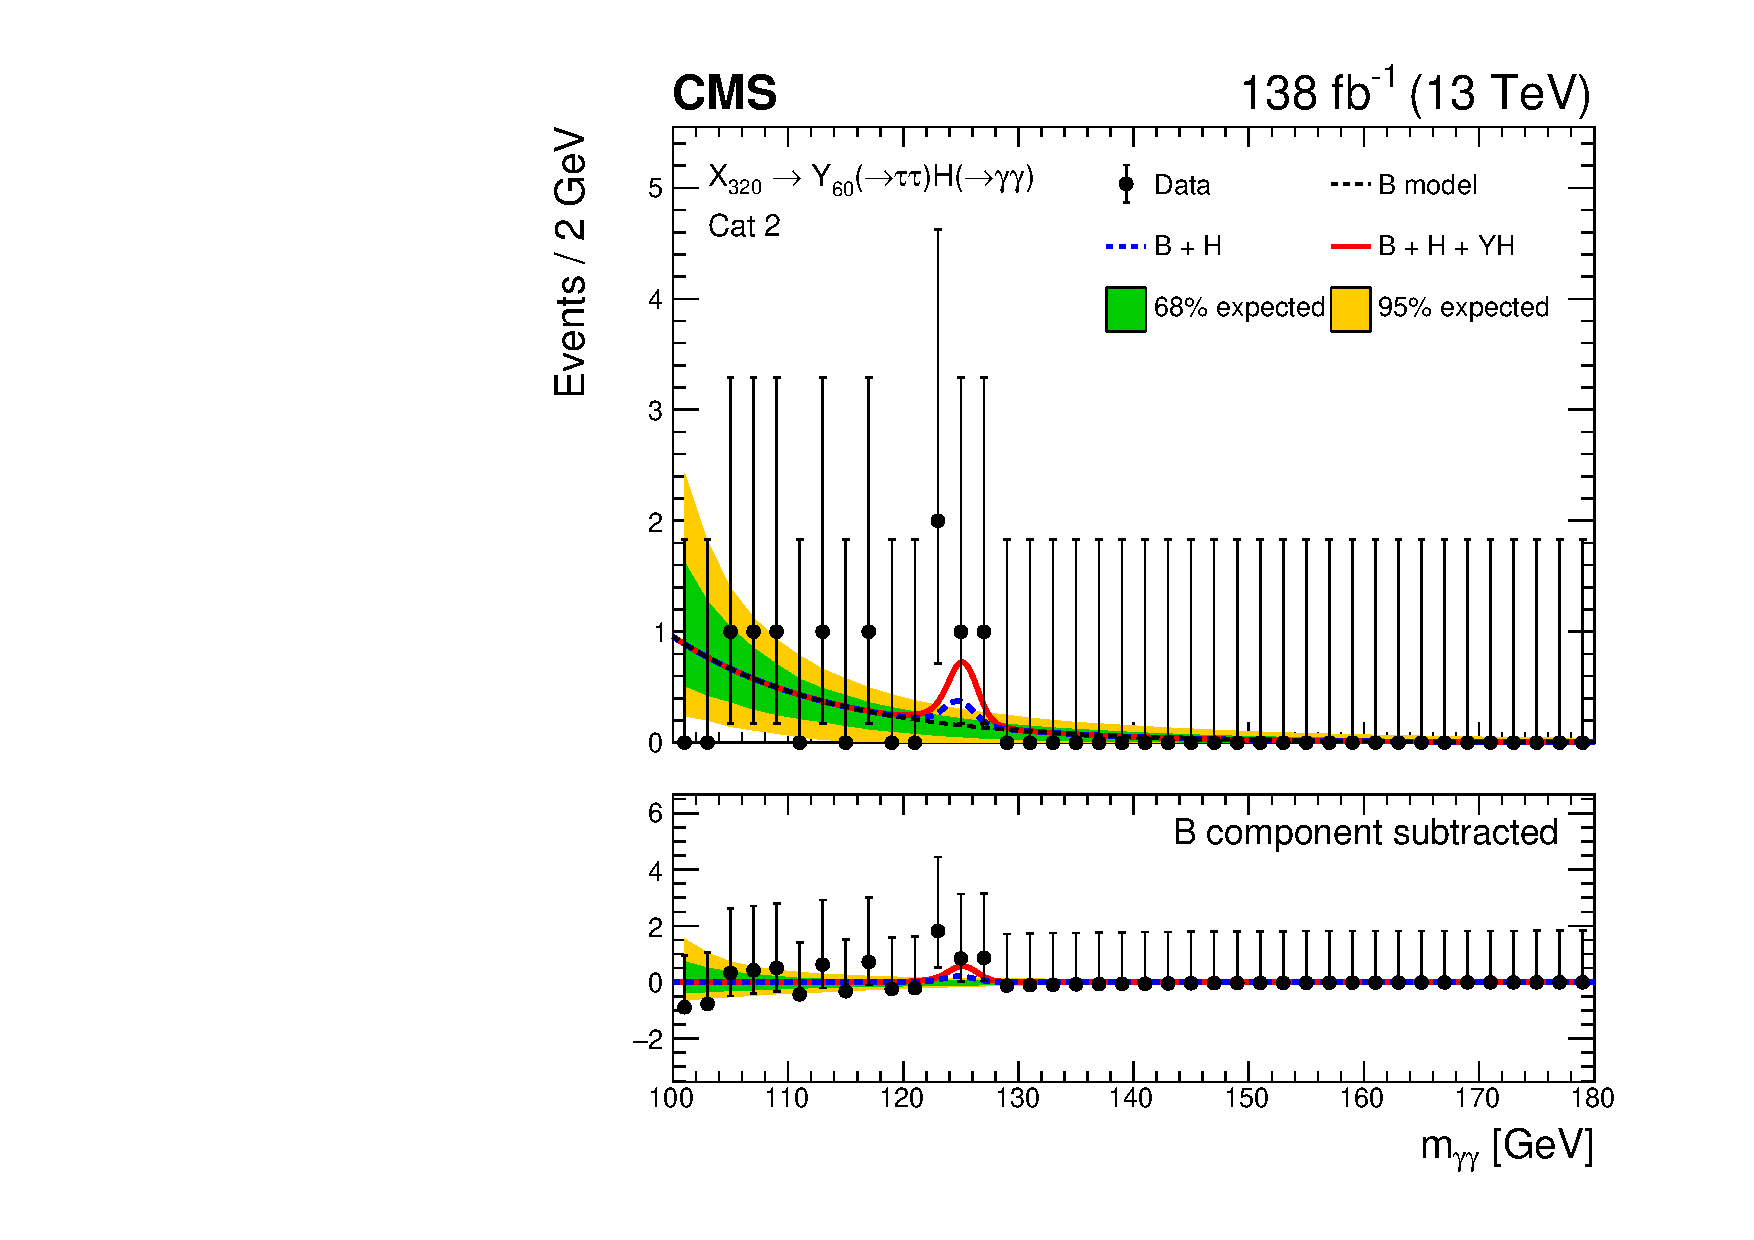
\includegraphics[width=.45\linewidth]{Figures/Dihiggs/results/sb_models/y_tautau/ARCGL_Y_tautau_mx320my60_ggttresmx320my60cat2_CMS_hgg_mass_nbins40_paper.pdf}
    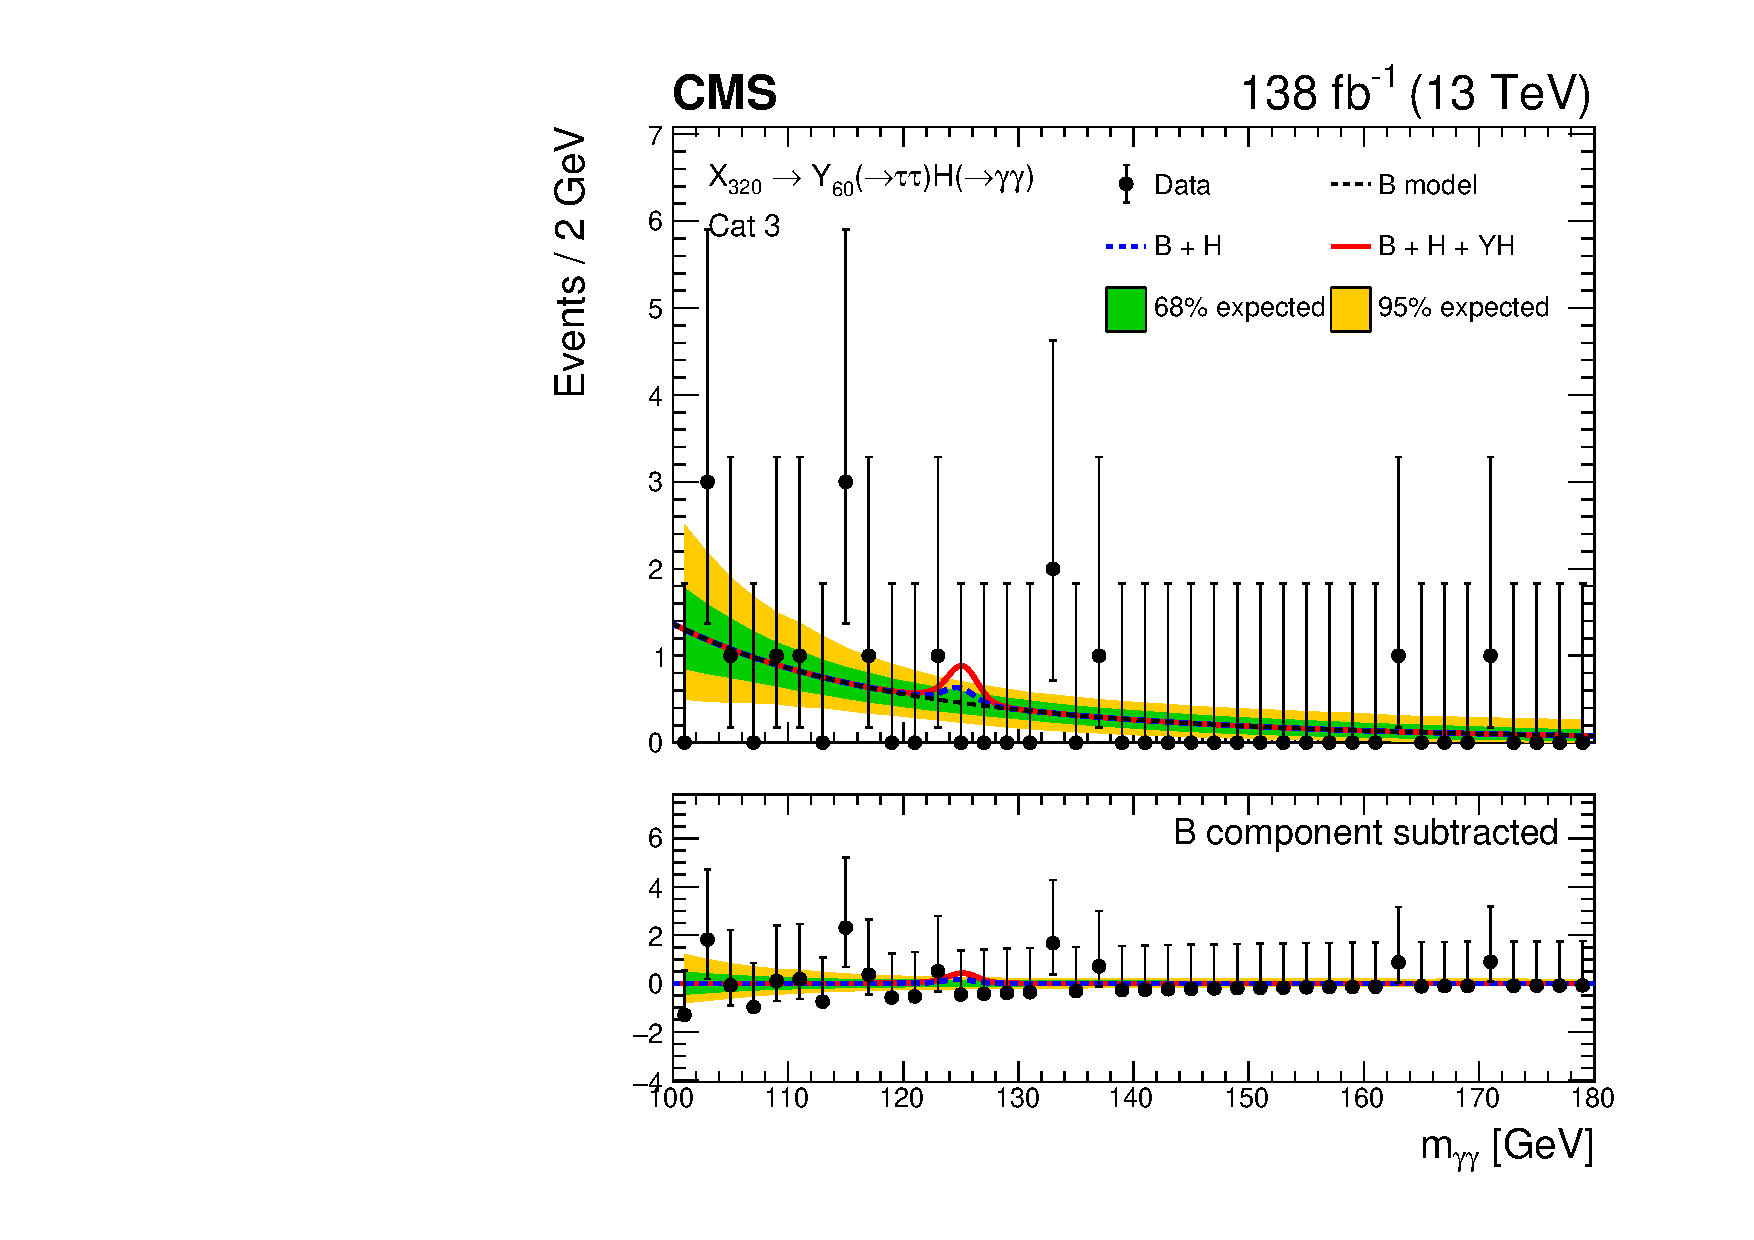
\includegraphics[width=.45\linewidth]{Figures/Dihiggs/results/sb_models/y_tautau/ARCGL_Y_tautau_mx320my60_ggttresmx320my60cat3_CMS_hgg_mass_nbins40_paper.pdf}
    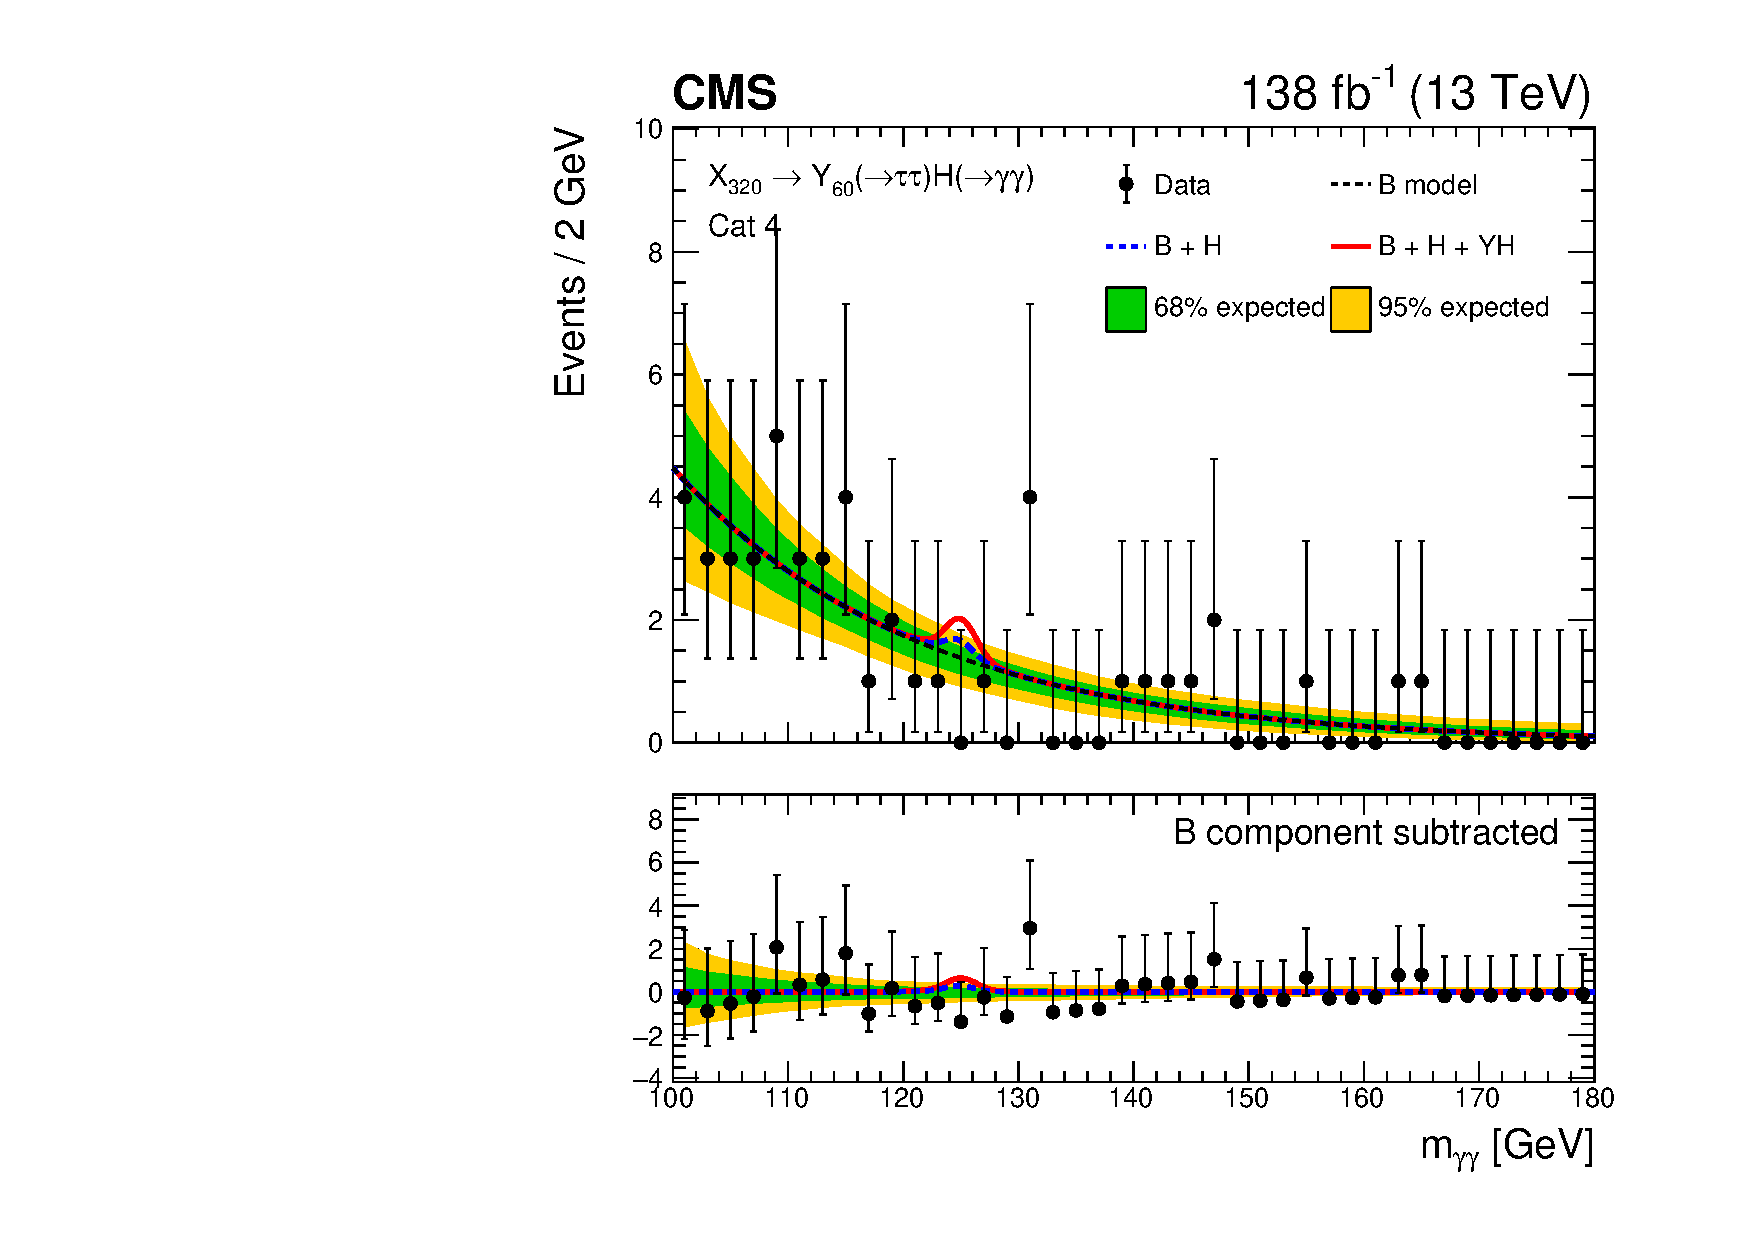
\includegraphics[width=.45\linewidth]{Figures/Dihiggs/results/sb_models/y_tautau/ARCGL_Y_tautau_mx320my60_ggttresmx320my60cat4_CMS_hgg_mass_nbins40_paper.pdf}
    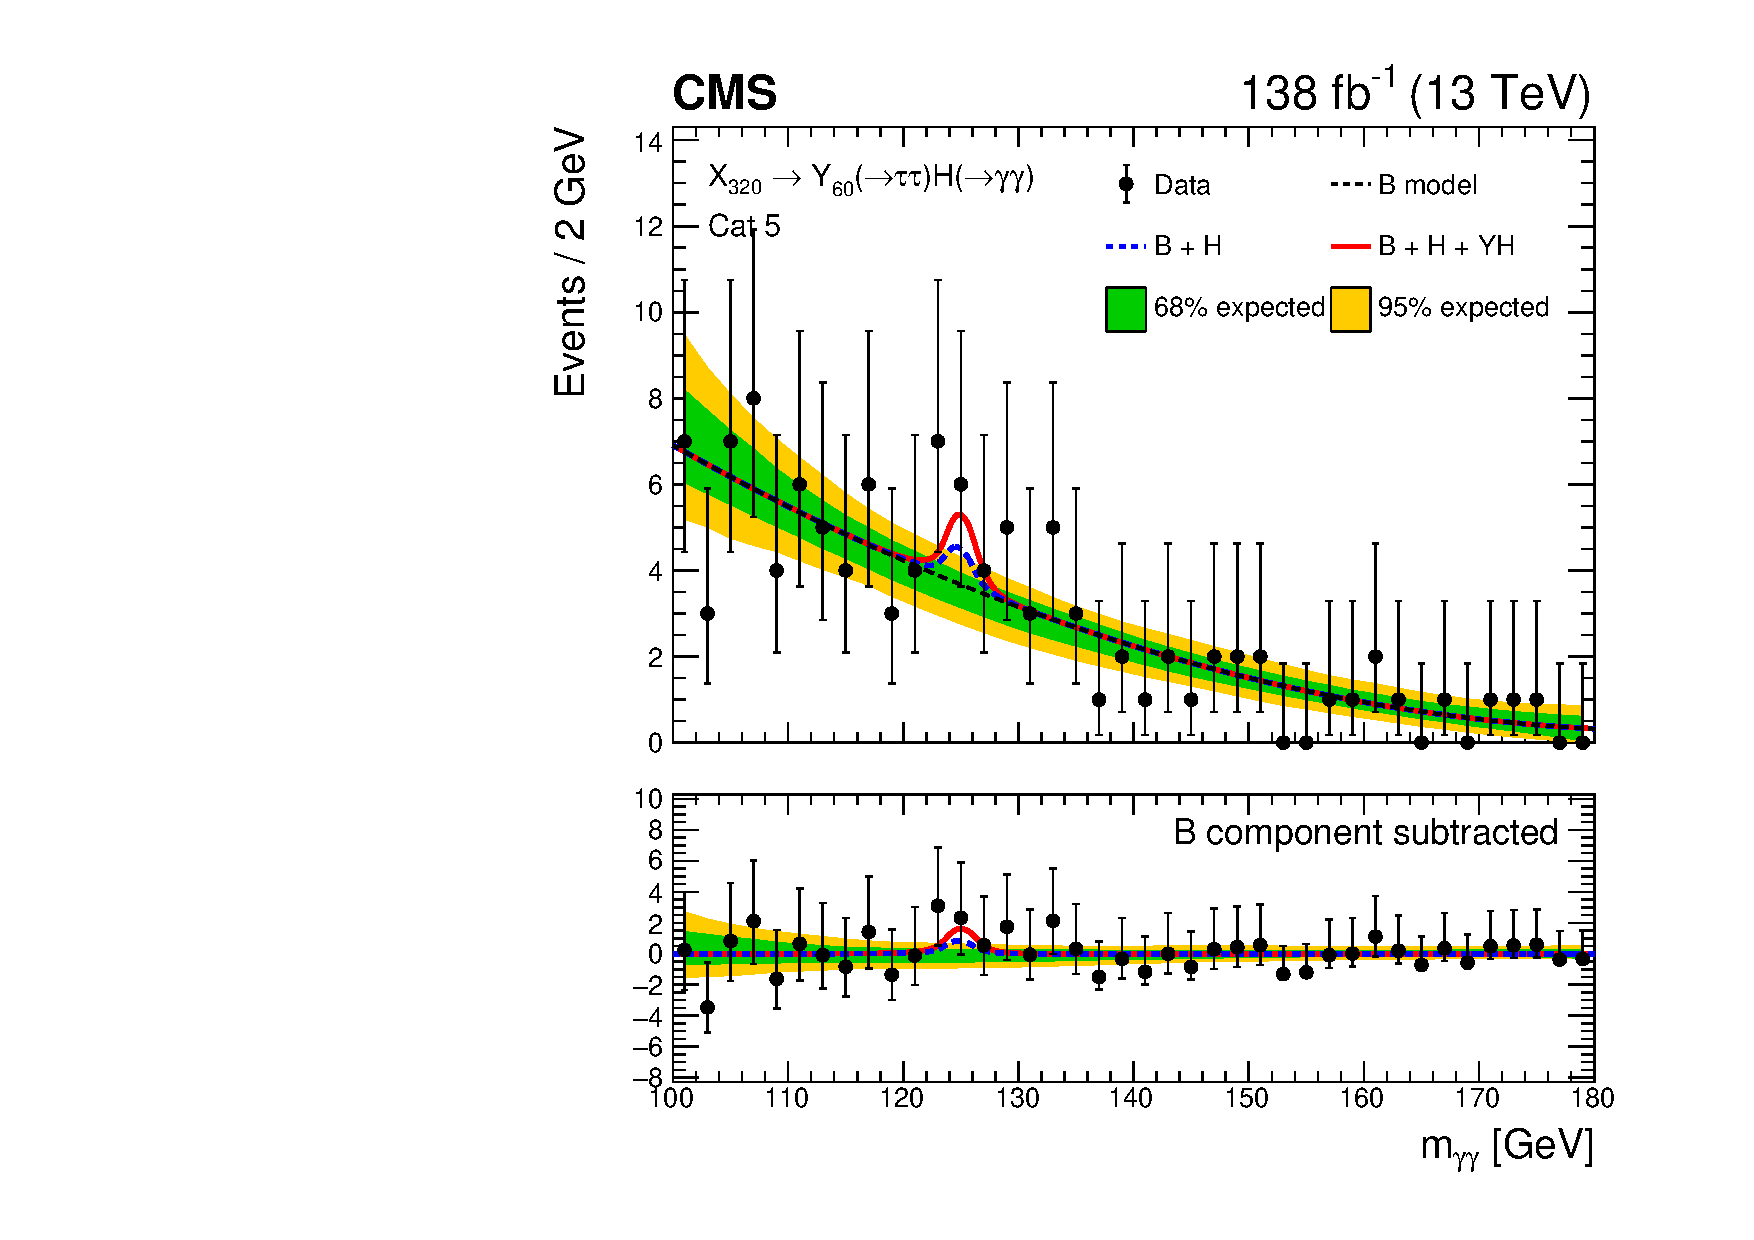
\includegraphics[width=.45\linewidth]{Figures/Dihiggs/results/sb_models/y_tautau/ARCGL_Y_tautau_mx320my60_ggttresmx320my60cat5_CMS_hgg_mass_nbins40_paper.pdf}
    \caption[Signal-Plus-Background Fits to Data for \XYttHgg Search at $(\mX,\mY)=(320,60)$\GeV]{Distributions of \mgg in data in each analysis category and the signal-plus-background models (red) with data (black points) for the mass hypothesis with the largest excess in the \XYttHgg search: $(\mX,\mY)=(320,60)$\GeV. The one (green) standard deviation and two (yellow) standard deviation bands show the uncertainties in the nonresonant background component of the model (black dashed line). The resonant single-Higgs background is plotted separately in blue (blue dashed line). The lower panel shows the residuals after subtraction of the nonresonant background component.}\label{fig:sbmodel_2}
\end{figure}

The observed 95\% CL upper limits on $\sigma(\ppXYHggtt)$ for the \XYttHgg search are shown in a 2D heatmap in \cref{fig:limits_2d_obs_y_tautau}, and the expected and observed limits are shown in slices of \mX and \mY in \cref{fig:limits_stack_mx_y_tautau,fig:limits_stack_my_y_tautau}, respectively, where the slices are taken at the nominal mass points. Like in the \XHH searches, the lowest limits are set at higher values of \mX, and the highest limits are found at lower \mX, particularly in the band where the highest significances are found. There is less of a noticeable trend in \mY, which is reflected in the preselection signal efficiency (\cref{fig:presel_eff_xyh}). The observed (expected) upper limits vary between 0.059--1.2\fb (0.087--0.68\fb), depending on the mass point. 

\begin{figure}
    \centering
    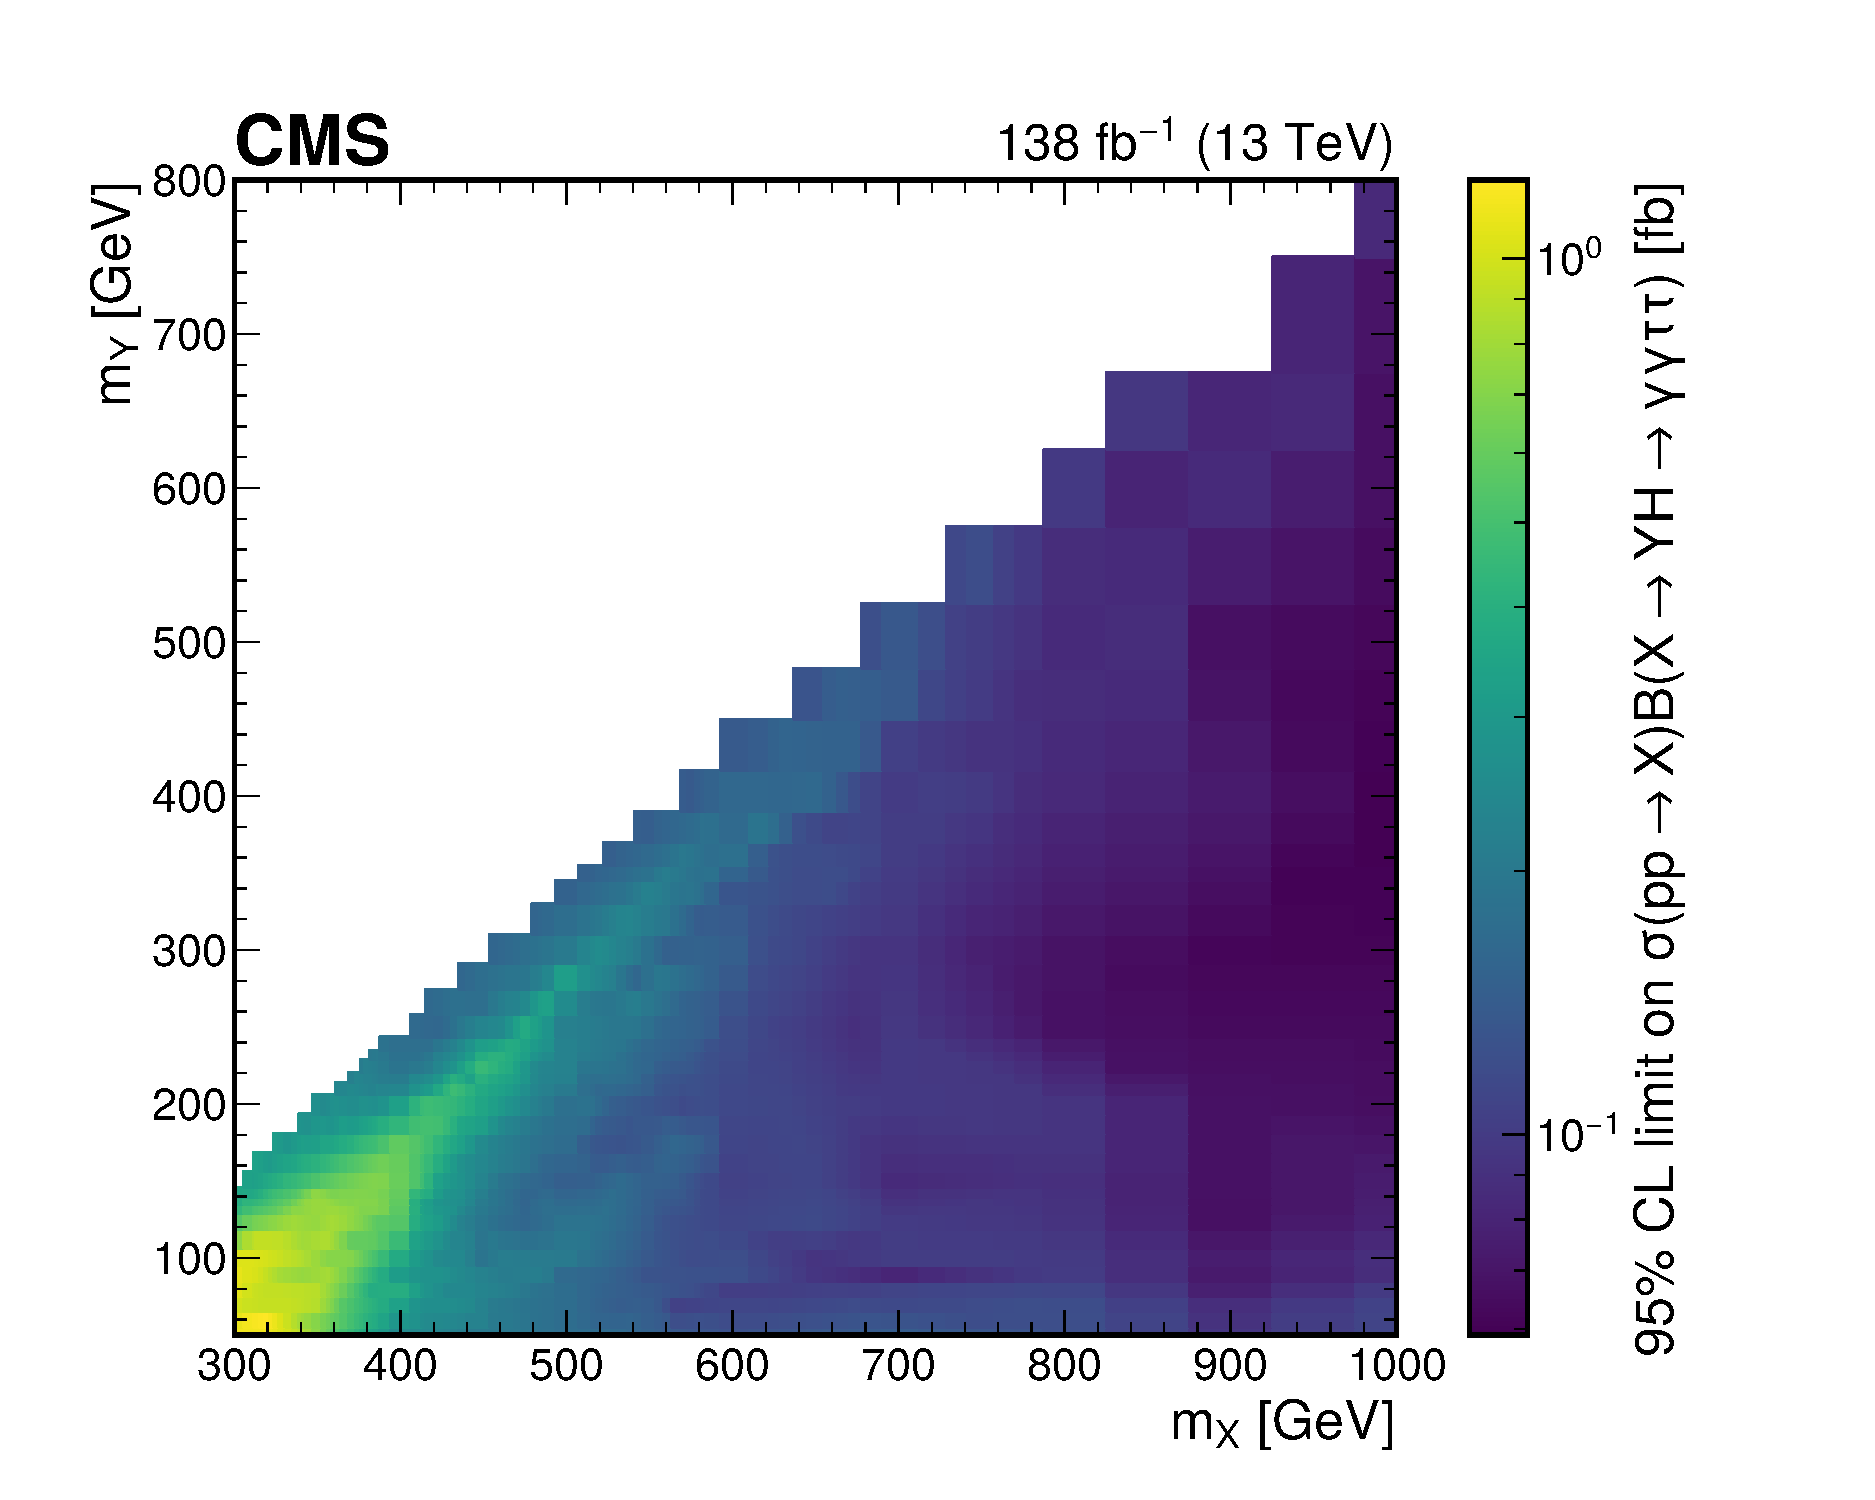
\includegraphics[width=0.8\textwidth]{Figures/Dihiggs/results/limits/limits_2d_obs_y_tautau_paper.pdf}
    \caption[\XYttHgg Upper Limits in the 2D $(\mX,\mY)$ Plane]{Observed 95\% CL upper limits on $\sigma(\ppXYHggtt)$ in the 2D $(\mX,\mY)$ plane for the \XYttHgg search.}\label{fig:limits_2d_obs_y_tautau}
\end{figure}

\begin{figure}
    \centering
    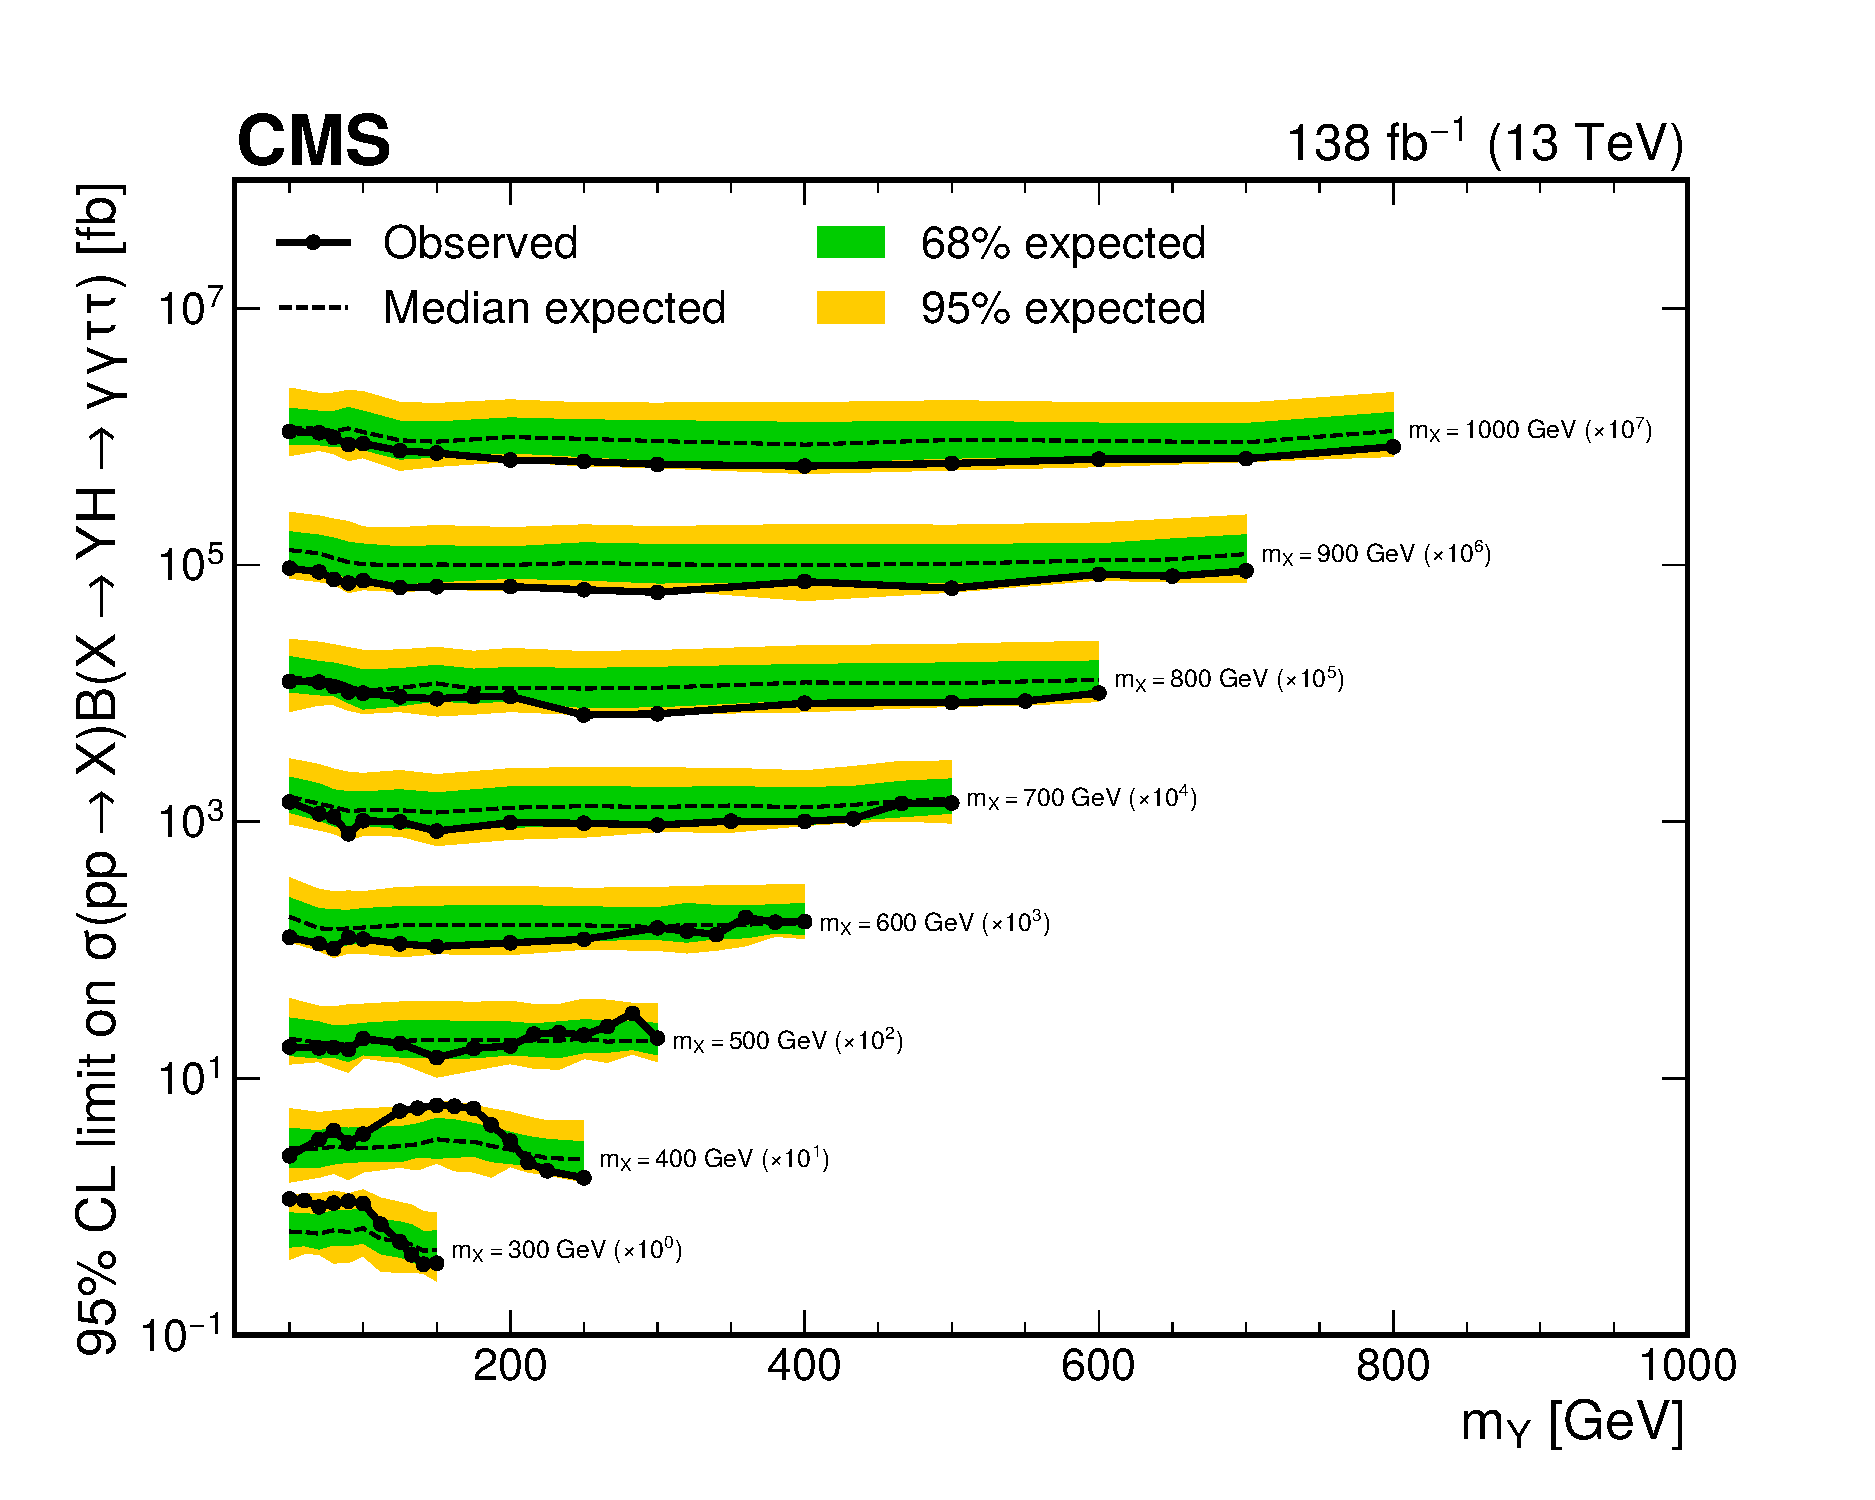
\includegraphics[width=\textwidth]{Figures/Dihiggs/results/limits/limits_stack_mx_y_tautau_paper.pdf}
    \caption[\XYttHgg Upper Limits in as Function of \mY in Slices of \mX]{Expected and observed 95\% CL upper limits on $\sigma(\ppXYHggtt)$ for the \XYttHgg search. Limits are shown as a function of \mY for the nominal values of \mX where the limits are scaled by orders of 10 as labelled in the plot. The solid and dashed black lines represent observed and median expected limits respectively. The inner (green) band and the outer (yellow) band indicate the regions containing 68 and 95\%, respectively, of the distribution of limits expected under the background-only hypothesis.}\label{fig:limits_stack_mx_y_tautau}
\end{figure}
\begin{figure}
    \centering
    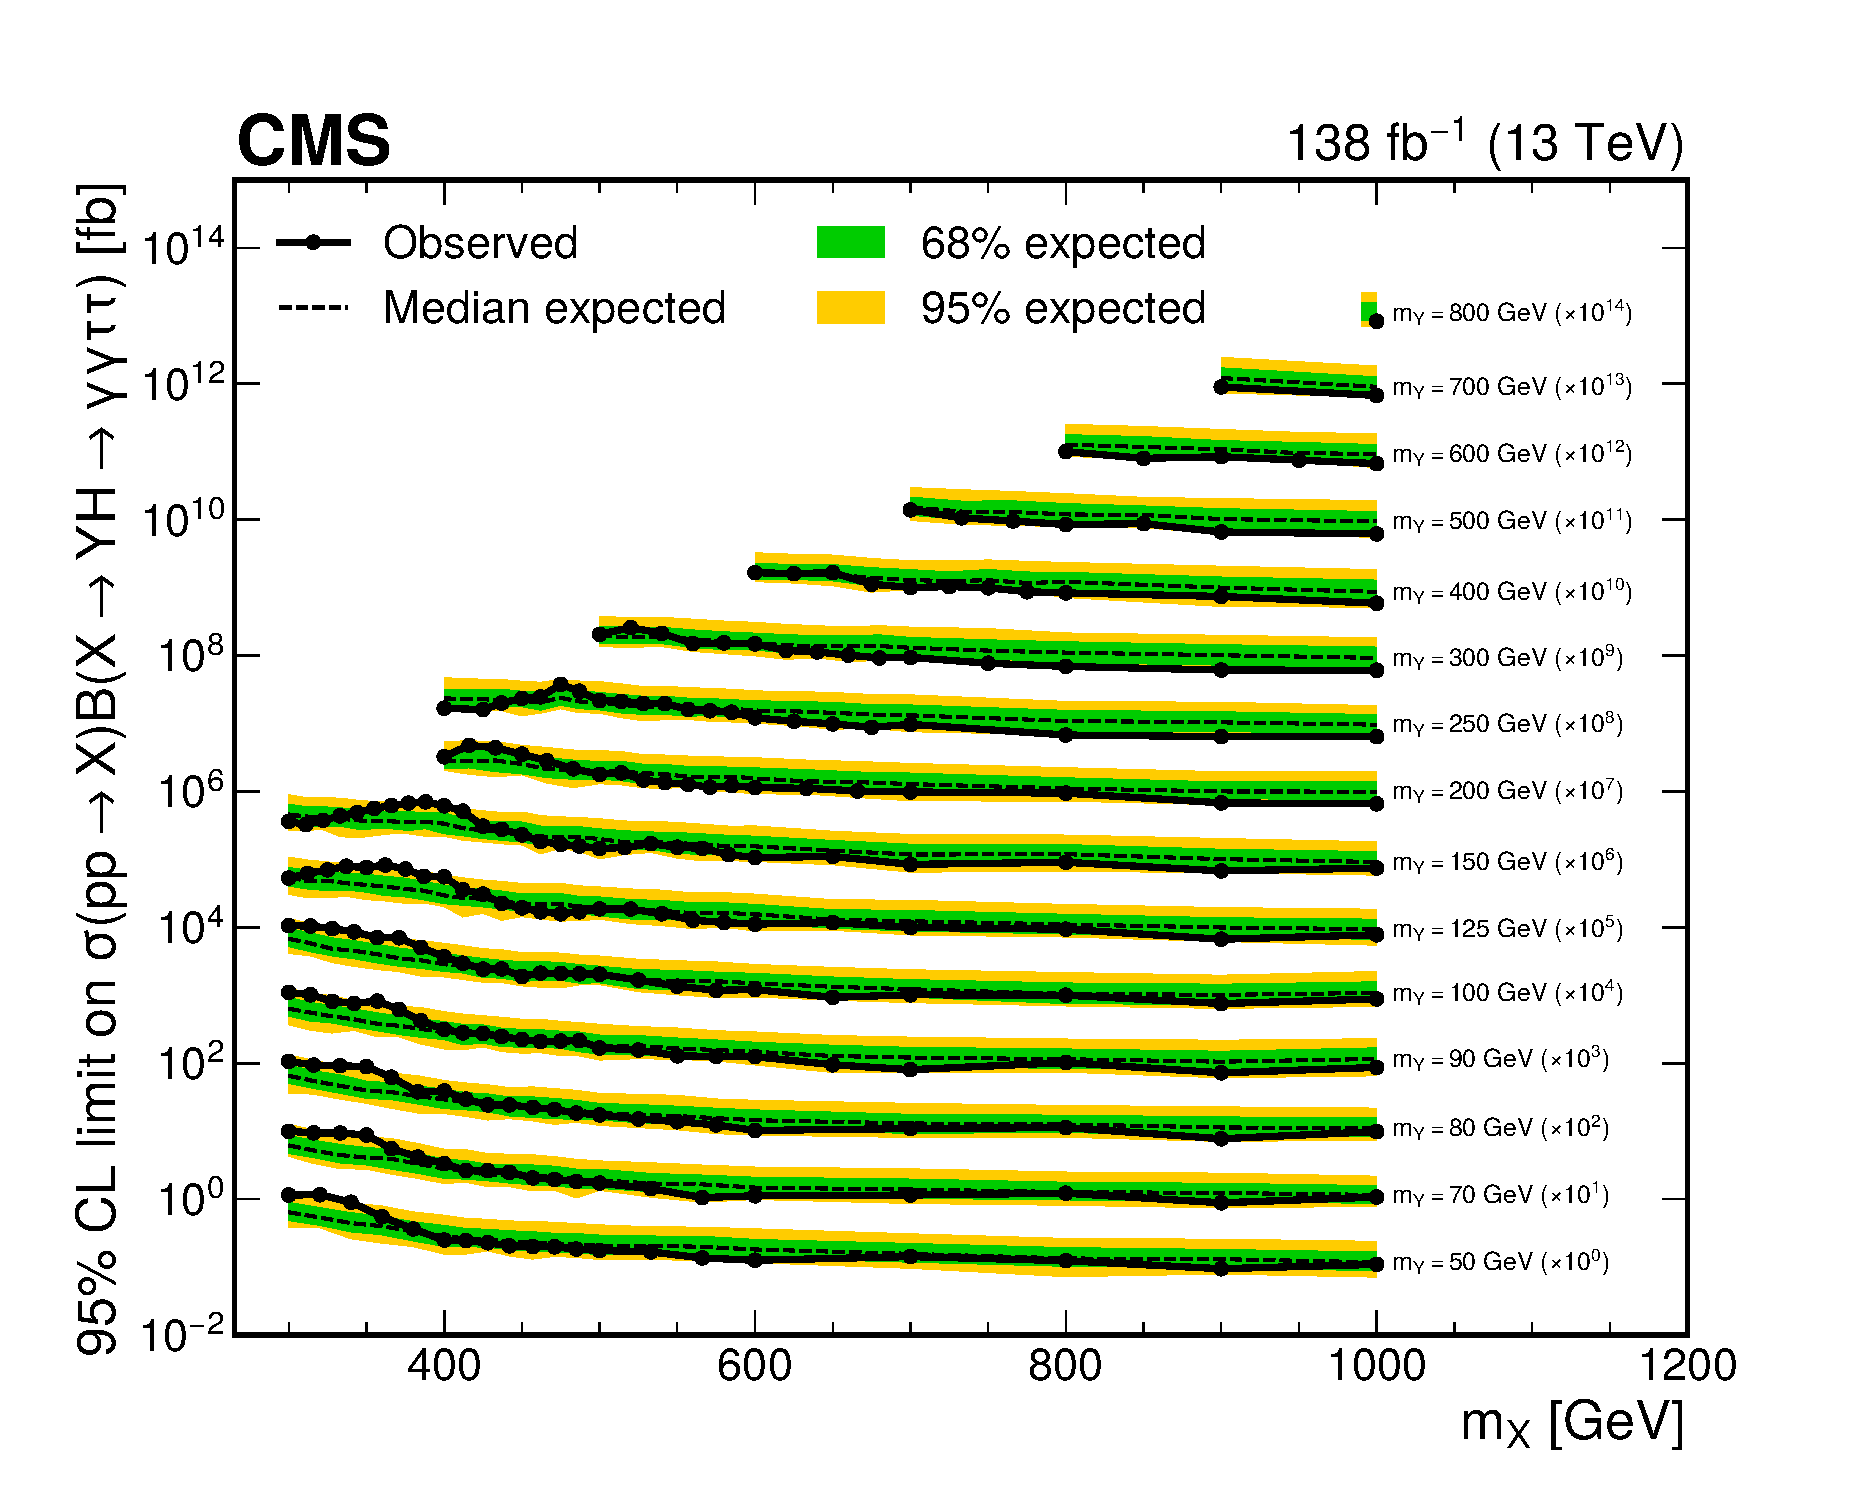
\includegraphics[width=\textwidth]{Figures/Dihiggs/results/limits/limits_stack_my_y_tautau_paper.pdf}
    \caption[\XYttHgg Upper Limits in as Function of \mX in Slices of \mY]{Expected and observed 95\% CL upper limits on $\sigma(\ppXYHggtt)$ for the \XYttHgg search. Limits are shown as a function of \mX for the nominal values of \mY where the limits are scaled by orders of 10 as labelled in the plot. The solid and dashed black lines represent observed and median expected limits respectively. The inner (green) band and the outer (yellow) band indicate the regions containing 68 and 95\%, respectively, of the distribution of limits expected under the background-only hypothesis.}\label{fig:limits_stack_my_y_tautau}
\end{figure}

In the \bbgg final state~\cite{CMS:2023boe}, observed upper limits on the equivalent cross section: $\sigma(\ppXYHbbgg)$, were found to be about 0.04--0.90\fb. Therefore, for models where $\BR(\Ytt)$ and $\BR(\Ybb)$ are similar, the \ggtt final state provides a similar sensitivity to the \bbgg final state. Furthermore, this search in the \ggtt state searched for \PY resonances with masses down to 50\GeV whereas the \bbgg search only went down to 70\GeV. 

\subsection[Low-Mass \texorpdfstring{\XYggHtt}{XY(tt)H(gg)} Search]{Low-Mass \XYggHtt Search}\label{sec:results_y_gg_low_mass}

\Cref{fig:significance_y_gg_low_mass} shows the local significances for every mass point in the low-mass \XYggHtt search. Compared to the \XYttHgg search, there is less structure in the significance plot, owing to the fact that changing $\mY$ now changes the location of the \mgg peak in the signal model, as well as the pNN selection as before. The largest excess is seen at $(\mX,\mY)=(525,115)$\GeV, with a local significance of 3.2 standard deviations. The \mgg distributions in data for this mass point, and the corresponding signal-plus-background model fit, is shown in \cref{fig:sbmodel_3}. The excess is driven primarily by a low background prediction and 2 events near $\mgg=115$\GeV in category 0. 



There is also an excess with a significance of 2.3 standard deviations at $(\mX, \mY) = (650, 95)$\GeV, which is particularly interesting due to recent excesses seen by the CMS experiment at similar mass points (see \cref{sec:ggtt_intro}). Importantly, from \cref{fig:significance_y_gg_low_mass}, the excess also appears to be fairly localized to $(\mX, \mY) = (650, 95)$\GeV, which gives the coincidence of the excesses in different final states more weight. The \mgg distributions in data for this mass point, and the corresponding signal-plus-background model fit, is shown in \cref{fig:sbmodel_6}. The excess is similarly driven by a low background prediction and 2 events near $\mgg=95$\GeV in category 0.



At this mass point, \mY is closer to \mZ and therefore, the DY background modelling may be more important. However, the expected number of DY events is at most 0.27 events across all categories, and noticeably smaller than the extracted signal peak in category 0 seen in \cref{fig:sbmodel_6} (top-right). Given that the normalization of the DY background is small, and that it's peak does not have significant overlap with the signal peak, the impact on the significance is small, where removing the DY background model entirely changes the significance by less than 0.1 standard deviations. At other mass points, where there is greater overlap between the DY background and the signal, the impact on the results is still small. For the $(\mX, \mY) = (1000, 90)$\GeV mass point, which has one of the largest expected number of DY events (\cref{sec:dy_bkg_modelling}), the observed and expected upper limits change by 2\% when removing the DY background modelling.

The global significance of the low-mass \XYggHtt search is only 0.1 standard deviations. Compared to the \XYttHgg search, the look-elsewhere effect is larger due to the greater (about a factor of five) number of mass points searched at. Therefore, as a standalone result, the excesses at $(\mX,\mY)=(525,115)$\GeV and $(650,95)$\GeV are not particularly interesting. However, the excess at $(\mX,\mY)=(650,95)$\GeV is interesting given the recent excesses seen with 650 and $\sim95$\GeV resonances (\cref{sec:ggtt_intro}).  

The observed 95\% CL upper limits on $\sigma(\ppXYH)\BR(\Ygg)$ for the low-mass \XYggHtt search are shown in a 2D heatmap in \cref{fig:limits_2d_obs_y_gg_low_mass}, and the expected and observed limits are shown in slices of \mX and \mY in \cref{fig:limits_stack_mx_y_gg_low_mass,fig:limits_stack_my_y_gg_low_mass}, respectively, where the slices are taken at the nominal mass points. Similar trends in \mX and \mY are seen in the limits as in the \XYttHgg search, and the observed (expected) upper limits vary between 0.69--15\fb (0.73--8.3\fb), depending on the mass point. 

The observed limits are compared to the maximally-allowed values in the NMSSM given experimental constraints (\cref{sec:low_mass_in_NMSSM}), and the region of masses where the limit is below the maximally-allowed value is shown in \cref{fig:limits_2d_obs_y_gg_low_mass}. For most values of \mY in the low-mass \XYggHtt search, this region corresponds to $\mX < 650$\GeV, or for all values of \mY in the search, this region corresponds to $\mX < 620$\GeV. This implies that these results can be used to apply tighter constraints on the NMSSM parameter space than previously possible. Deriving those constraints is beyond the scope of this thesis, but could be done in a future iteration of the work presented in Ref.~\cite{Ellwanger:2022jtd}.

\begin{figure}
    \centering
    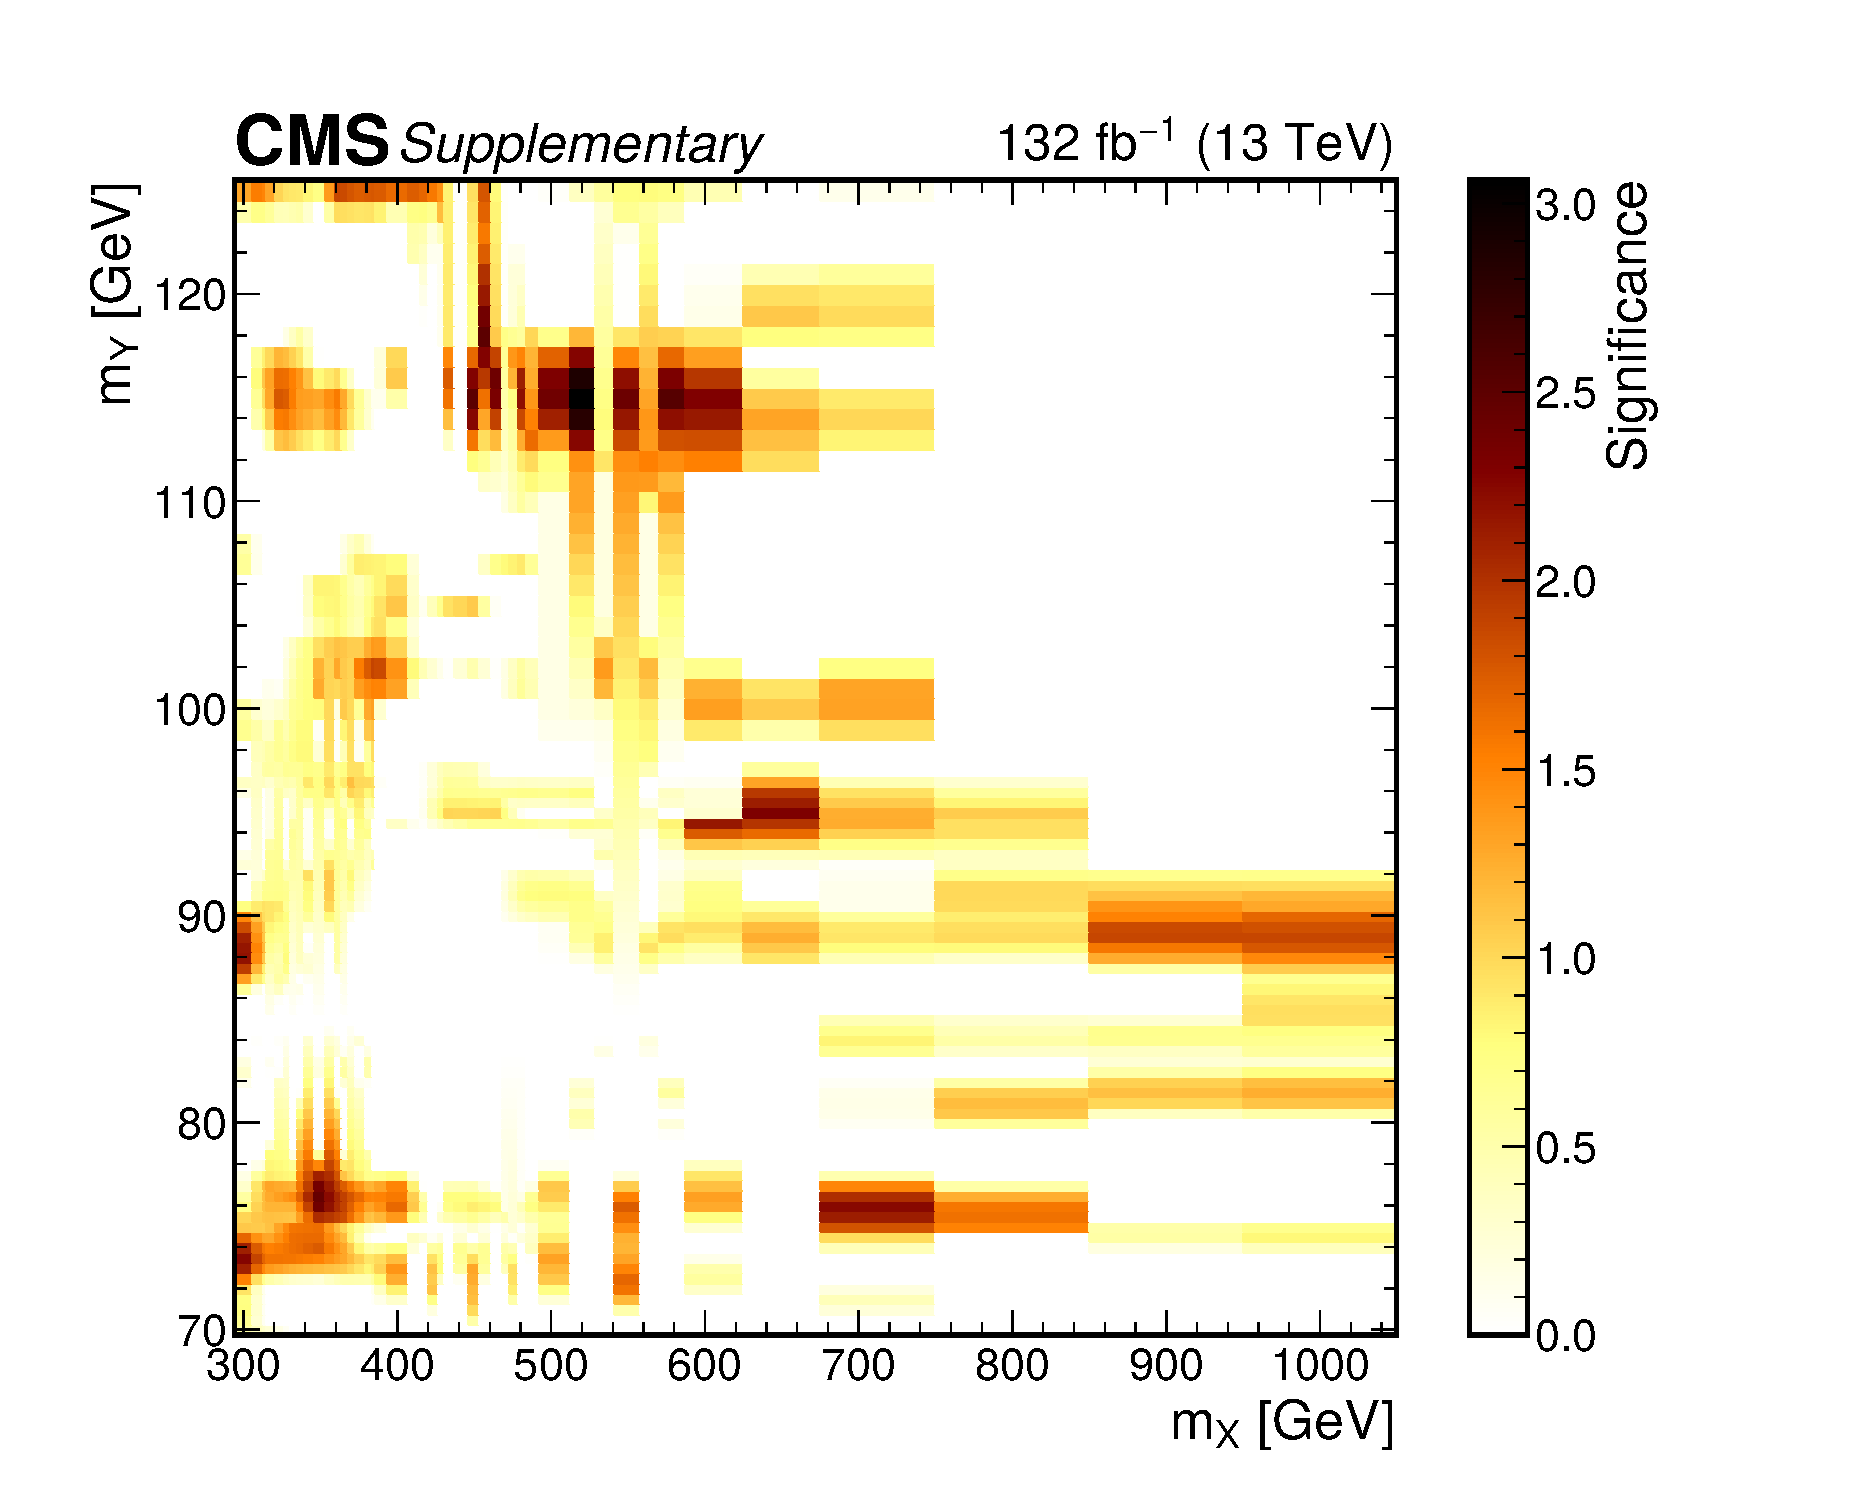
\includegraphics[width=0.8\textwidth]{Figures/Dihiggs/results/significances/significance_y_gg_low_mass_supplementary.pdf}
    \caption[Low-Mass \XYggHtt Observed Local Significances]{Observed local significances in the 2D $(\mX,\mY)$ plane for the low-mass \XYggHtt search.}\label{fig:significance_y_gg_low_mass}
\end{figure}

\begin{figure}
    \centering
    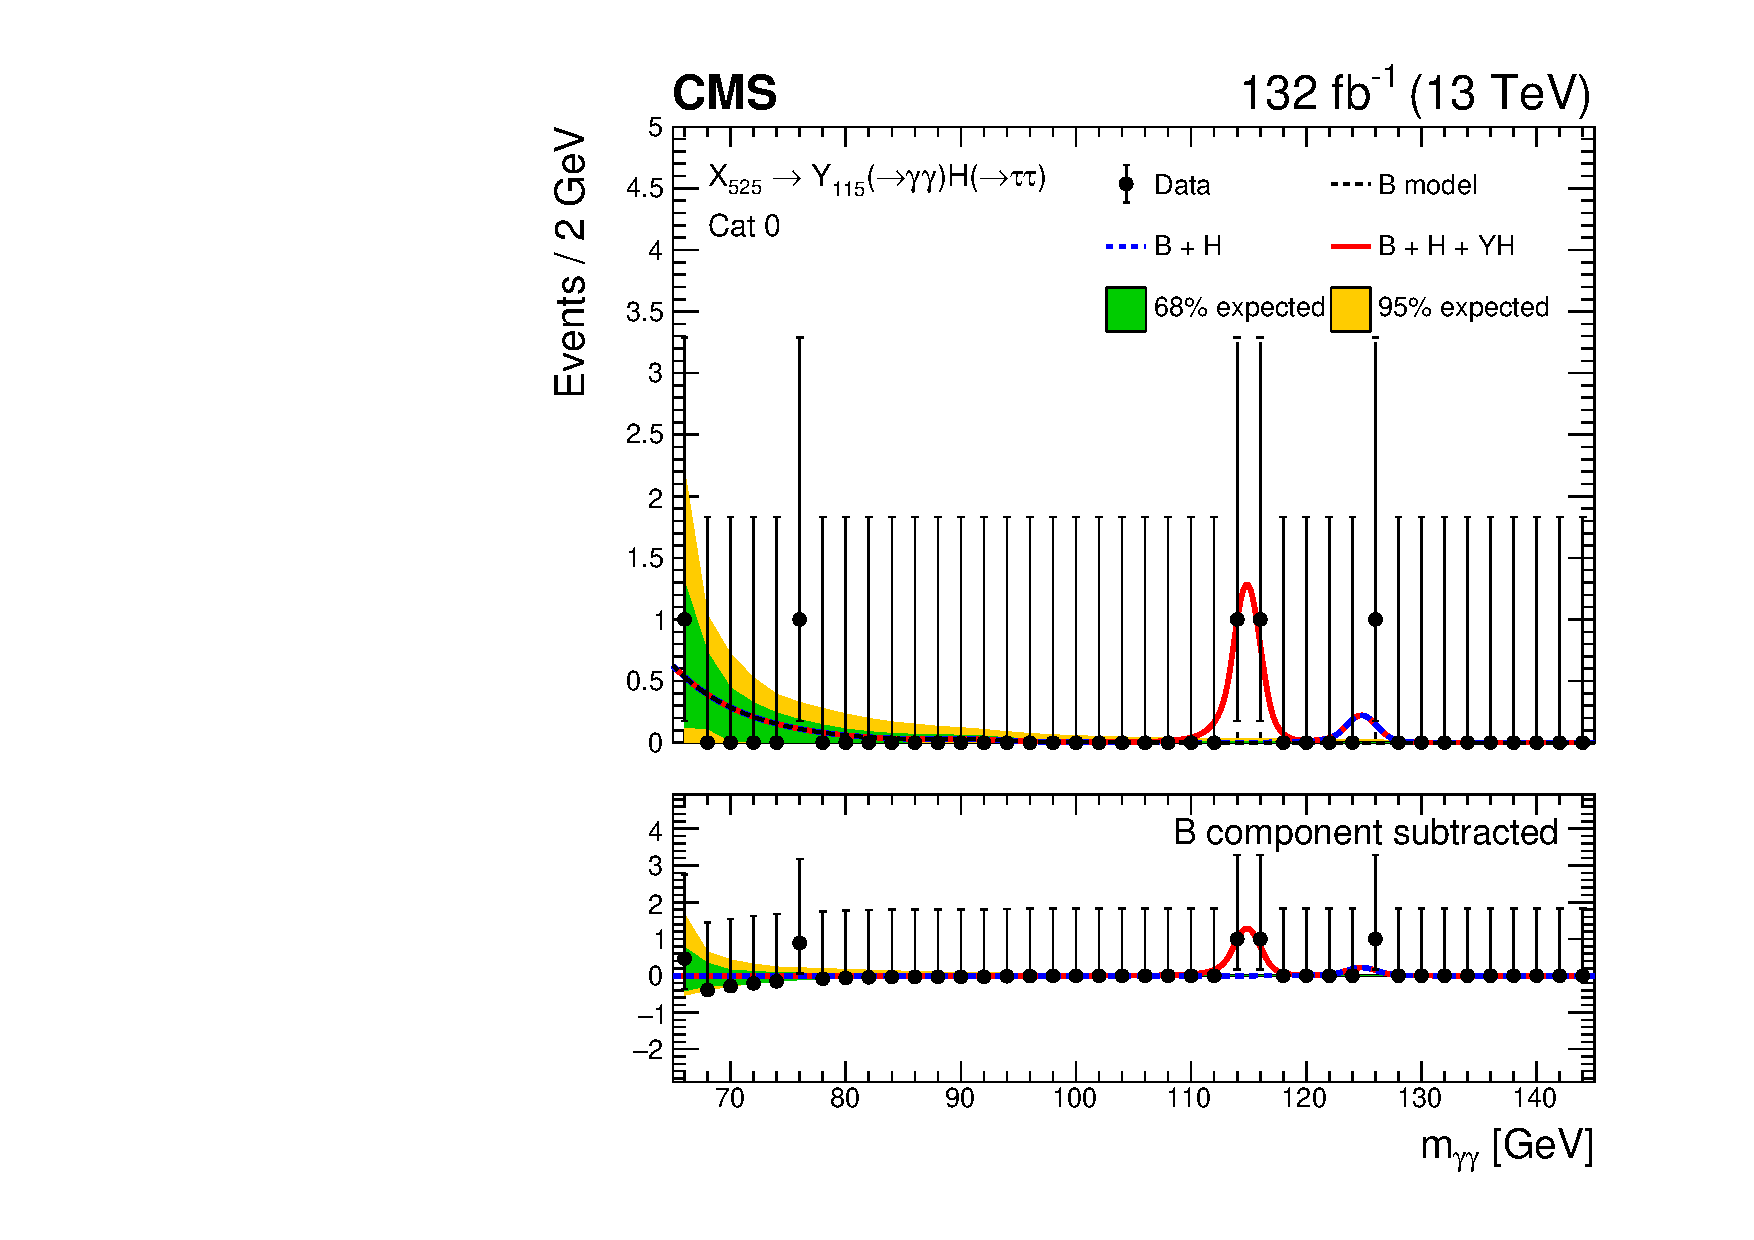
\includegraphics[width=.45\linewidth]{Figures/Dihiggs/results/sb_models/y_gg_low_mass/ARCGL_Y_gg_Low_Mass_mx525my125mh115_ggttresmx525my125cat0_CMS_hgg_mass_nbins40_paper.pdf}
    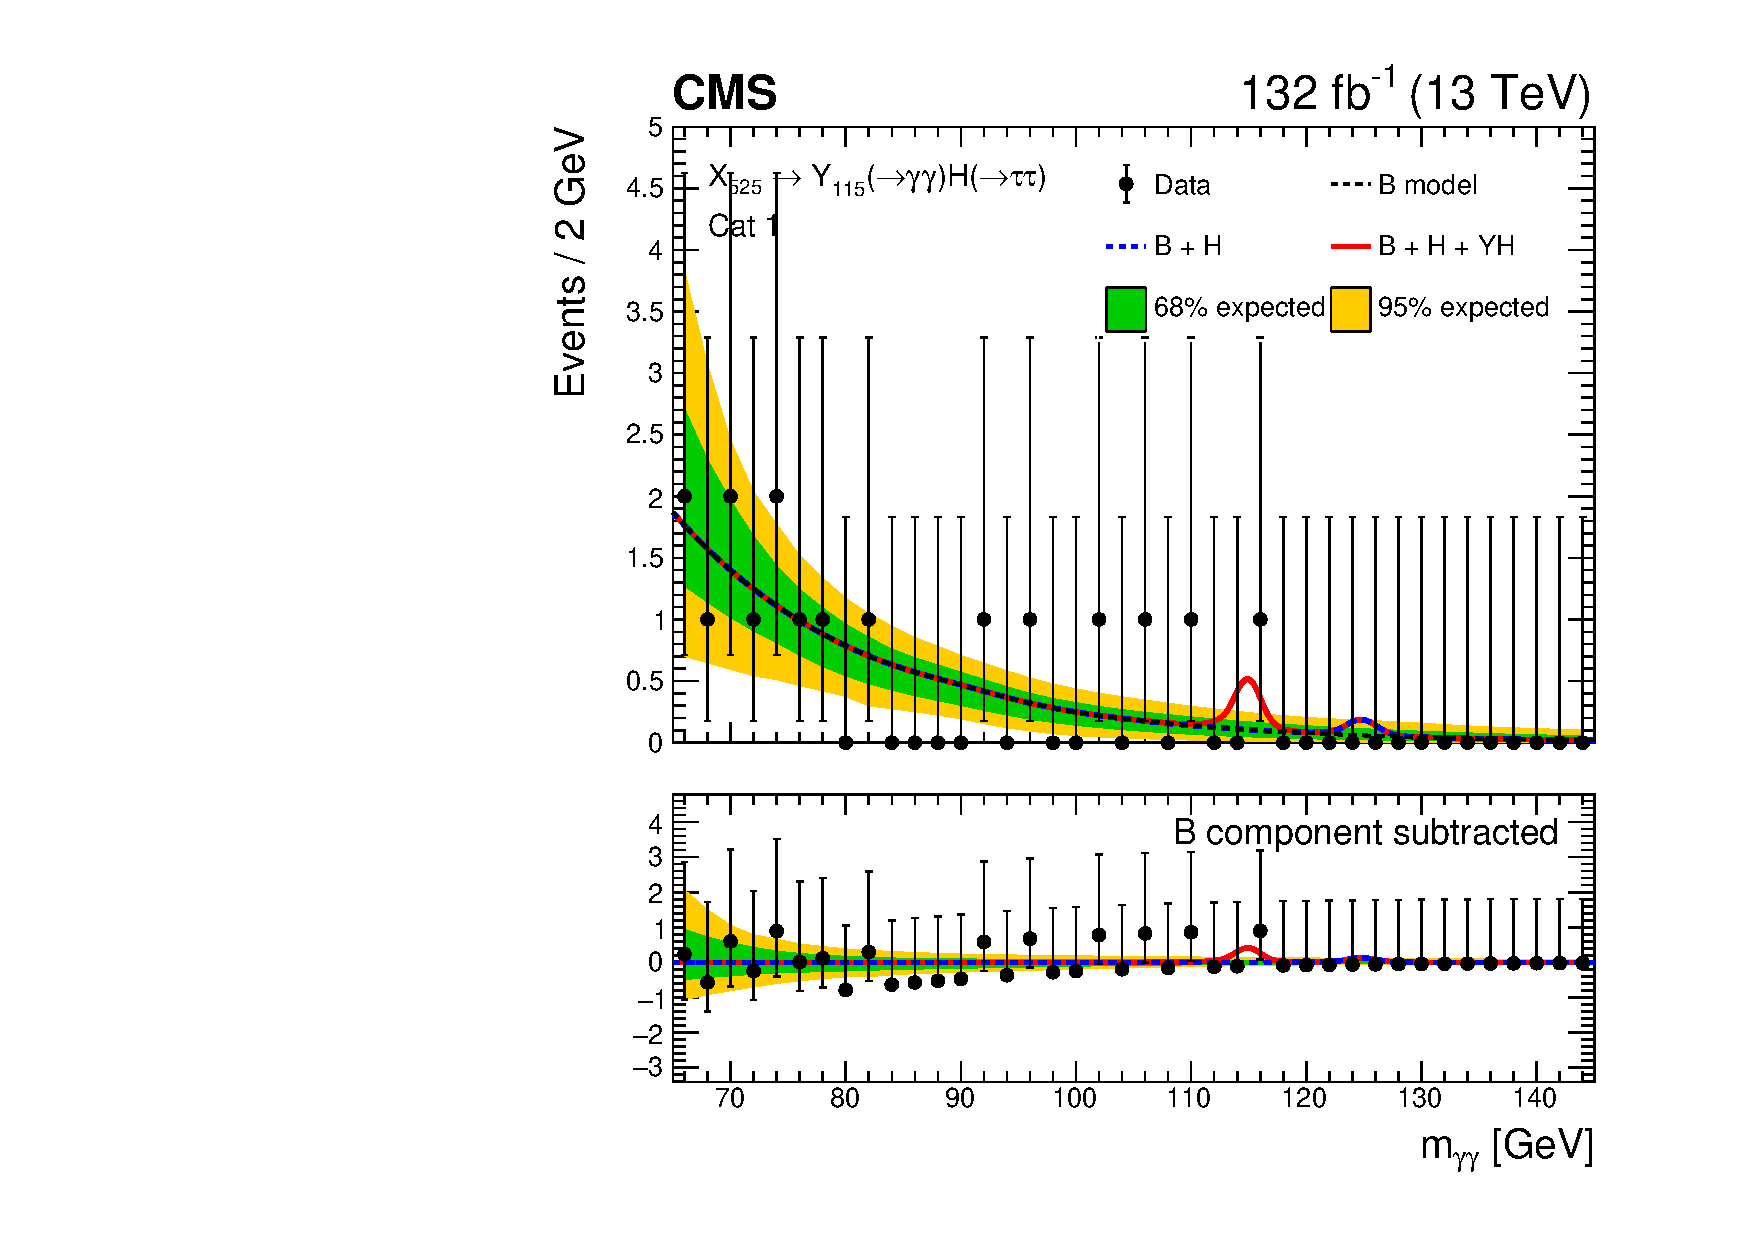
\includegraphics[width=.45\linewidth]{Figures/Dihiggs/results/sb_models/y_gg_low_mass/ARCGL_Y_gg_Low_Mass_mx525my125mh115_ggttresmx525my125cat1_CMS_hgg_mass_nbins40_paper.pdf}
    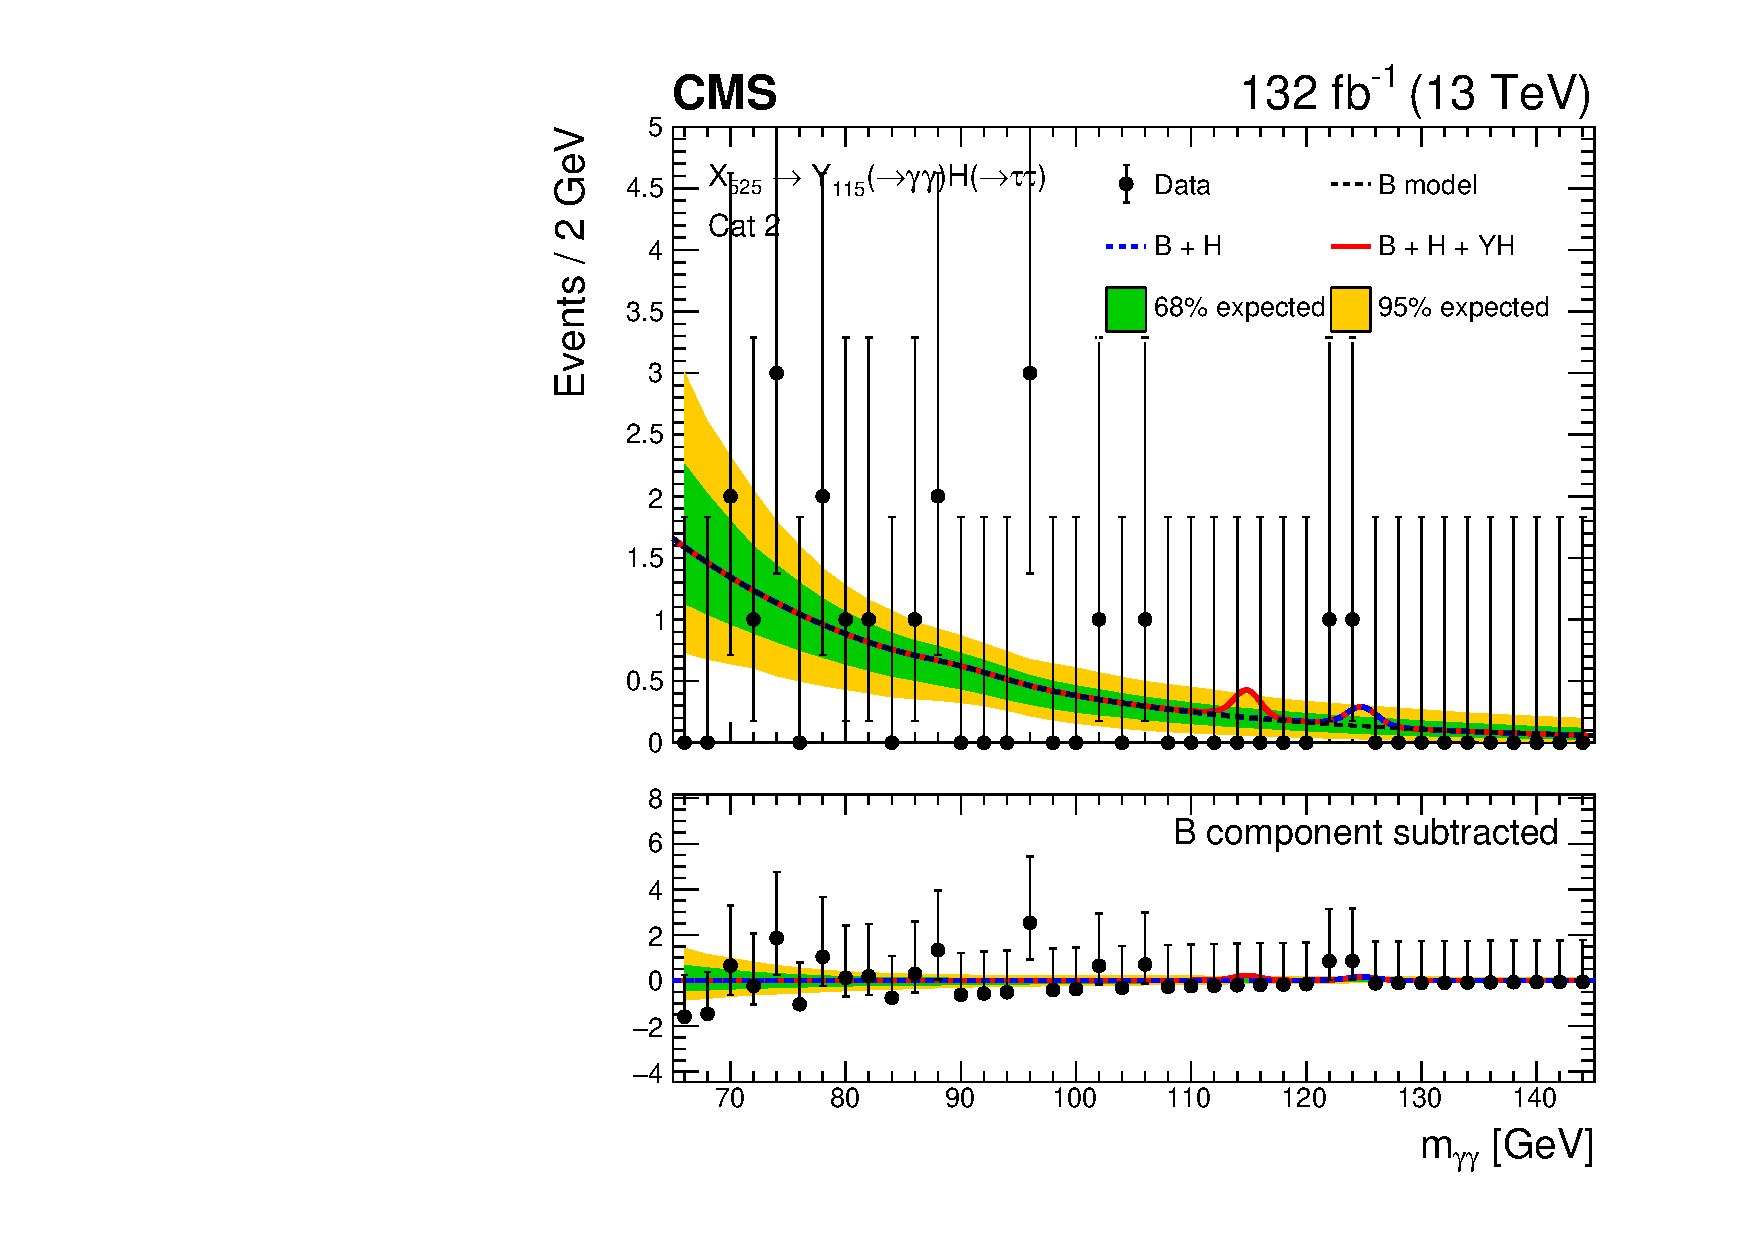
\includegraphics[width=.45\linewidth]{Figures/Dihiggs/results/sb_models/y_gg_low_mass/ARCGL_Y_gg_Low_Mass_mx525my125mh115_ggttresmx525my125cat2_CMS_hgg_mass_nbins40_paper.pdf}
    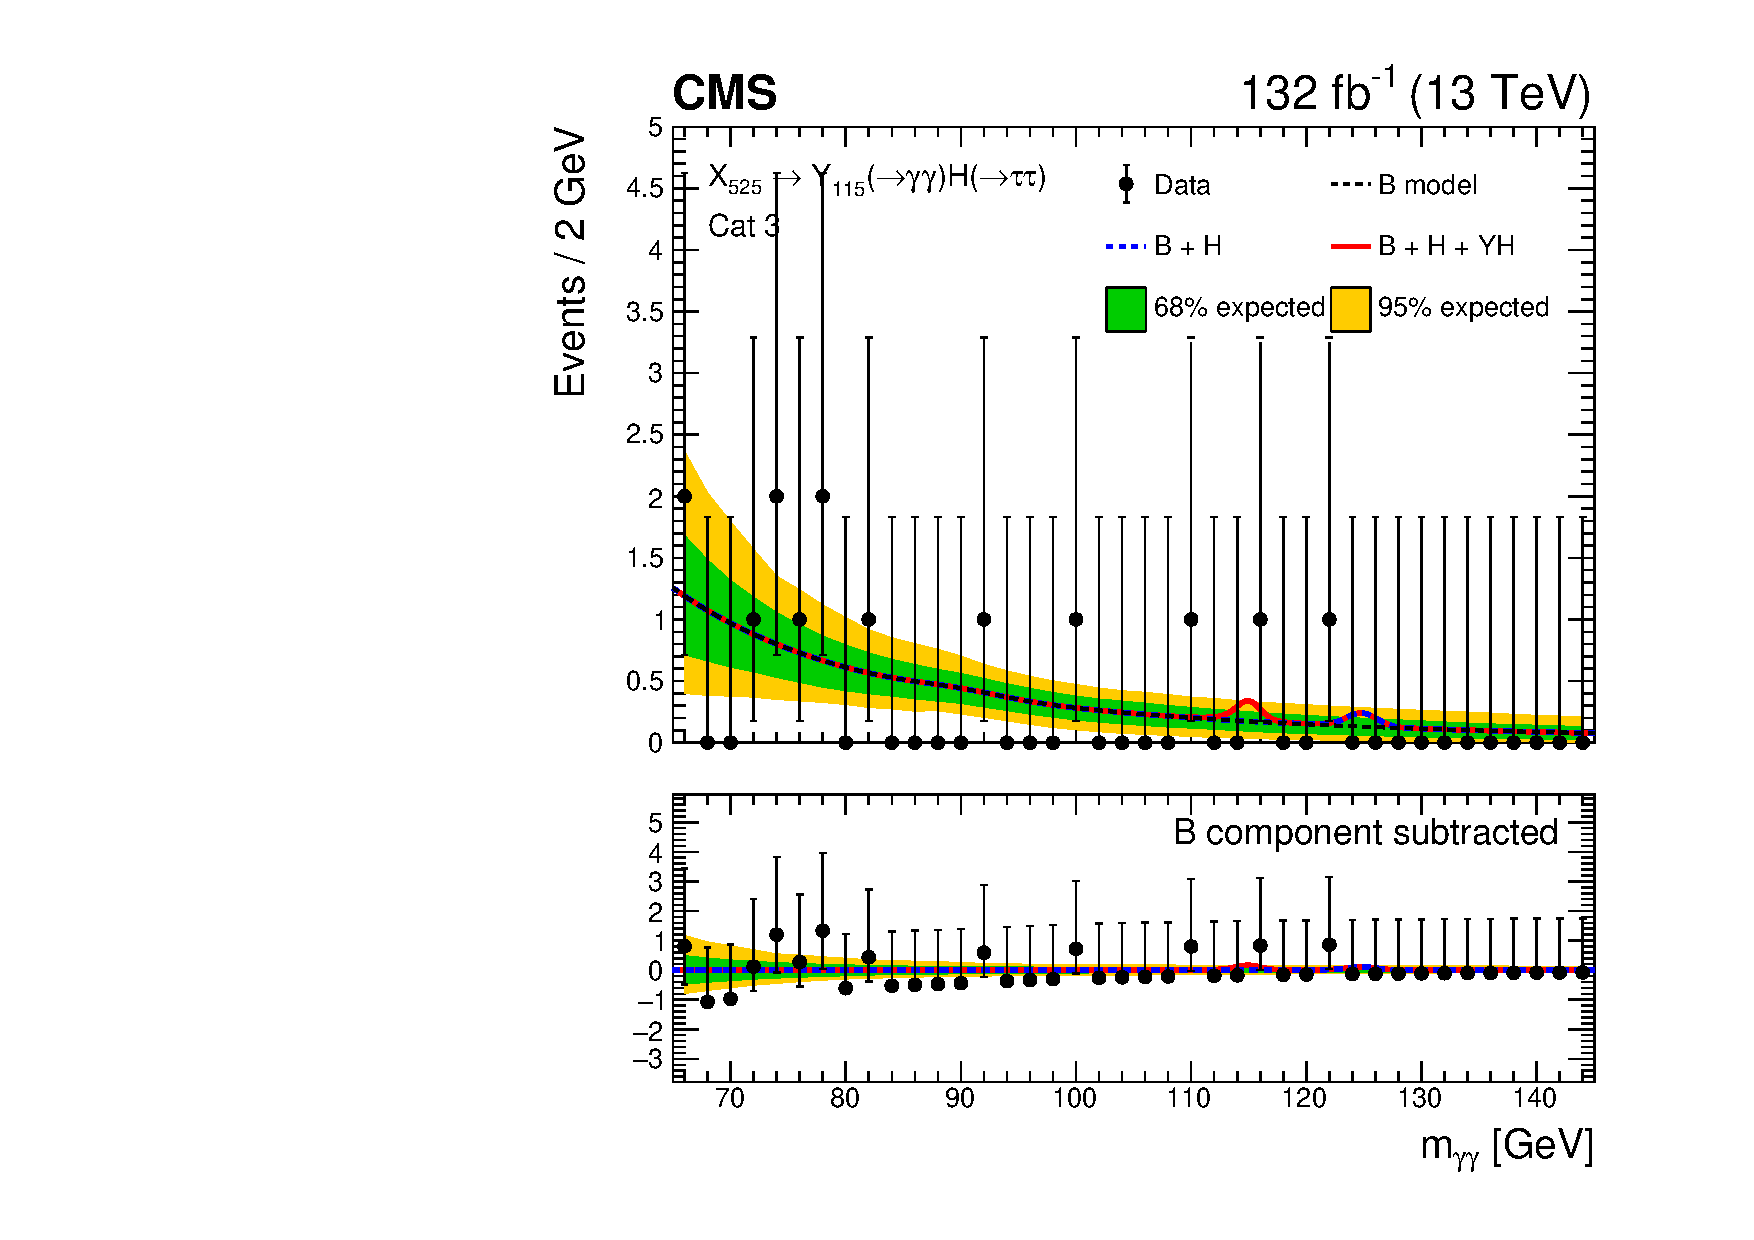
\includegraphics[width=.45\linewidth]{Figures/Dihiggs/results/sb_models/y_gg_low_mass/ARCGL_Y_gg_Low_Mass_mx525my125mh115_ggttresmx525my125cat3_CMS_hgg_mass_nbins40_paper.pdf}
    \caption[Signal-Plus-Background Fits to Data for Low-Mass \XYggHtt Search at $(\mX,\mY)=(525,115)$\GeV]{Distributions of \mgg in data in each analysis category corresponding to a signal region and the signal-plus-background models (red) with data (black points) for the mass hypothesis with the largest excess in the low-mass \XYggHtt search: $(\mX,\mY)=(525,115)$\GeV. The one (green) standard deviation and two (yellow) standard deviation bands show the uncertainties in the nonresonant + DY background component of the model (black dashed line). The resonant single-Higgs background is plotted separately in blue (blue dashed line). The lower panel shows the residuals after subtraction of the nonresonant background component.}\label{fig:sbmodel_3}
\end{figure}

\begin{figure}
    \centering
    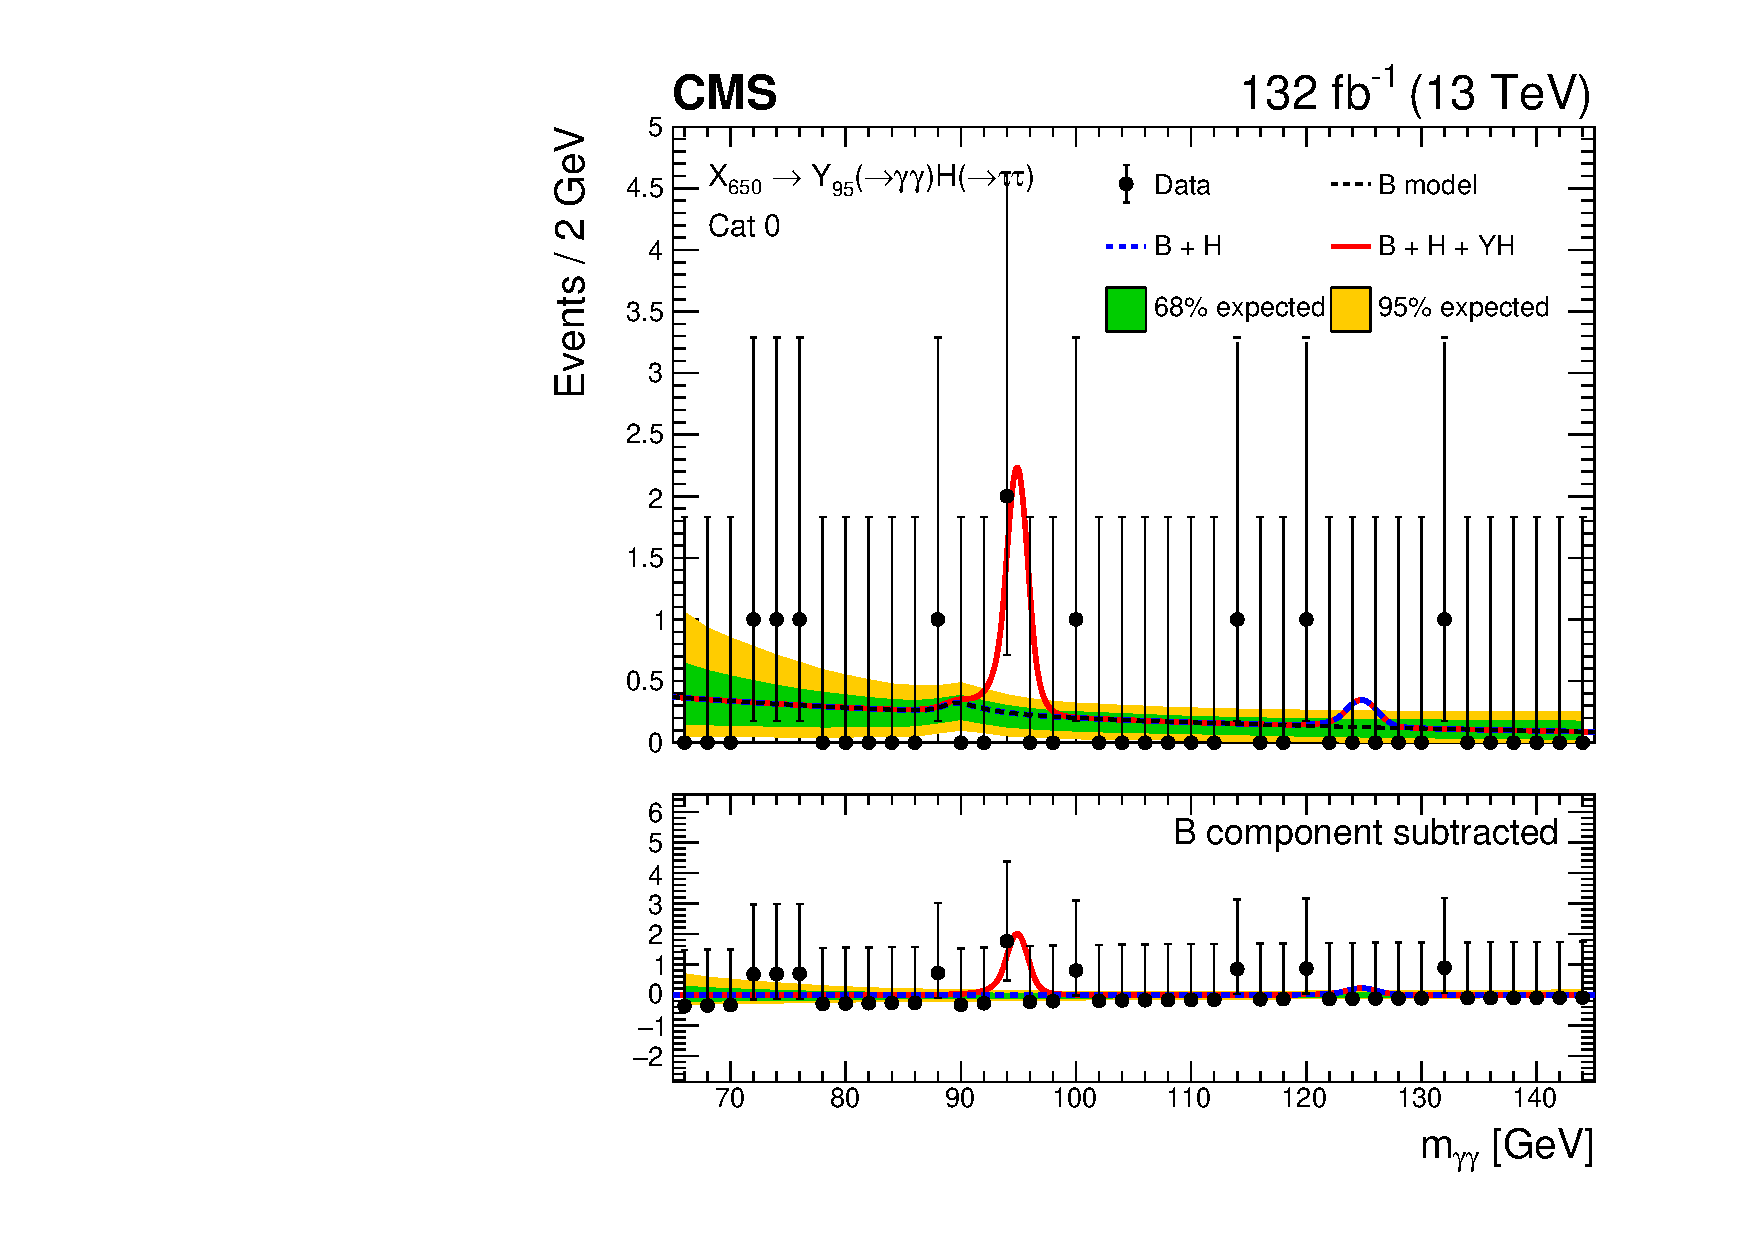
\includegraphics[width=.45\linewidth]{Figures/Dihiggs/results/sb_models/y_gg_low_mass_mx650my95/ARCGL_Y_gg_Low_Mass_mx650my100mh95_ggttresmx650my100cat0_CMS_hgg_mass_nbins40_paper.pdf}
    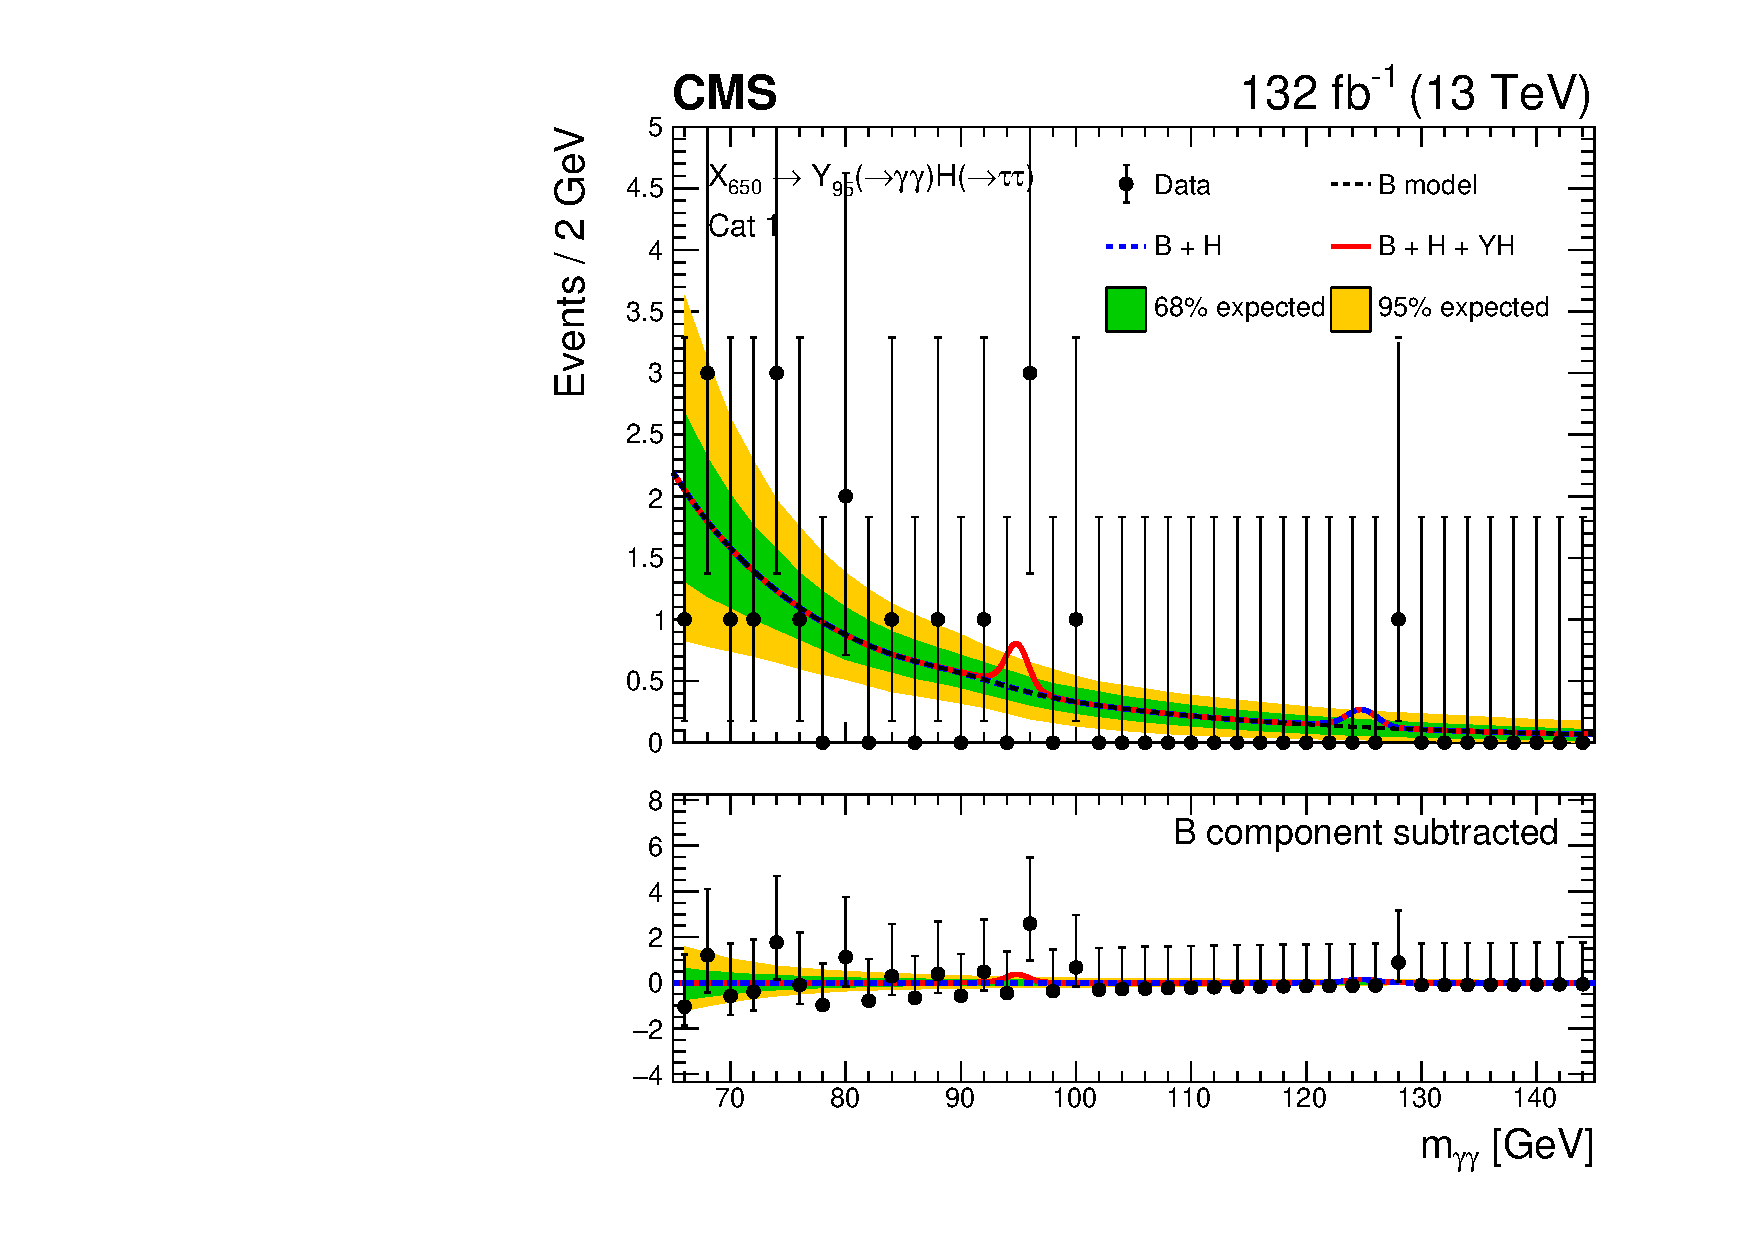
\includegraphics[width=.45\linewidth]{Figures/Dihiggs/results/sb_models/y_gg_low_mass_mx650my95/ARCGL_Y_gg_Low_Mass_mx650my100mh95_ggttresmx650my100cat1_CMS_hgg_mass_nbins40_paper.pdf}
    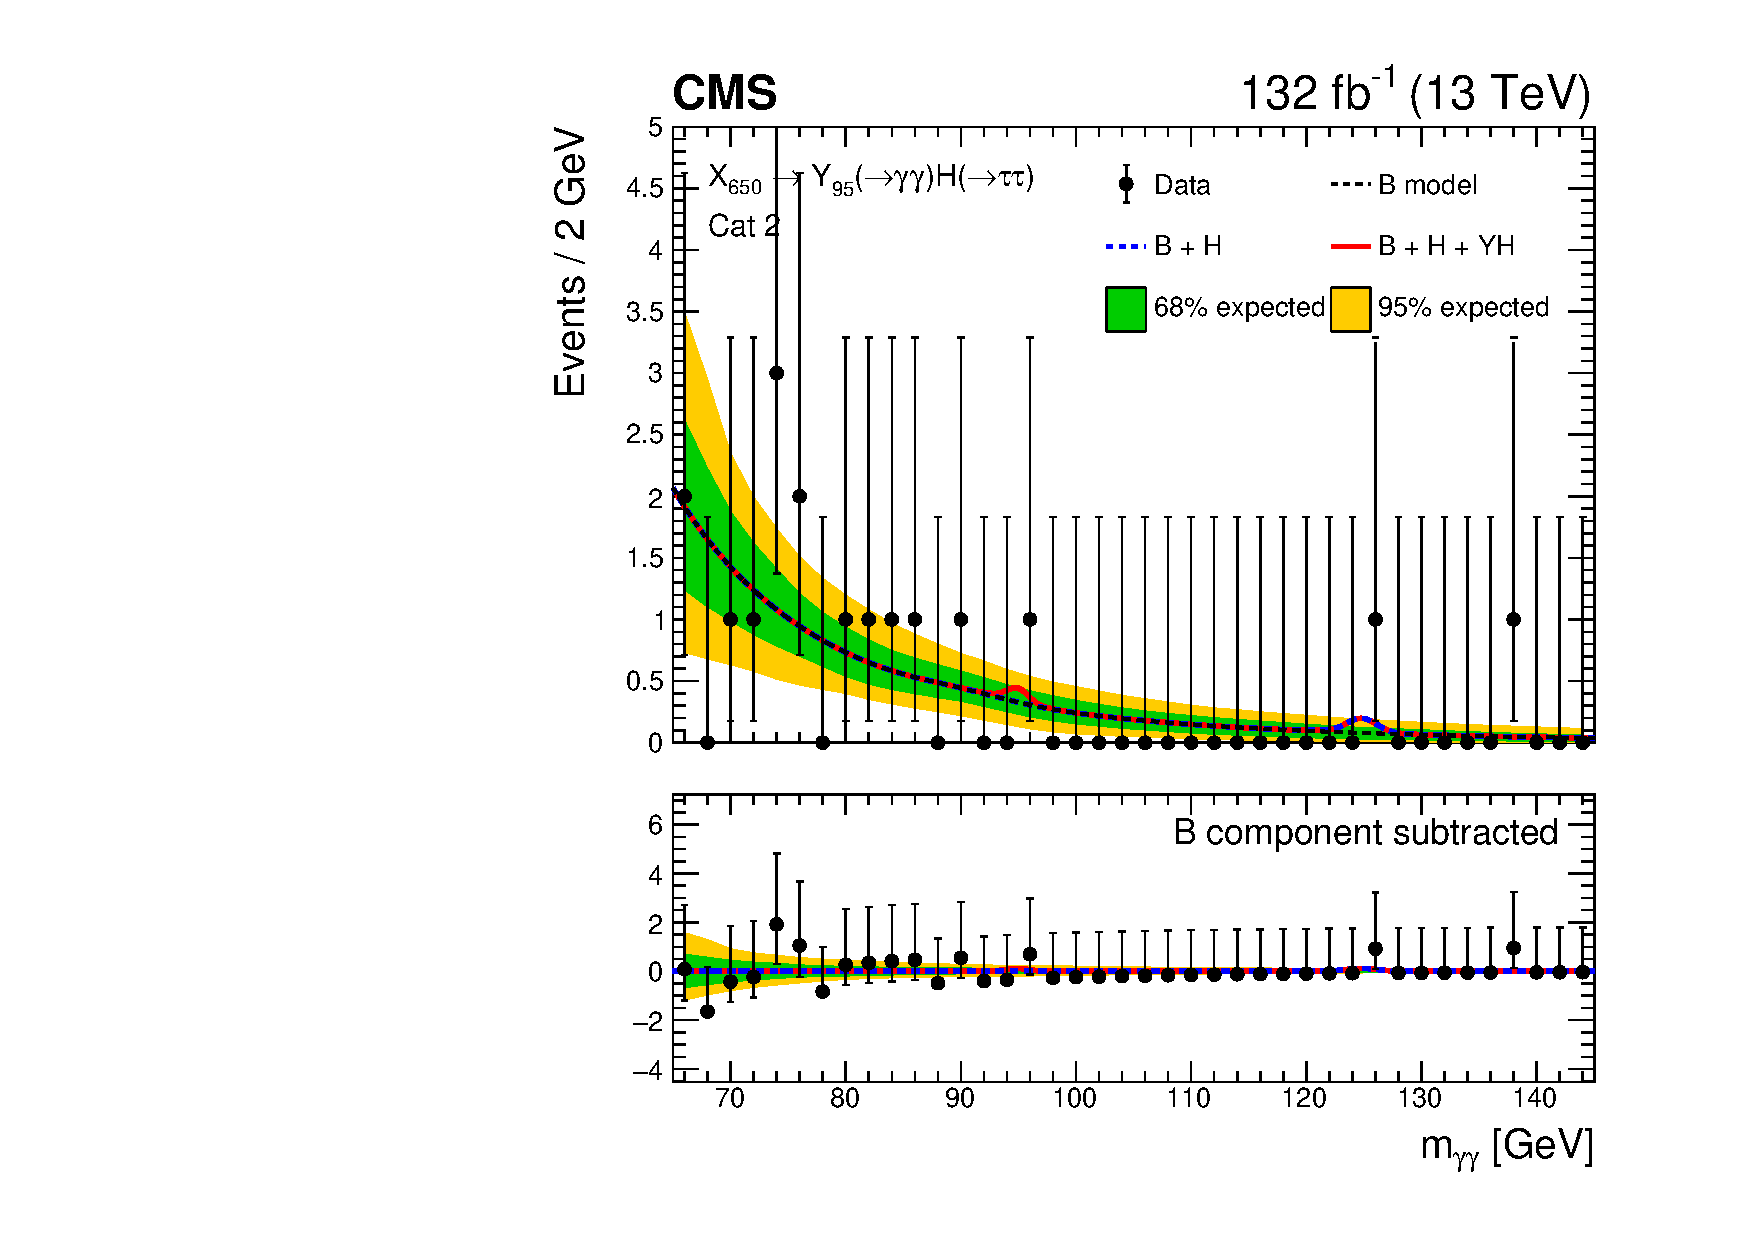
\includegraphics[width=.45\linewidth]{Figures/Dihiggs/results/sb_models/y_gg_low_mass_mx650my95/ARCGL_Y_gg_Low_Mass_mx650my100mh95_ggttresmx650my100cat2_CMS_hgg_mass_nbins40_paper.pdf}
    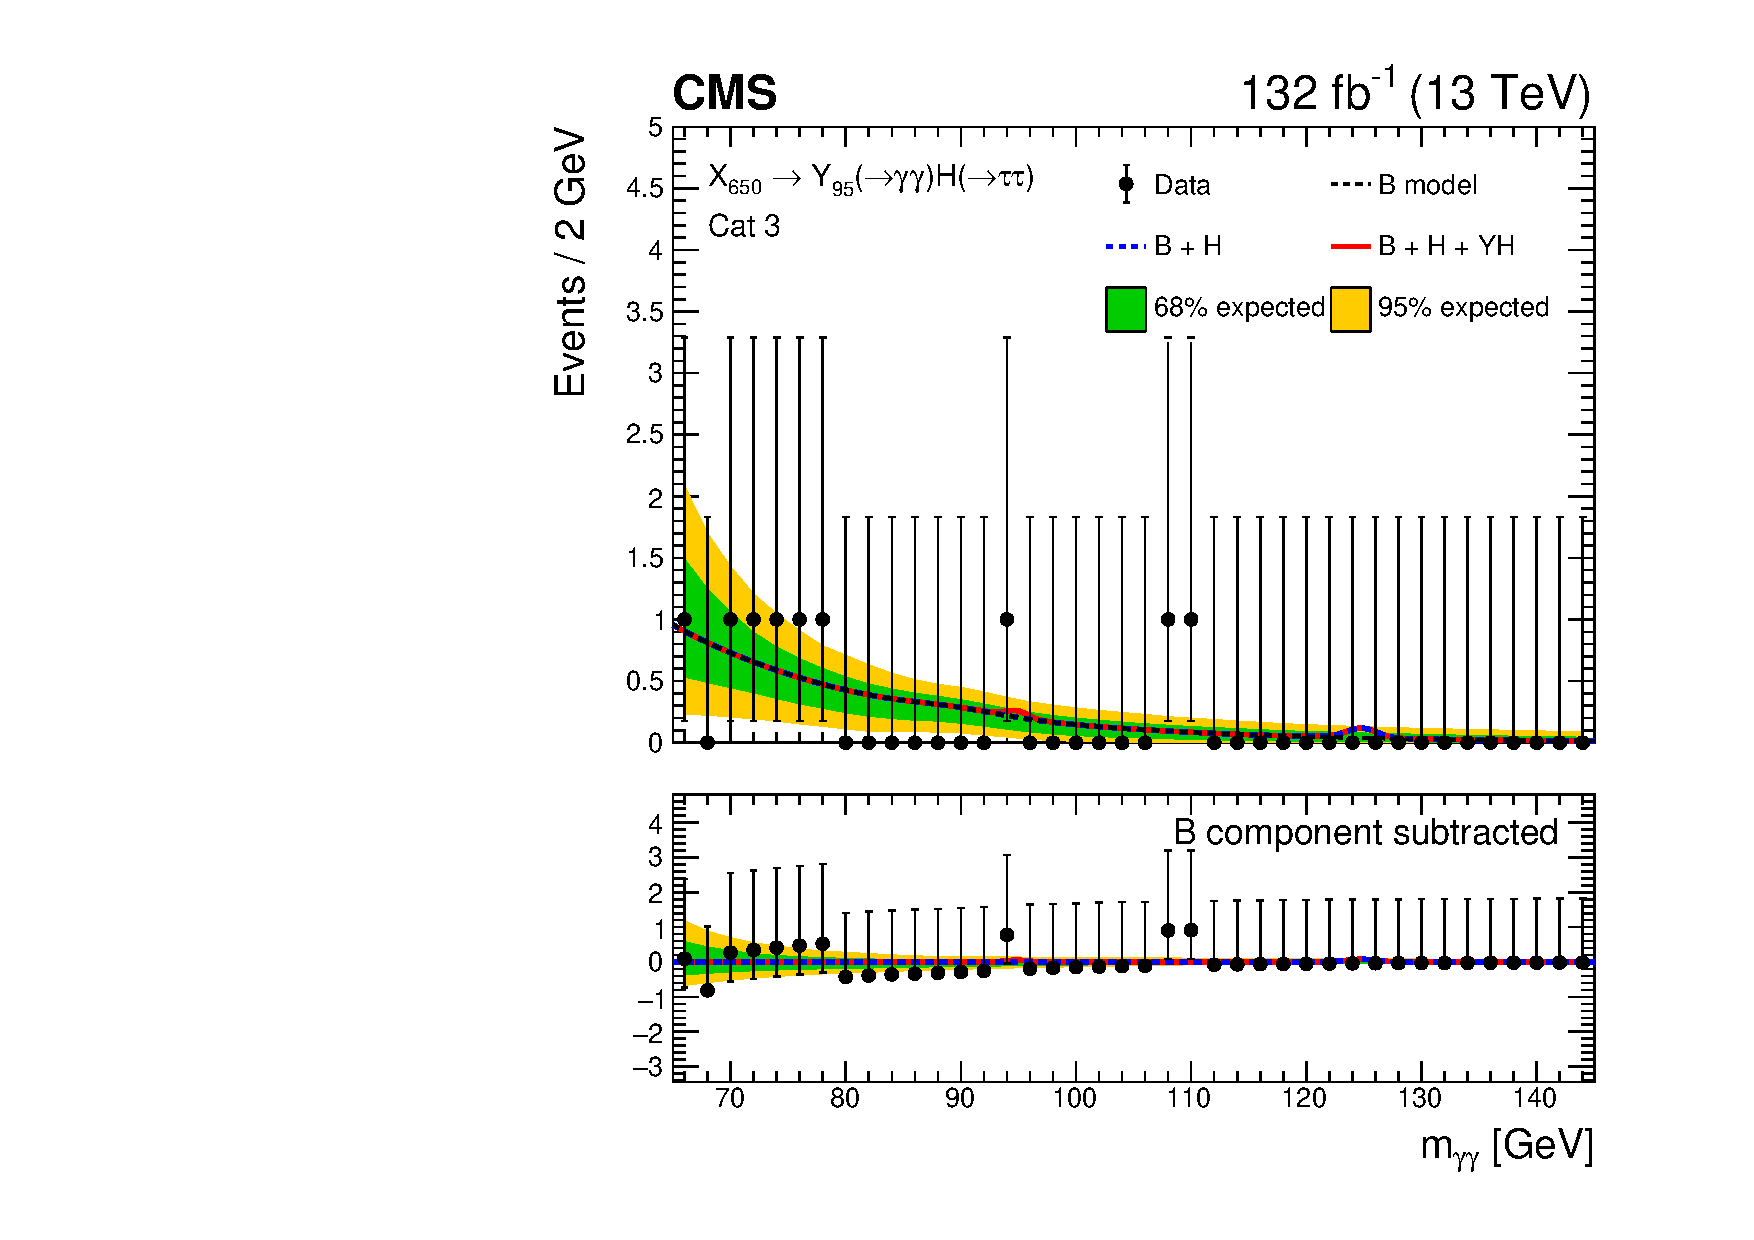
\includegraphics[width=.45\linewidth]{Figures/Dihiggs/results/sb_models/y_gg_low_mass_mx650my95/ARCGL_Y_gg_Low_Mass_mx650my100mh95_ggttresmx650my100cat3_CMS_hgg_mass_nbins40_paper.pdf}
    \caption[Signal-Plus-Background Fits to Data for Low-Mass \XYggHtt Search at $(\mX,\mY)=(650,95)$\GeV]{Distributions of \mgg in data in each analysis category corresponding to a signal region and the signal-plus-background models (red) with data (black points) in the low-mass \XYggHtt search for $(\mX,\mY)=(650,95)$\GeV. The one (green) standard deviation and two (yellow) standard deviation bands show the uncertainties in the nonresonant + DY background component of the model (black dashed line). The resonant single-Higgs background is plotted separately in blue (blue dashed line). The lower panel shows the residuals after subtraction of the nonresonant background component.}\label{fig:sbmodel_6}
\end{figure}

\begin{figure}
    \centering
    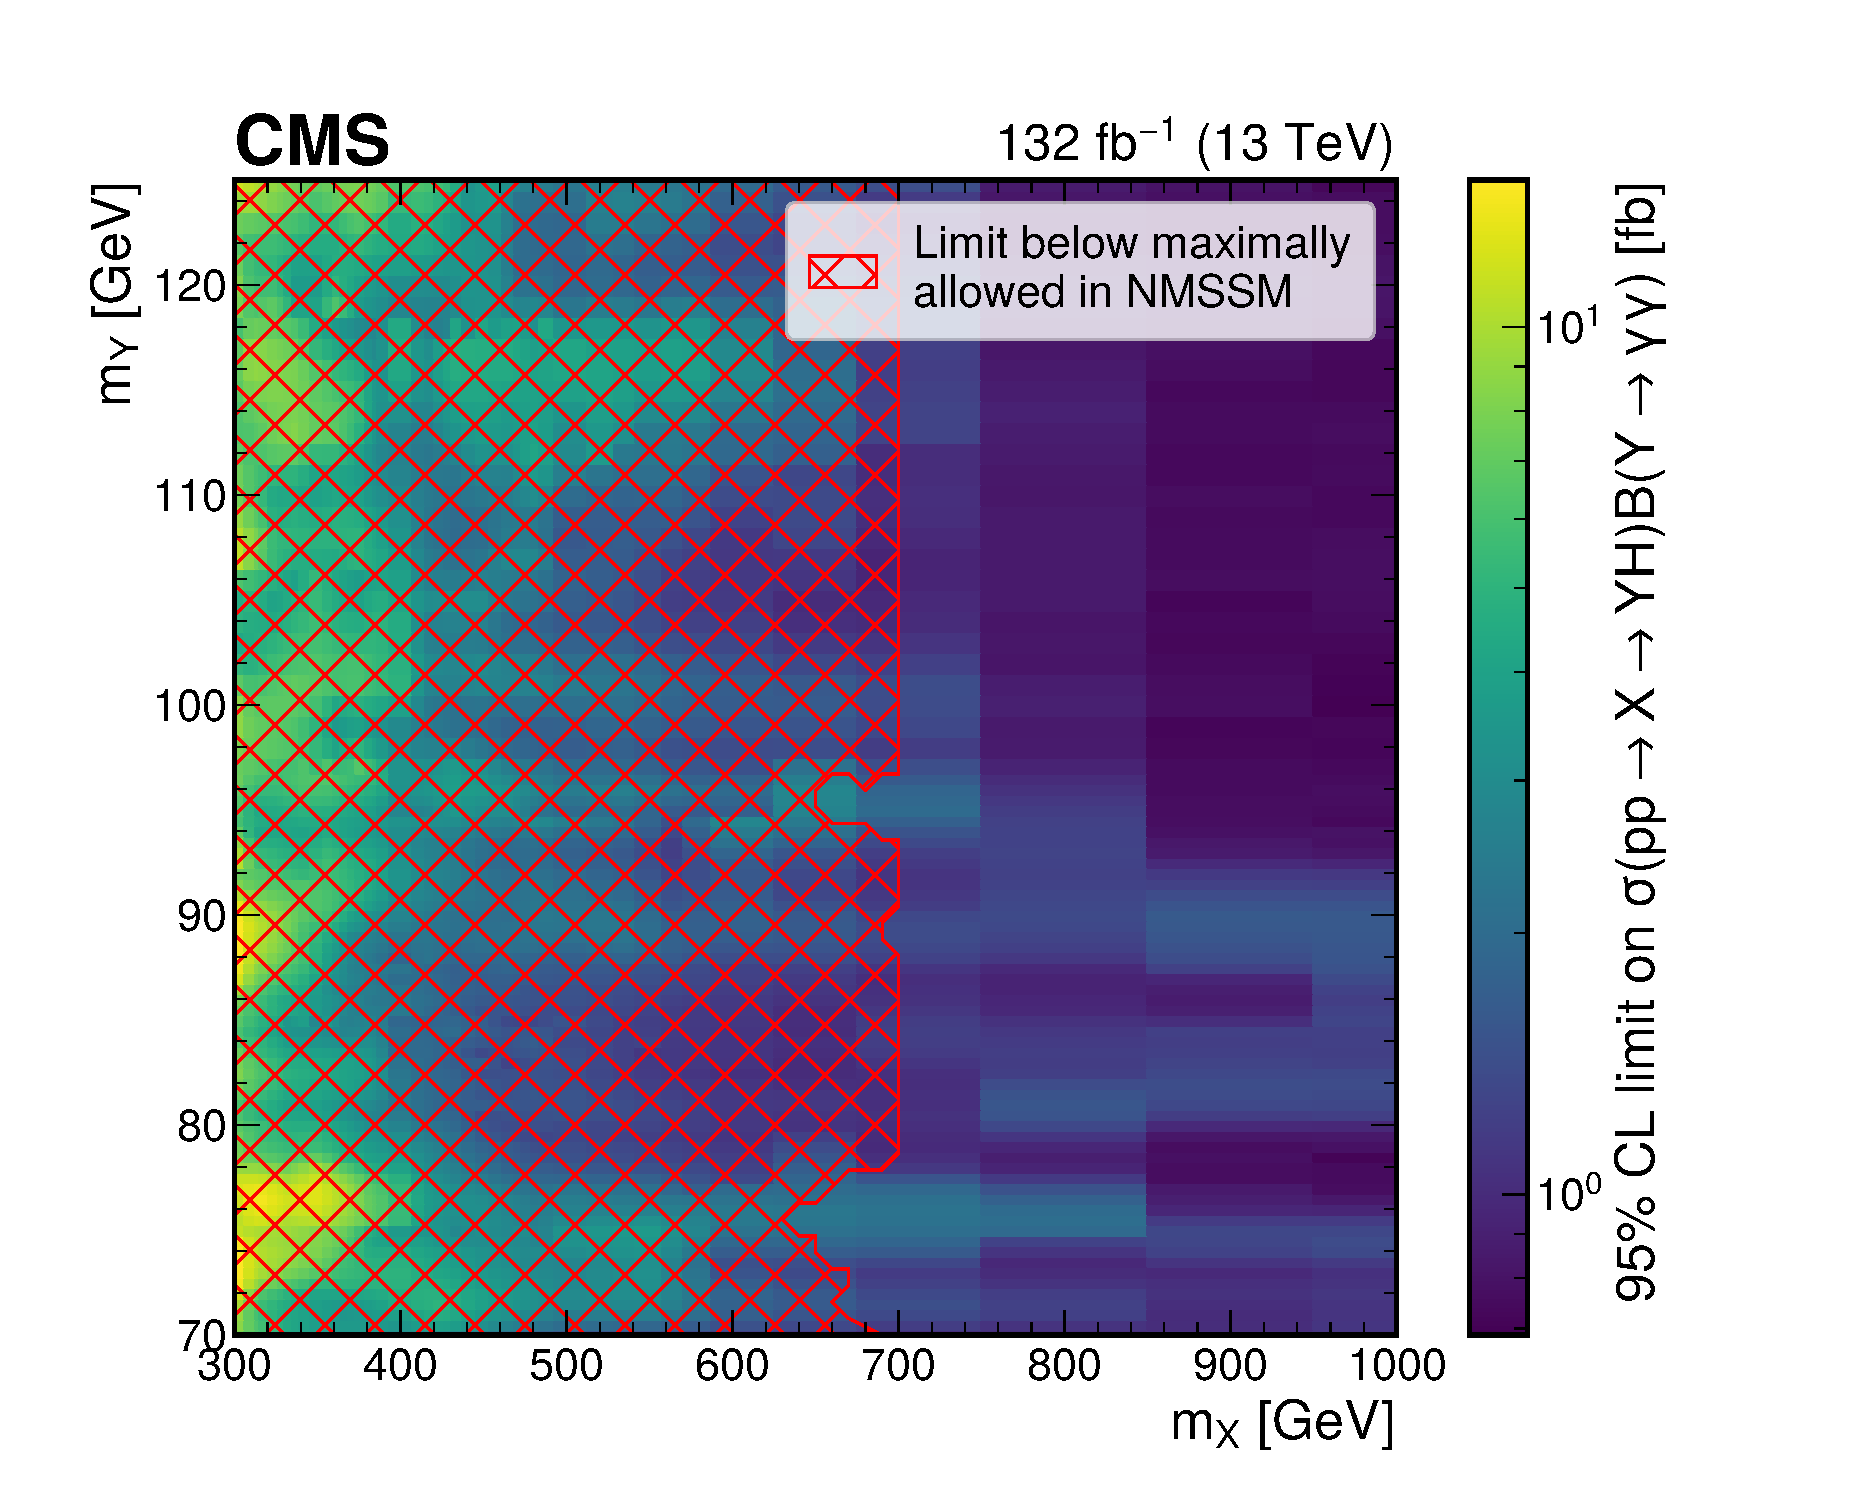
\includegraphics[width=0.8\textwidth]{Figures/Dihiggs/results/limits/limits_2d_obs_y_gg_low_mass_paper.pdf}
    \caption[Low-Mass \XYggHtt Upper Limits in the 2D $(\mX,\mY)$ Plane]{Observed 95\% CL upper limits on $\sigma(\ppXYH)\BR(\Ygg)$ in the 2D $(\mX,\mY)$ plane for the low-mass \XYggHtt search. The region of points where the observed limit is below the maximally-allowed values in the NMSSM given experimental constraints (\cref{sec:low_mass_in_NMSSM}) is indicated by the red hatching.}\label{fig:limits_2d_obs_y_gg_low_mass}
\end{figure}

\begin{figure}
    \centering
    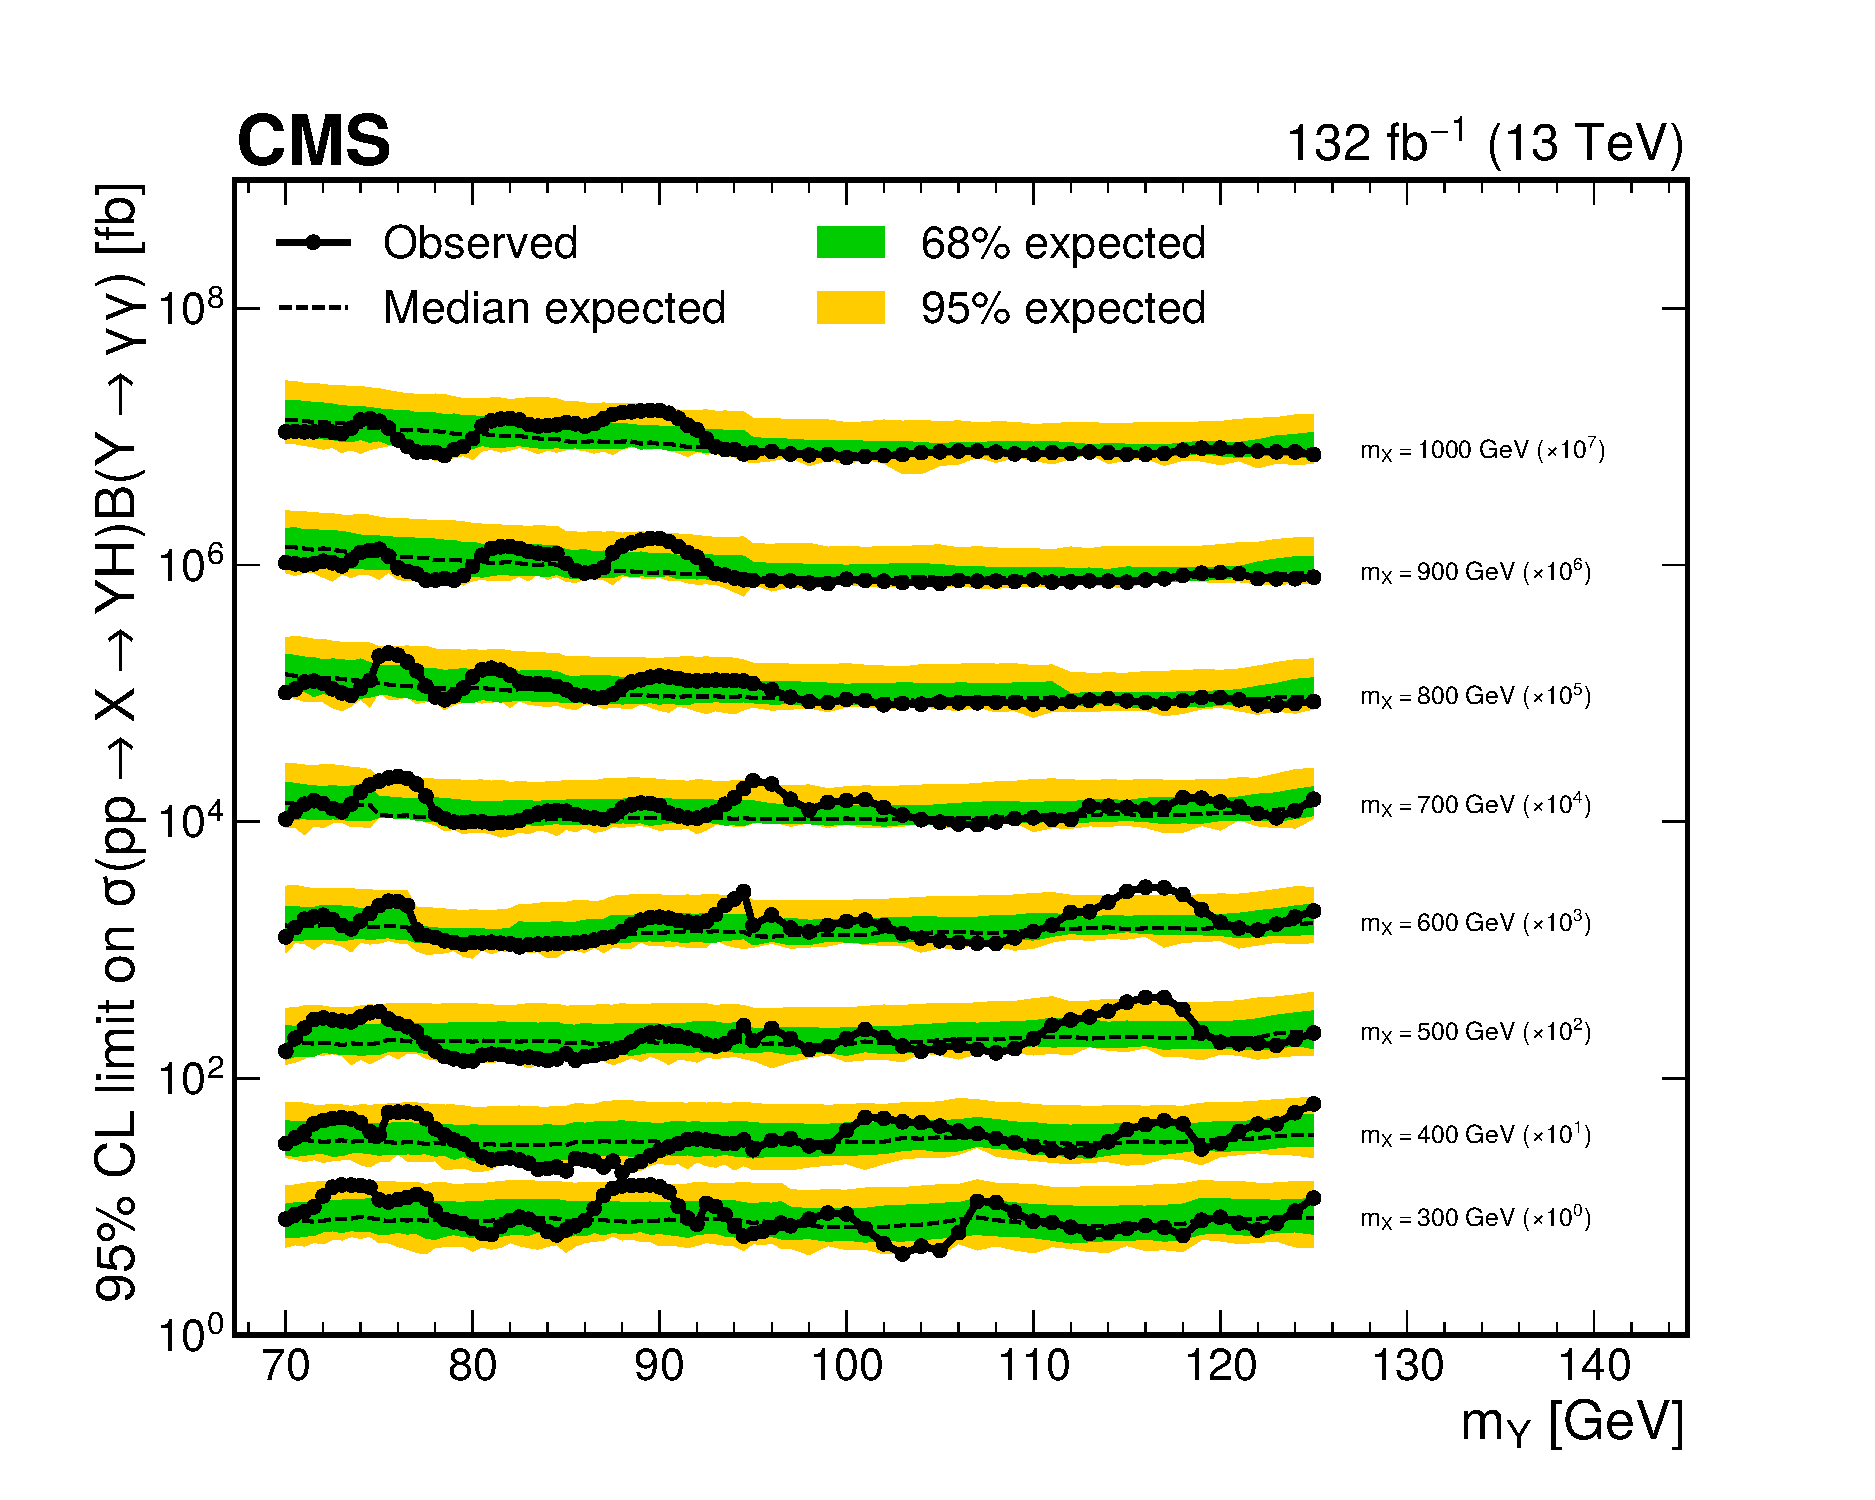
\includegraphics[width=\textwidth]{Figures/Dihiggs/results/limits/limits_stack_mx_y_gg_low_mass_paper.pdf}
    \caption[Low-Mass \XYggHtt Upper Limits in as Function of \mY in Slices of \mX]{Expected and observed 95\% CL upper limits on $\sigma(\ppXYH)\BR(\Ygg)$ for the low-mass \XYggHtt search. Limits are shown as a function of \mY for the nominal values of \mX where the limits are scaled by orders of 10 as labelled in the plot. The solid and dashed black lines represent observed and median expected limits respectively. The inner (green) band and the outer (yellow) band indicate the regions containing 68 and 95\%, respectively, of the distribution of limits expected under the background-only hypothesis.}\label{fig:limits_stack_mx_y_gg_low_mass}
\end{figure}

\begin{figure}
    \centering
    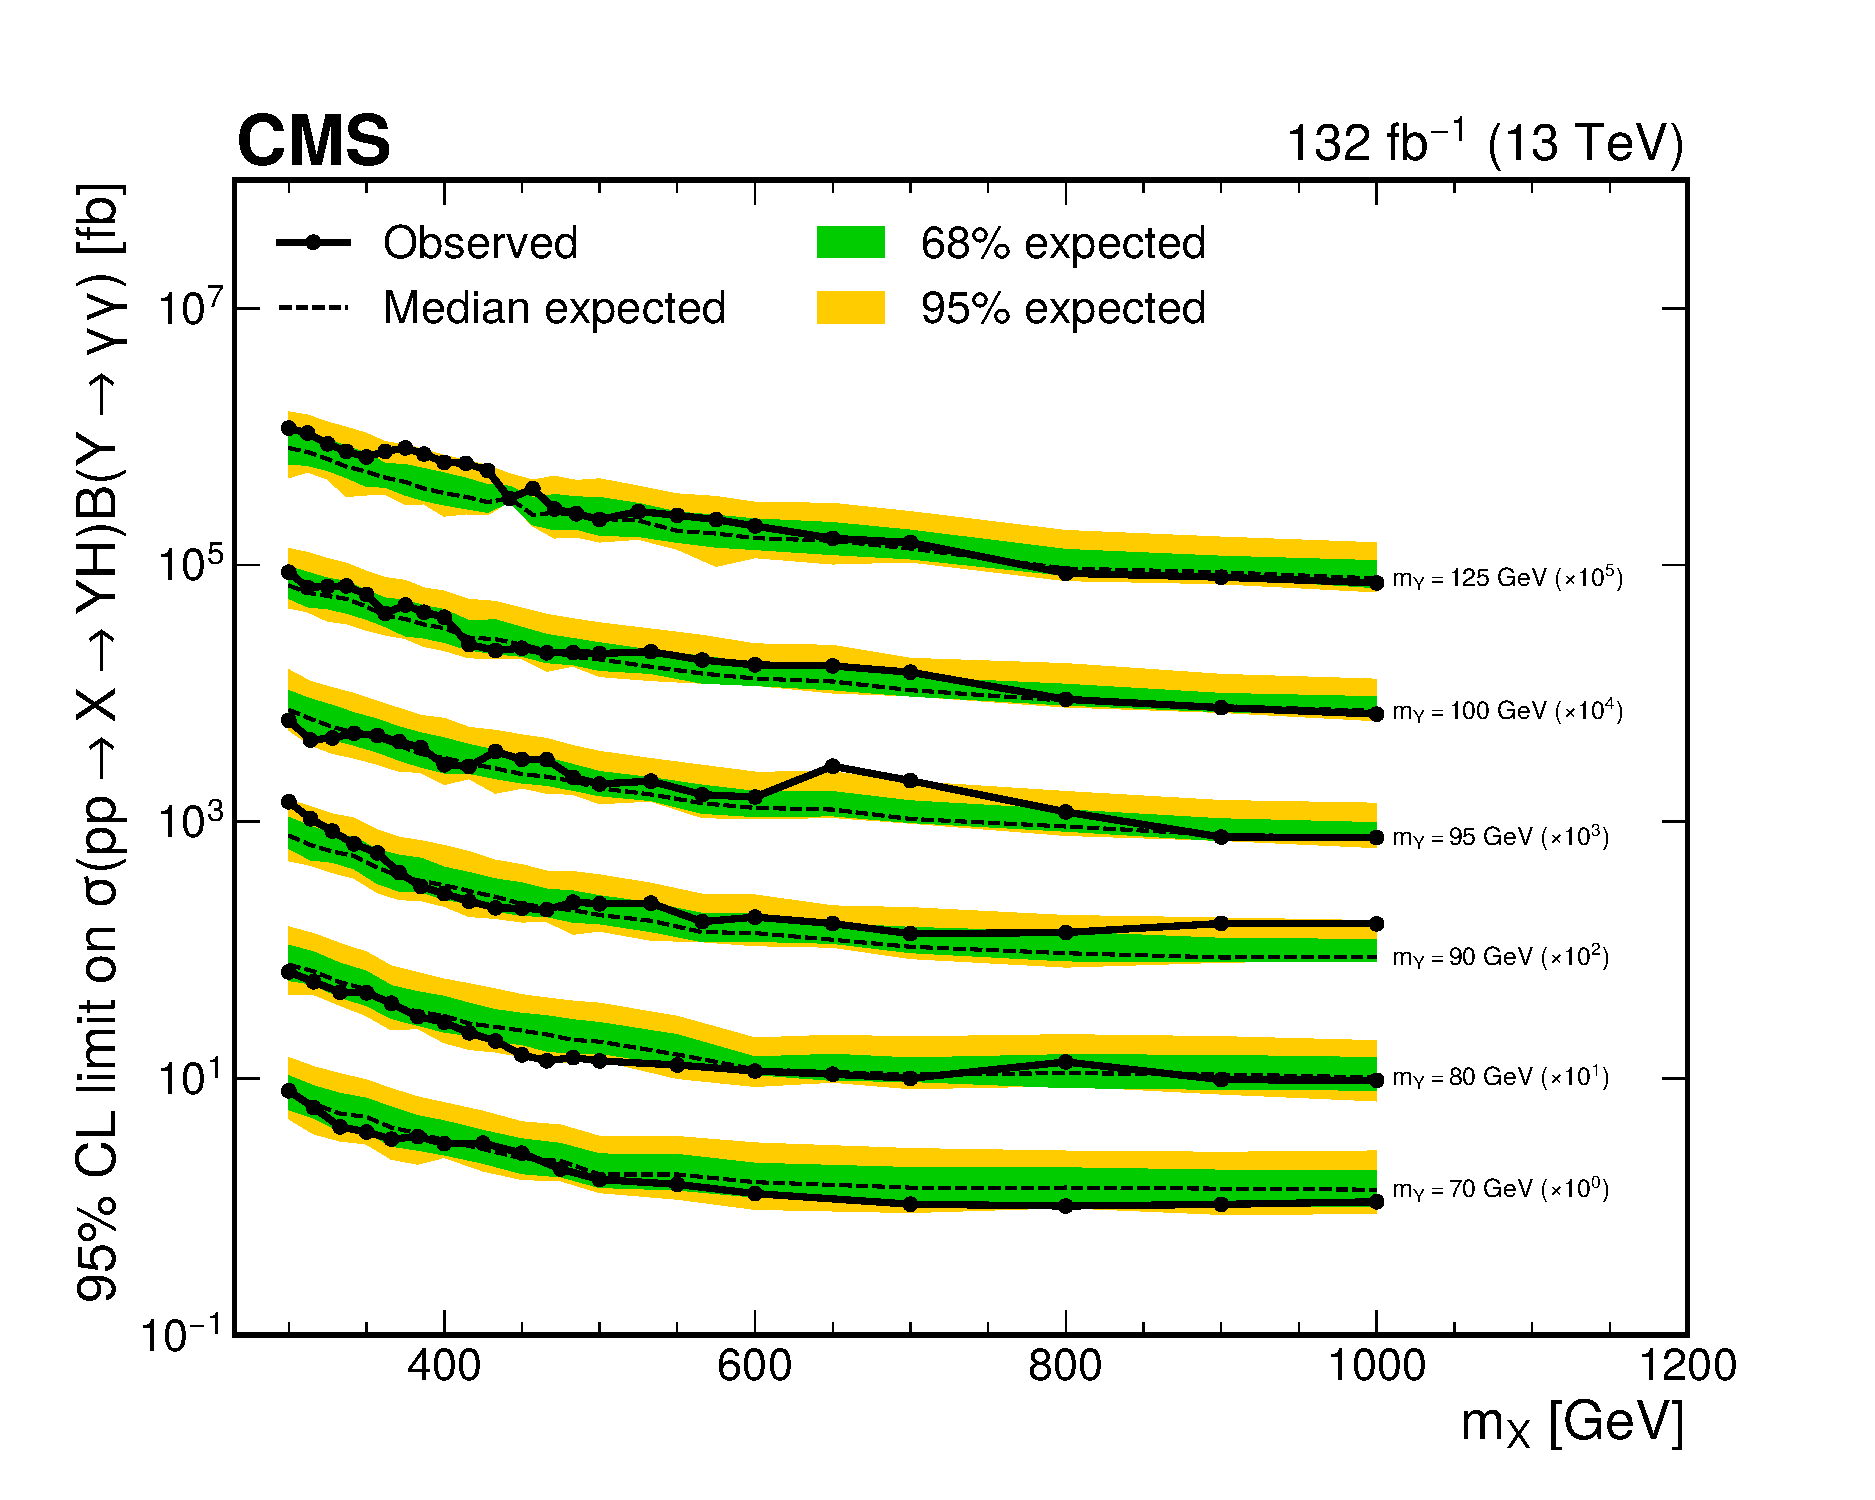
\includegraphics[width=\textwidth]{Figures/Dihiggs/results/limits/limits_stack_my_y_gg_low_mass_paper.pdf}
    \caption[Low-Mass \XYggHtt Upper Limits in as Function of \mX in Slices of \mY]{Expected and observed 95\% CL upper limits on $\sigma(\ppXYH)\BR(\Ygg)$ for the low-mass \XYggHtt search. Limits are shown as a function of \mX for the nominal values of \mY where the limits are scaled by orders of 10 as labelled in the plot. The solid and dashed black lines represent observed and median expected limits respectively. The inner (green) band and the outer (yellow) band indicate the regions containing 68 and 95\%, respectively, of the distribution of limits expected under the background-only hypothesis.}\label{fig:limits_stack_my_y_gg_low_mass}
\end{figure}

\subsection[High-Mass \texorpdfstring{\XYggHtt}{XY(tt)H(gg)} Search]{High-Mass \XYggHtt Search}\label{sec:results_y_gg_high_mass}

\Cref{fig:significance_y_gg_low_mass} shows the local significances for every mass point in the high-mass \XYggHtt search. The largest excess is seen at $(\mX,\mY)=(450,161)$\GeV, with a local significance of 3.2 standard deviations. As in the low-mass \XYggHtt search, the large number of mass points searched at leads to a large look-elsewhere effect, and the global significance is 0.3 standard deviations. The \mgg distributions in data for this mass point, and the corresponding signal-plus-background model fit, is shown in \cref{fig:sbmodel_5}. In every category, there is a small background prediction, and at least one event near the signal peak.  

The observed 95\% CL upper limits on $\sigma(\ppXYH)\BR(\Ygg)$ for the high-mass \XYggHtt search are shown in a 2D heatmap in \cref{fig:limits_2d_obs_y_gg_high_mass}, and the expected and observed limits are shown in slices of \mX and \mY in \cref{fig:limits_stack_mx_y_gg_high_mass,fig:limits_stack_my_y_gg_high_mass}, respectively, where the slices are taken at the nominal mass points. Compared to the other \XYH searches, there is a greater dependence of \mY on the limits, where the expected limits tend to increase with \mY. This can be explained by the preselection signal efficiencies (\cref{fig:presel_eff_xyh}) which see a similar trend in \mY. The observed (expected) upper limits vary between 0.64--10\fb (0.70--7.6\fb), depending on the mass point.

\vspace{\fill}

\begin{figure}[h]
    \centering
    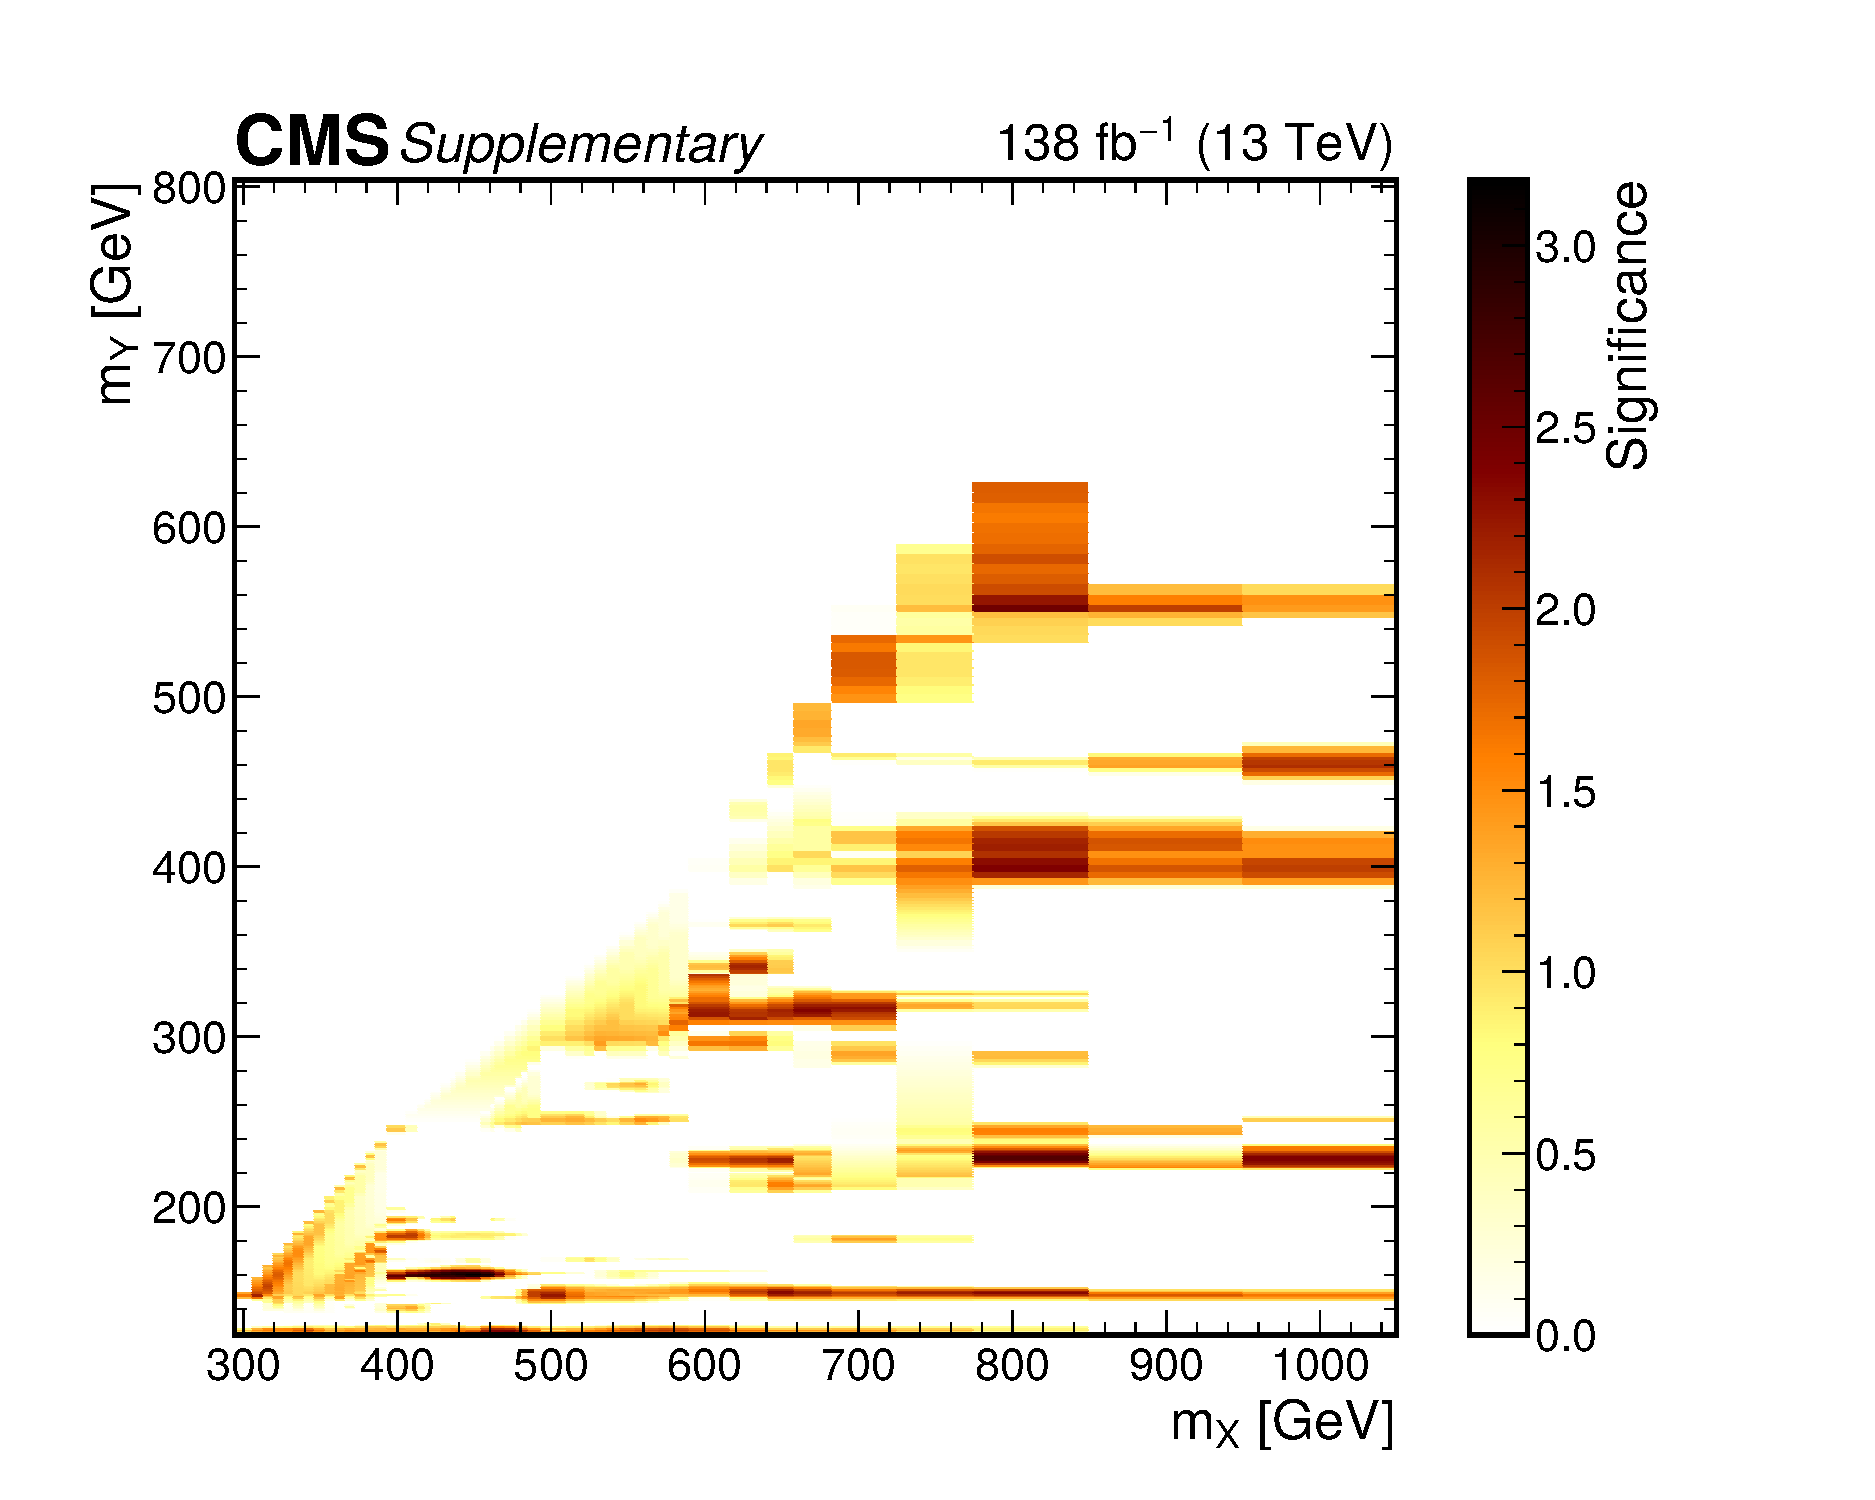
\includegraphics[width=0.8\textwidth]{Figures/Dihiggs/results/significances/significance_y_gg_high_mass_supplementary.pdf}
    \caption[High-Mass \XYggHtt Observed Local Significances]{Observed local significances in the 2D $(\mX,\mY)$ plane for the high-mass \XYggHtt search.}\label{fig:significance_y_gg_high_mass}
\end{figure}

\begin{figure}
    \centering
    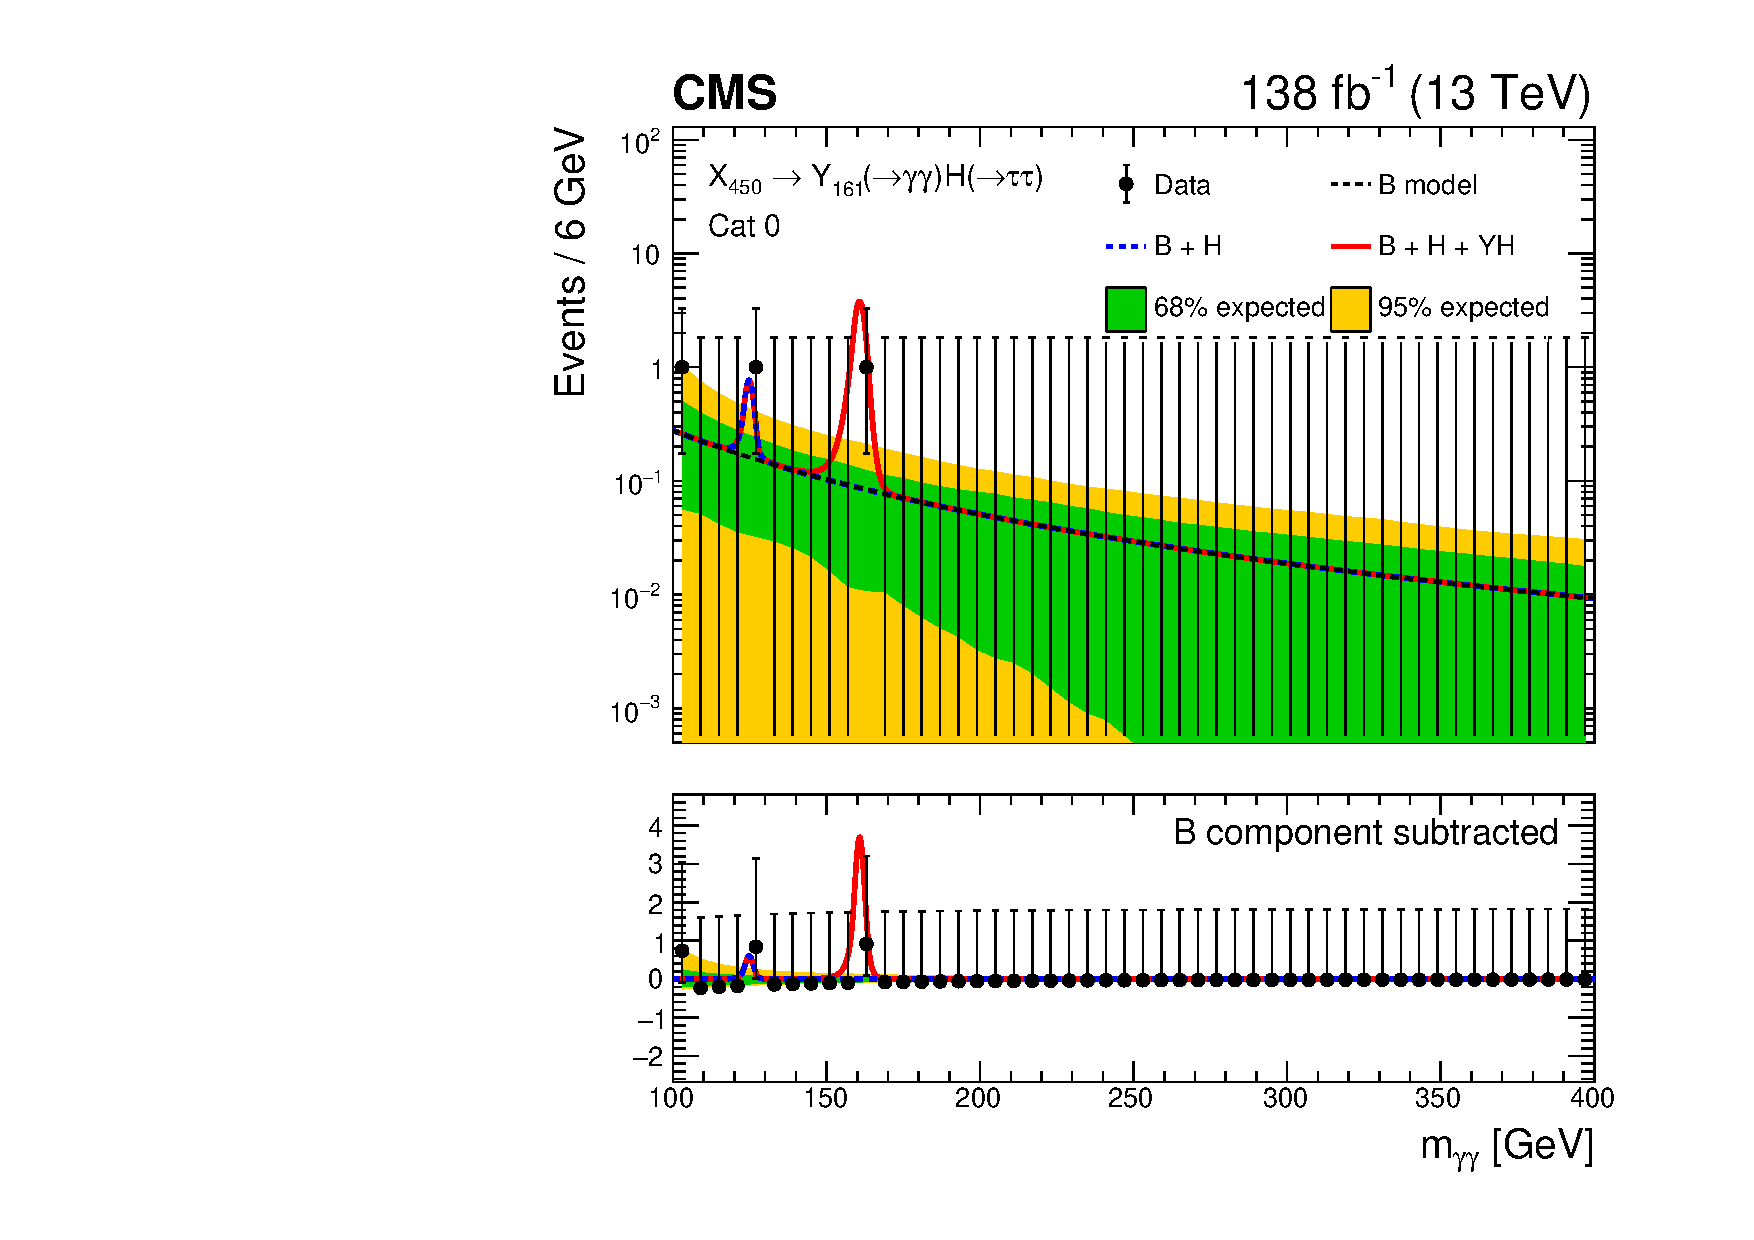
\includegraphics[width=.45\linewidth]{Figures/Dihiggs/results/sb_models/y_gg_high_mass/ARCGL_Y_gg_High_Mass_mx450my164mh161_ggttresmx450my164cat0_CMS_hgg_mass_nbins50_paper.pdf}
    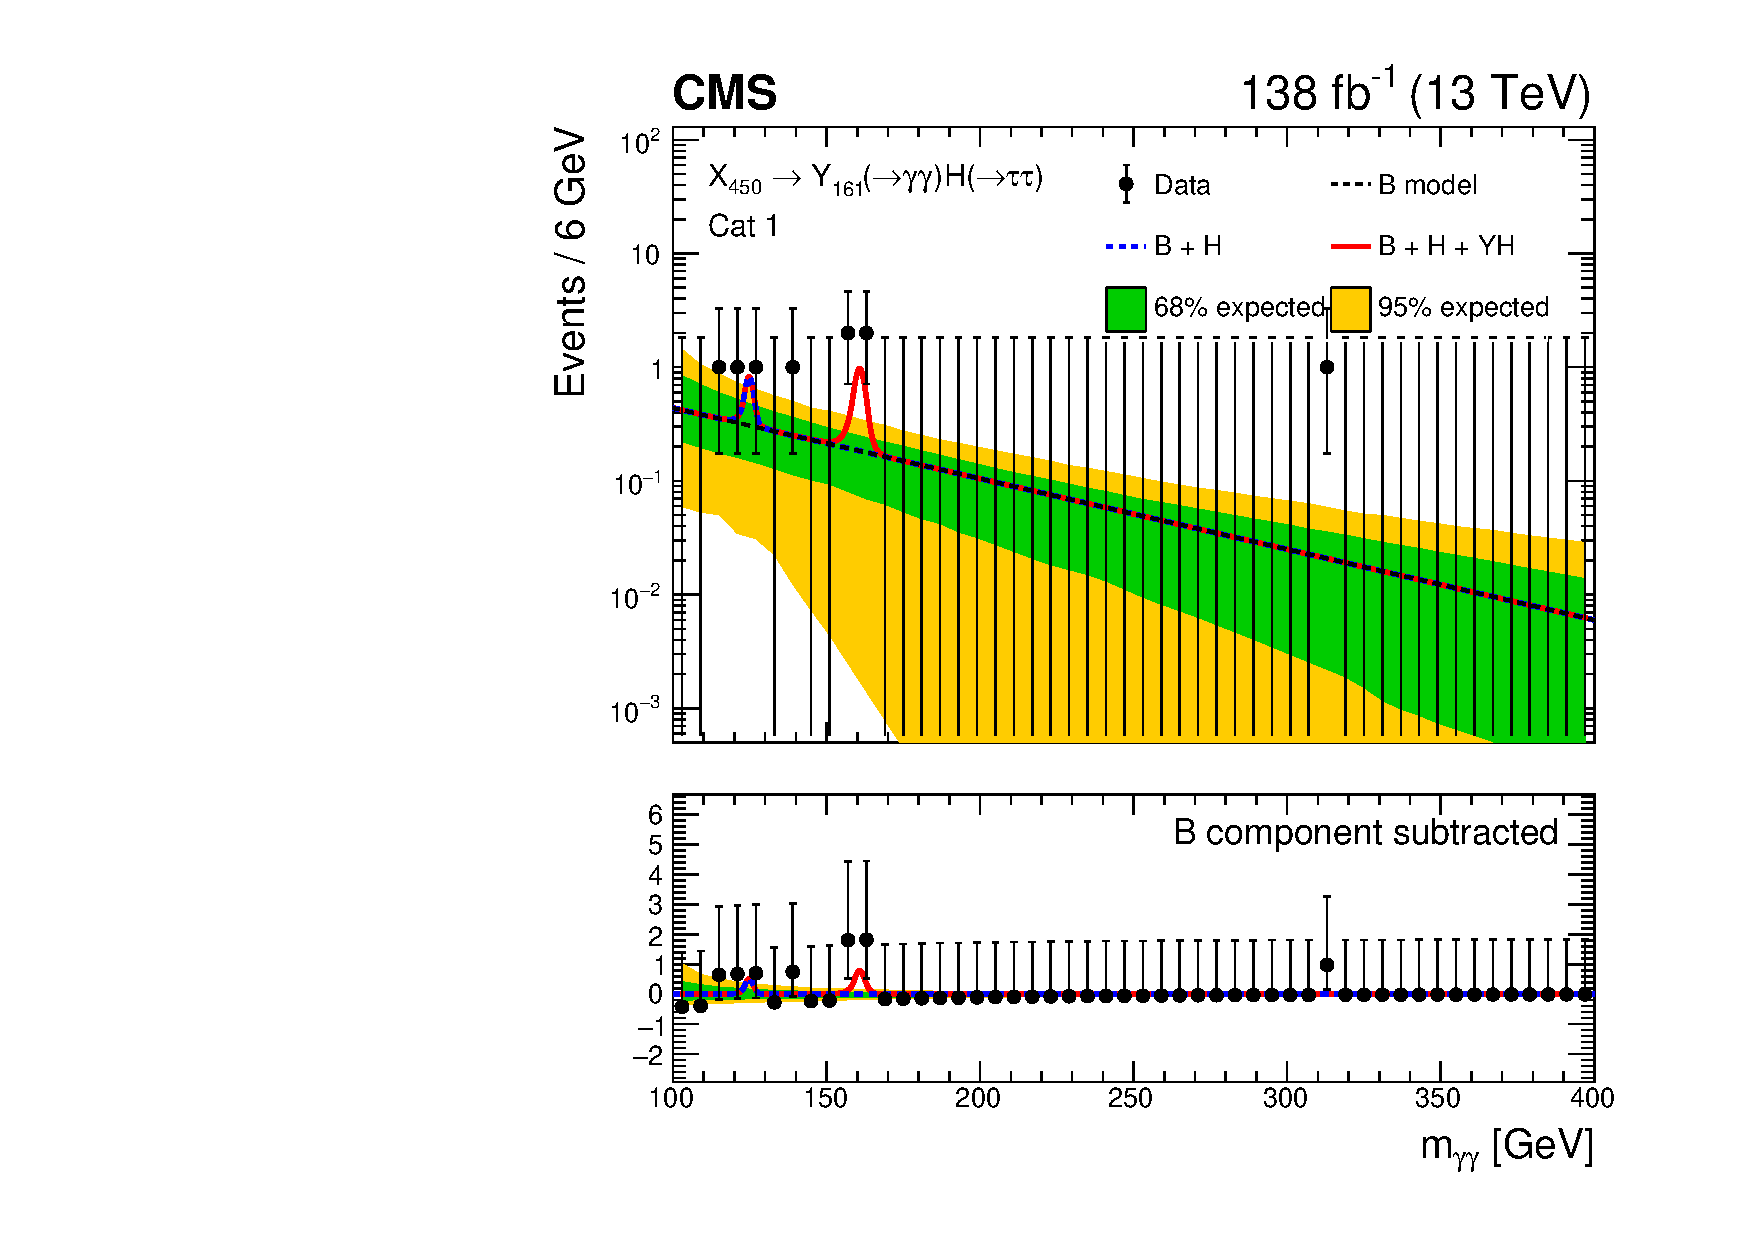
\includegraphics[width=.45\linewidth]{Figures/Dihiggs/results/sb_models/y_gg_high_mass/ARCGL_Y_gg_High_Mass_mx450my164mh161_ggttresmx450my164cat1_CMS_hgg_mass_nbins50_paper.pdf}
    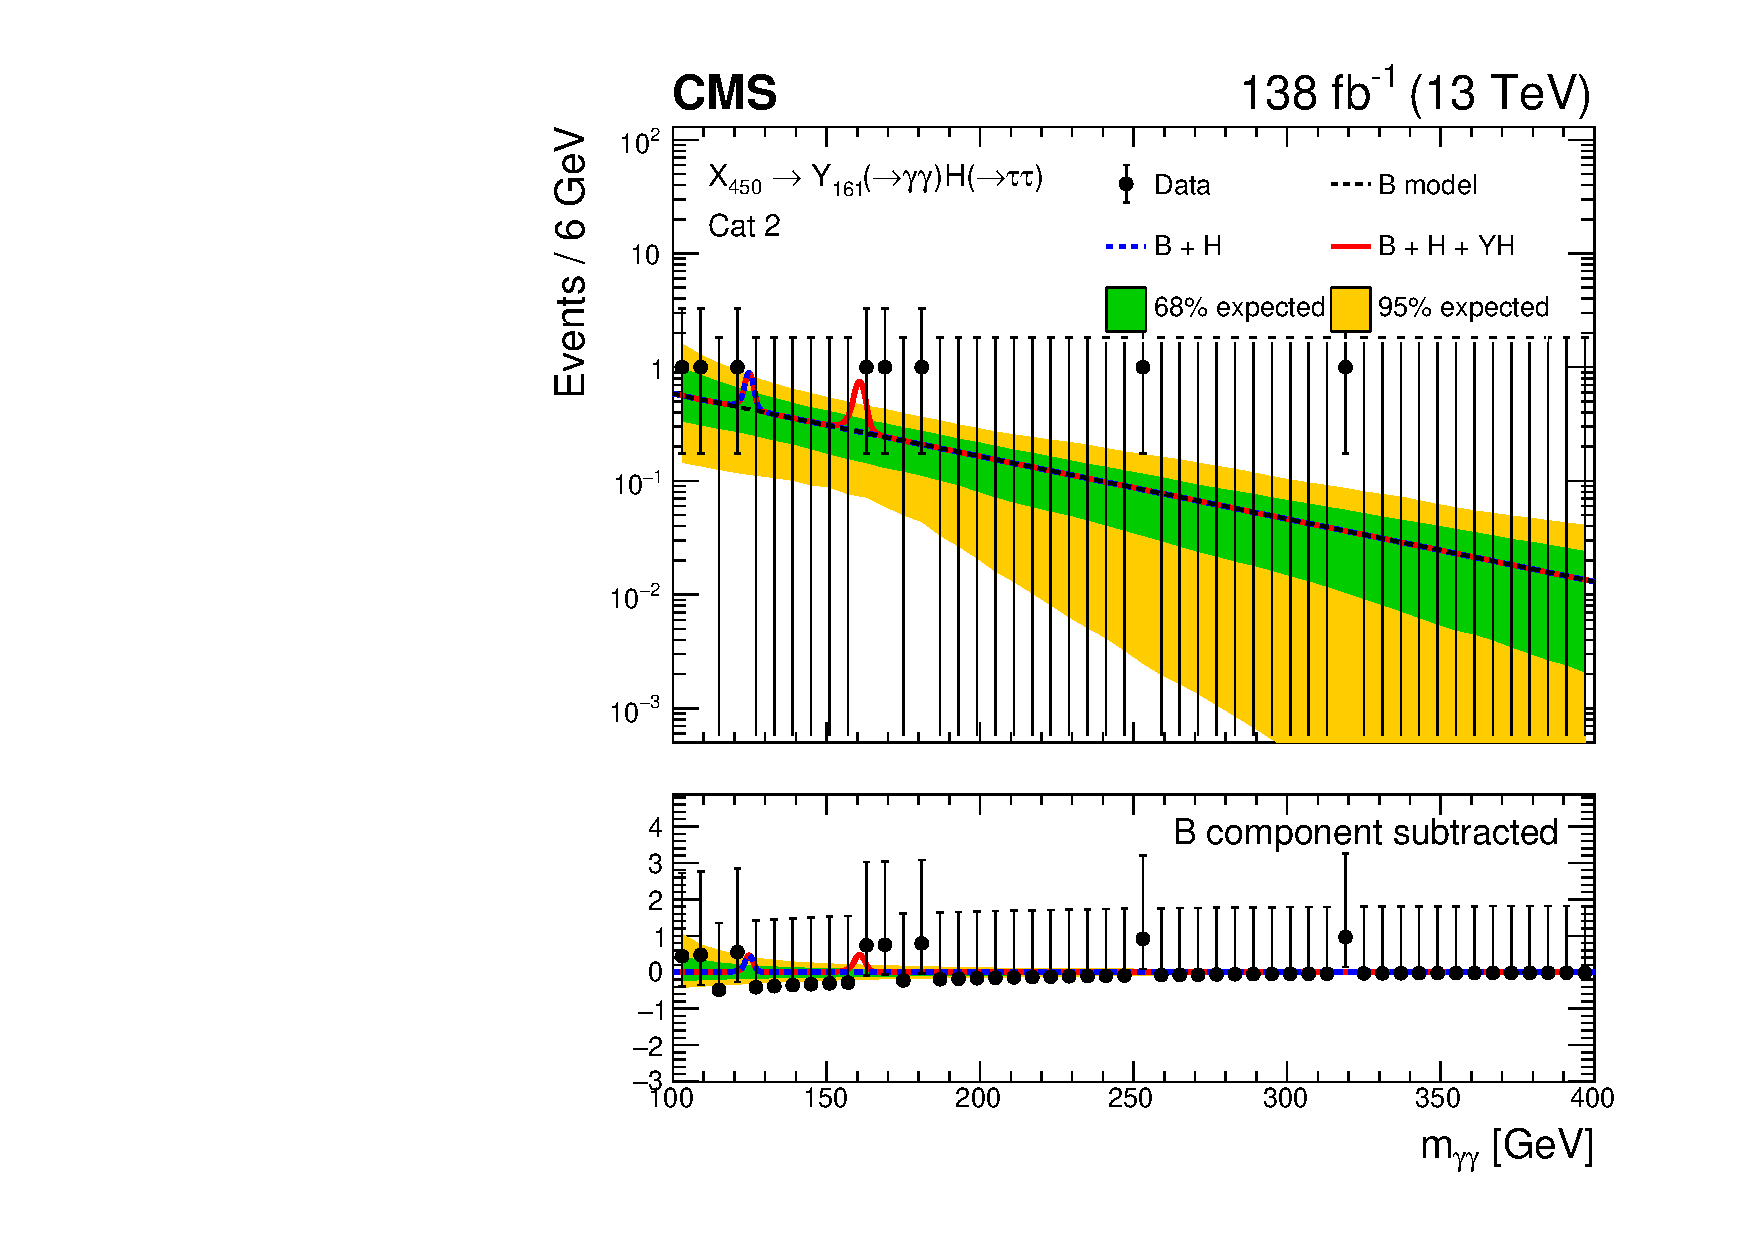
\includegraphics[width=.45\linewidth]{Figures/Dihiggs/results/sb_models/y_gg_high_mass/ARCGL_Y_gg_High_Mass_mx450my164mh161_ggttresmx450my164cat2_CMS_hgg_mass_nbins50_paper.pdf}
    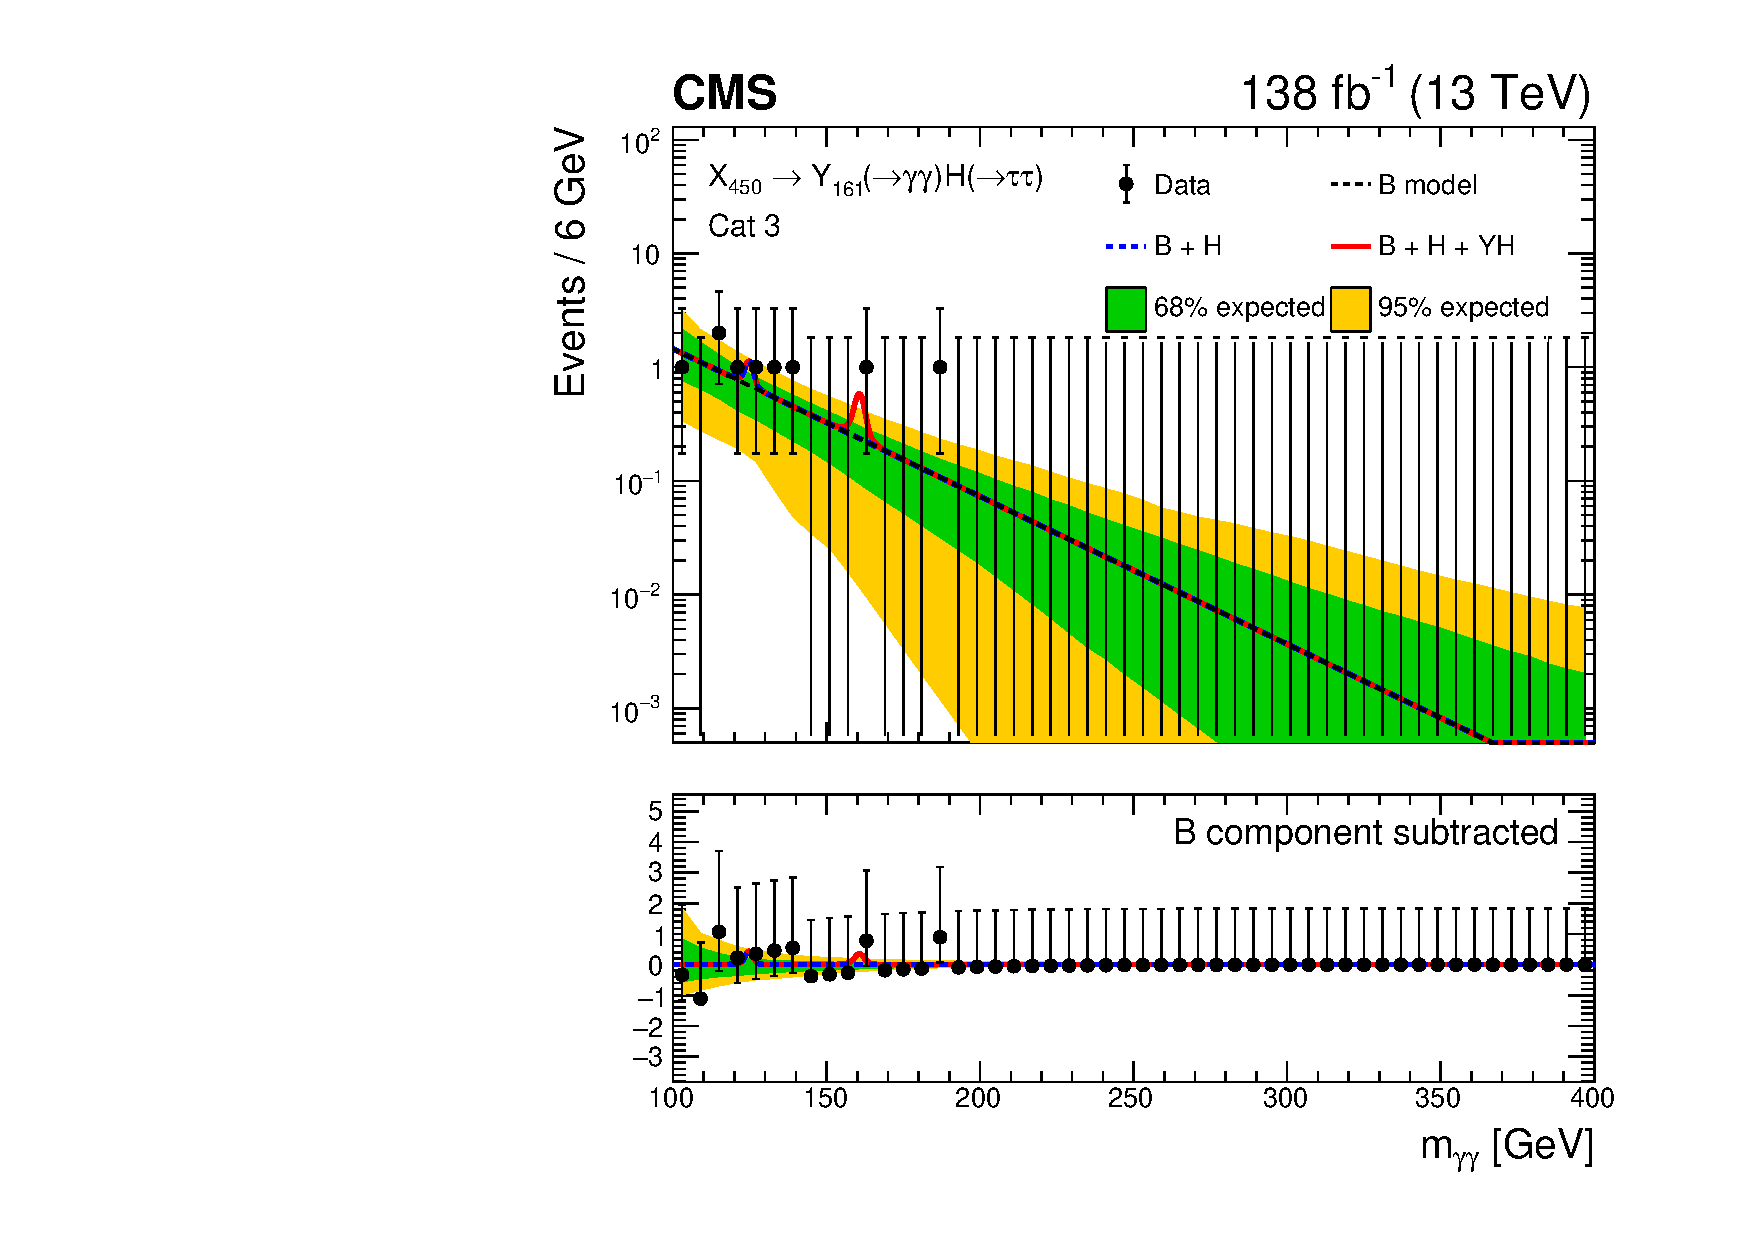
\includegraphics[width=.45\linewidth]{Figures/Dihiggs/results/sb_models/y_gg_high_mass/ARCGL_Y_gg_High_Mass_mx450my164mh161_ggttresmx450my164cat3_CMS_hgg_mass_nbins50_paper.pdf}
    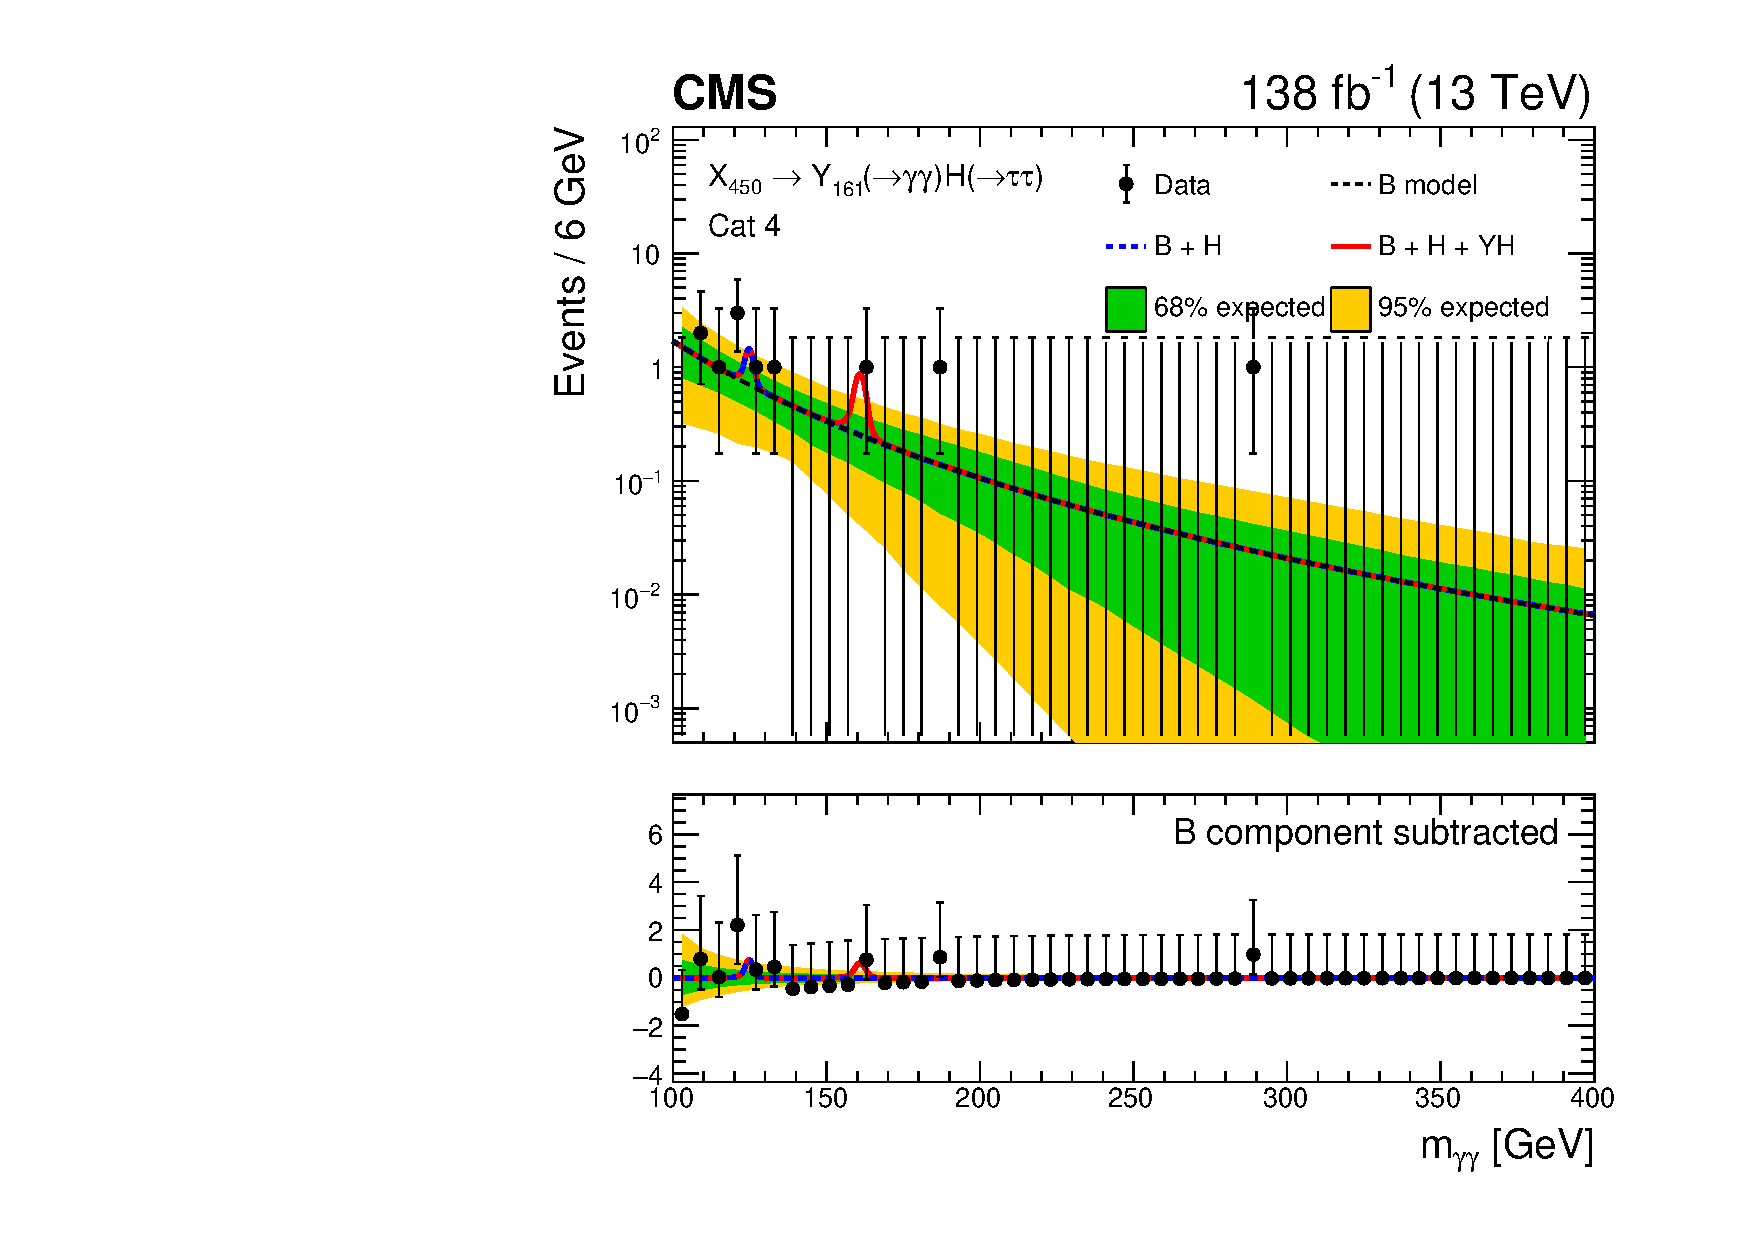
\includegraphics[width=.45\linewidth]{Figures/Dihiggs/results/sb_models/y_gg_high_mass/ARCGL_Y_gg_High_Mass_mx450my164mh161_ggttresmx450my164cat4_CMS_hgg_mass_nbins50_paper.pdf}
    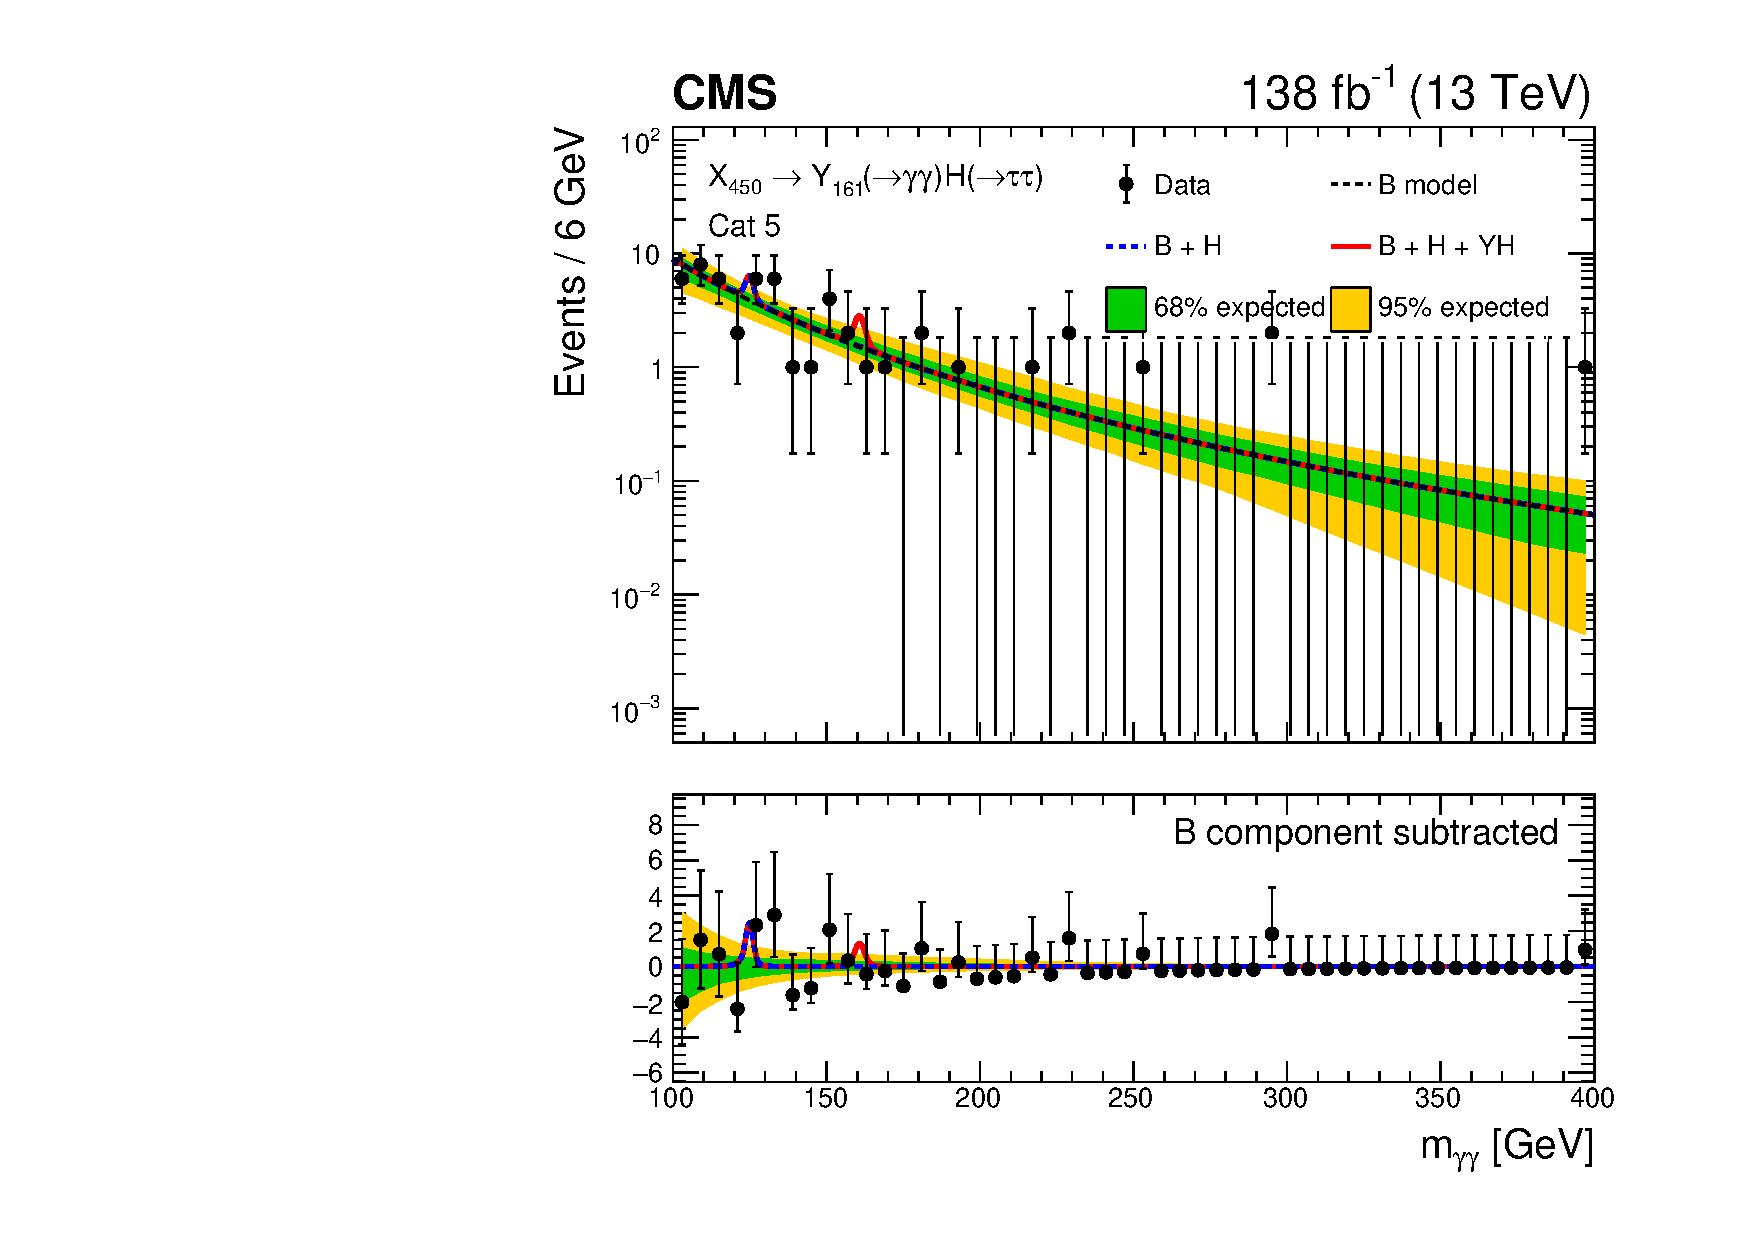
\includegraphics[width=.45\linewidth]{Figures/Dihiggs/results/sb_models/y_gg_high_mass/ARCGL_Y_gg_High_Mass_mx450my164mh161_ggttresmx450my164cat5_CMS_hgg_mass_nbins50_paper.pdf}
    \caption[Signal-Plus-Background Fits to Data for High-Mass \XYggHtt Search at $(\mX,\mY)=(462,161)$\GeV]{Distributions of \mgg in data in each analysis category and the signal-plus-background models (red) with data (black points) in the high-mass \XYggHtt search for $(\mX,\mY)=(462,161)$\GeV. The one (green) standard deviation and two (yellow) standard deviation bands show the uncertainties in the nonresonant background component of the model (black dashed line). The resonant single-Higgs background is plotted separately in blue (blue dashed line). The lower panel shows the residuals after subtraction of the nonresonant background component.}\label{fig:sbmodel_5}
\end{figure}


\begin{figure}
    \centering
    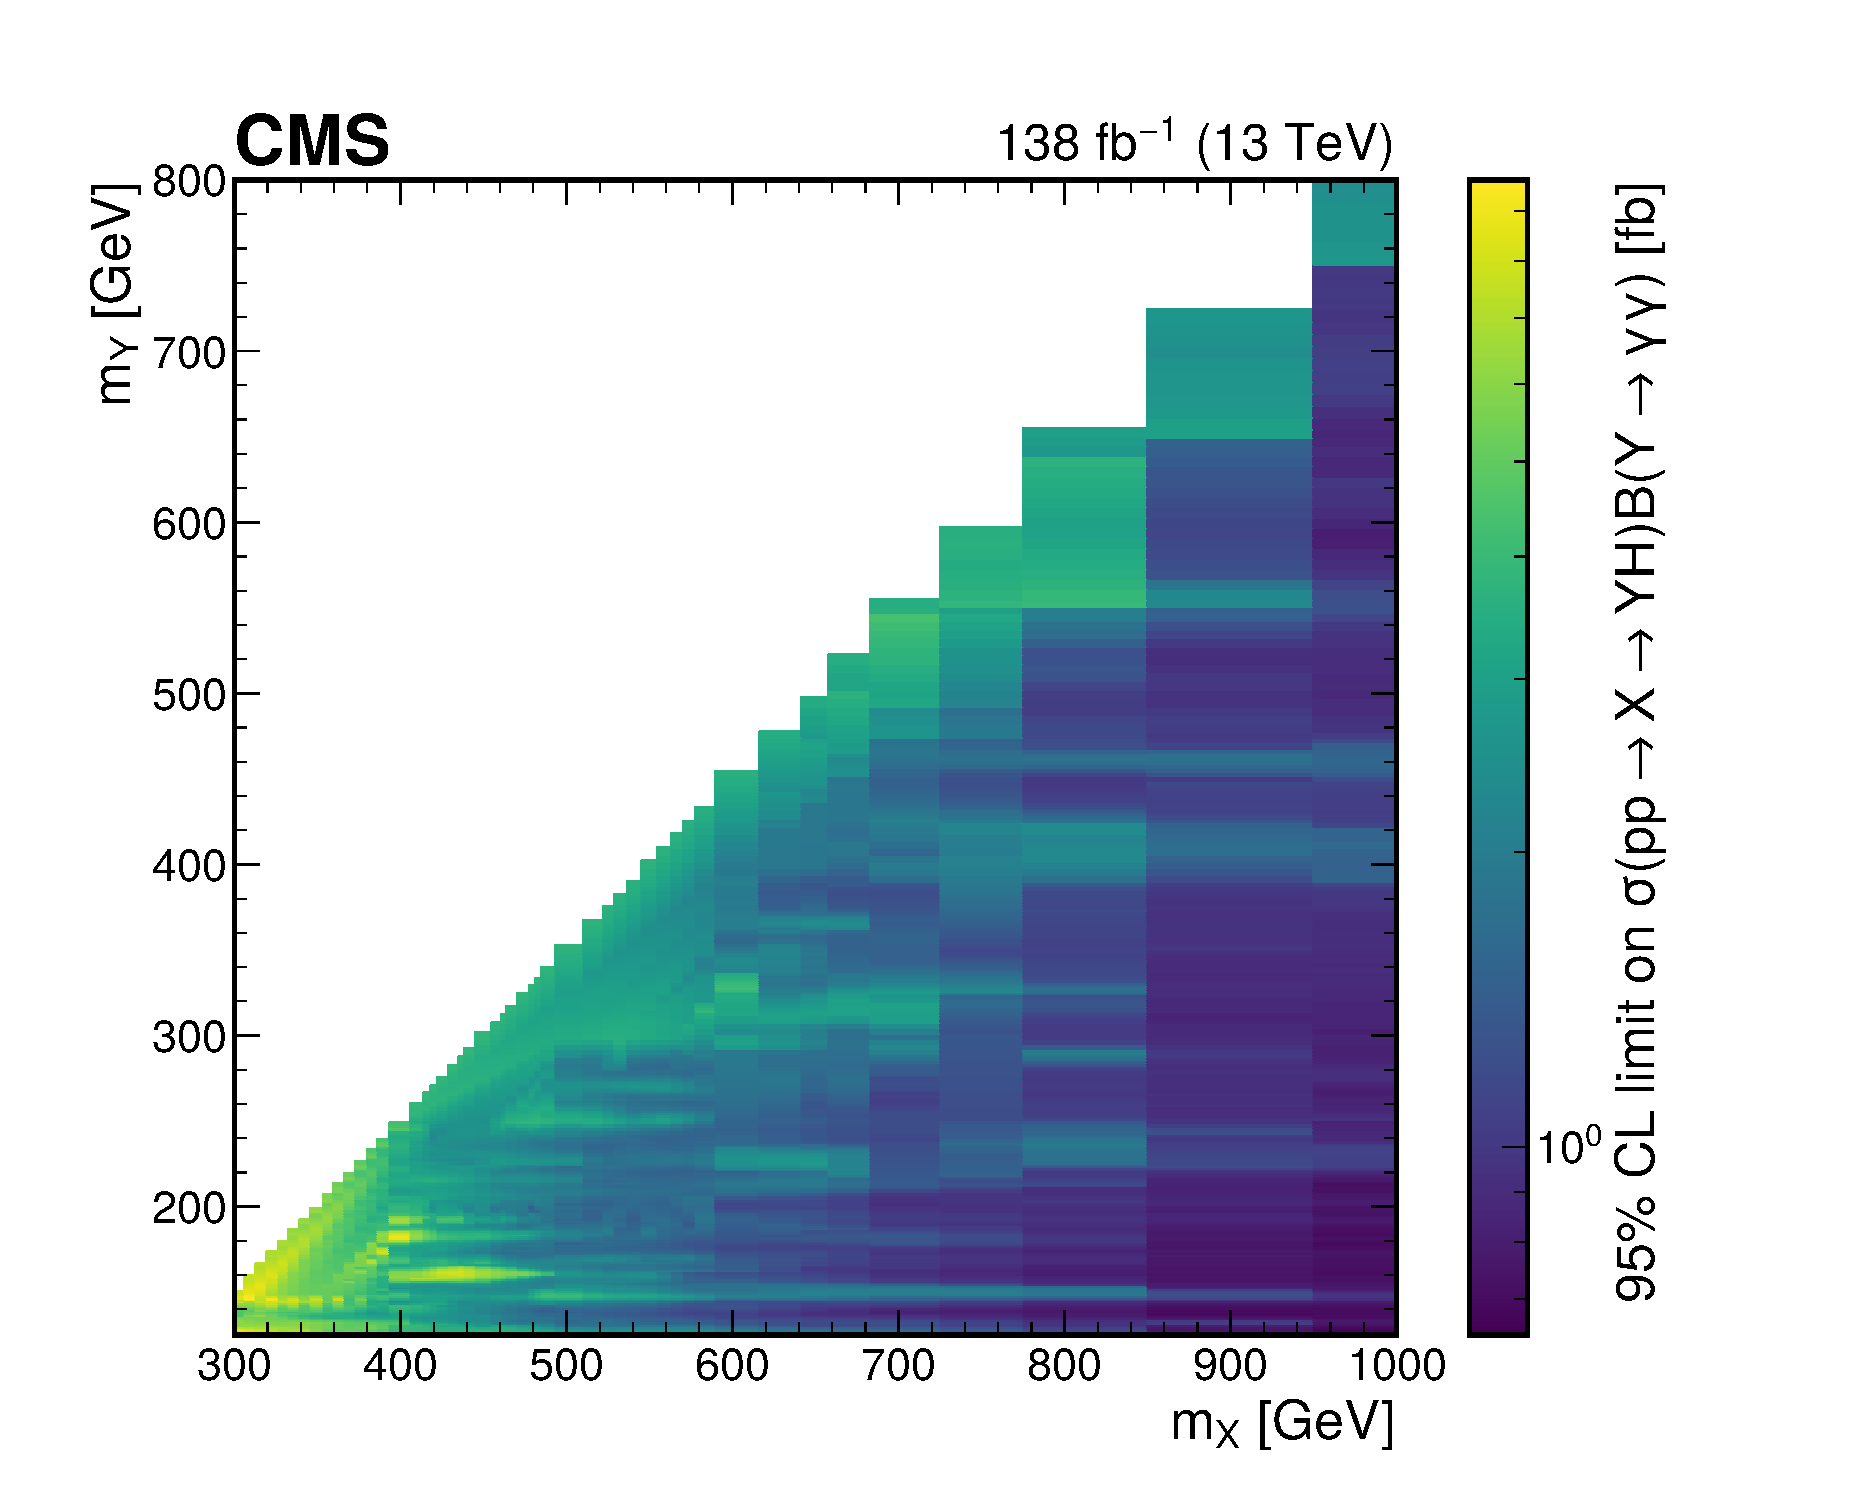
\includegraphics[width=0.8\textwidth]{Figures/Dihiggs/results/limits/limits_2d_obs_y_gg_high_mass_paper.pdf}
    \caption[High-Mass \XYggHtt Upper Limits in the 2D $(\mX,\mY)$ Plane]{Observed 95\% CL upper limits on $\sigma(\ppXYH)\BR(\Ygg)$ in the 2D $(\mX,\mY)$ plane for the high-mass \XYggHtt search.}\label{fig:limits_2d_obs_y_gg_high_mass}
\end{figure}

\begin{figure}
    \centering
    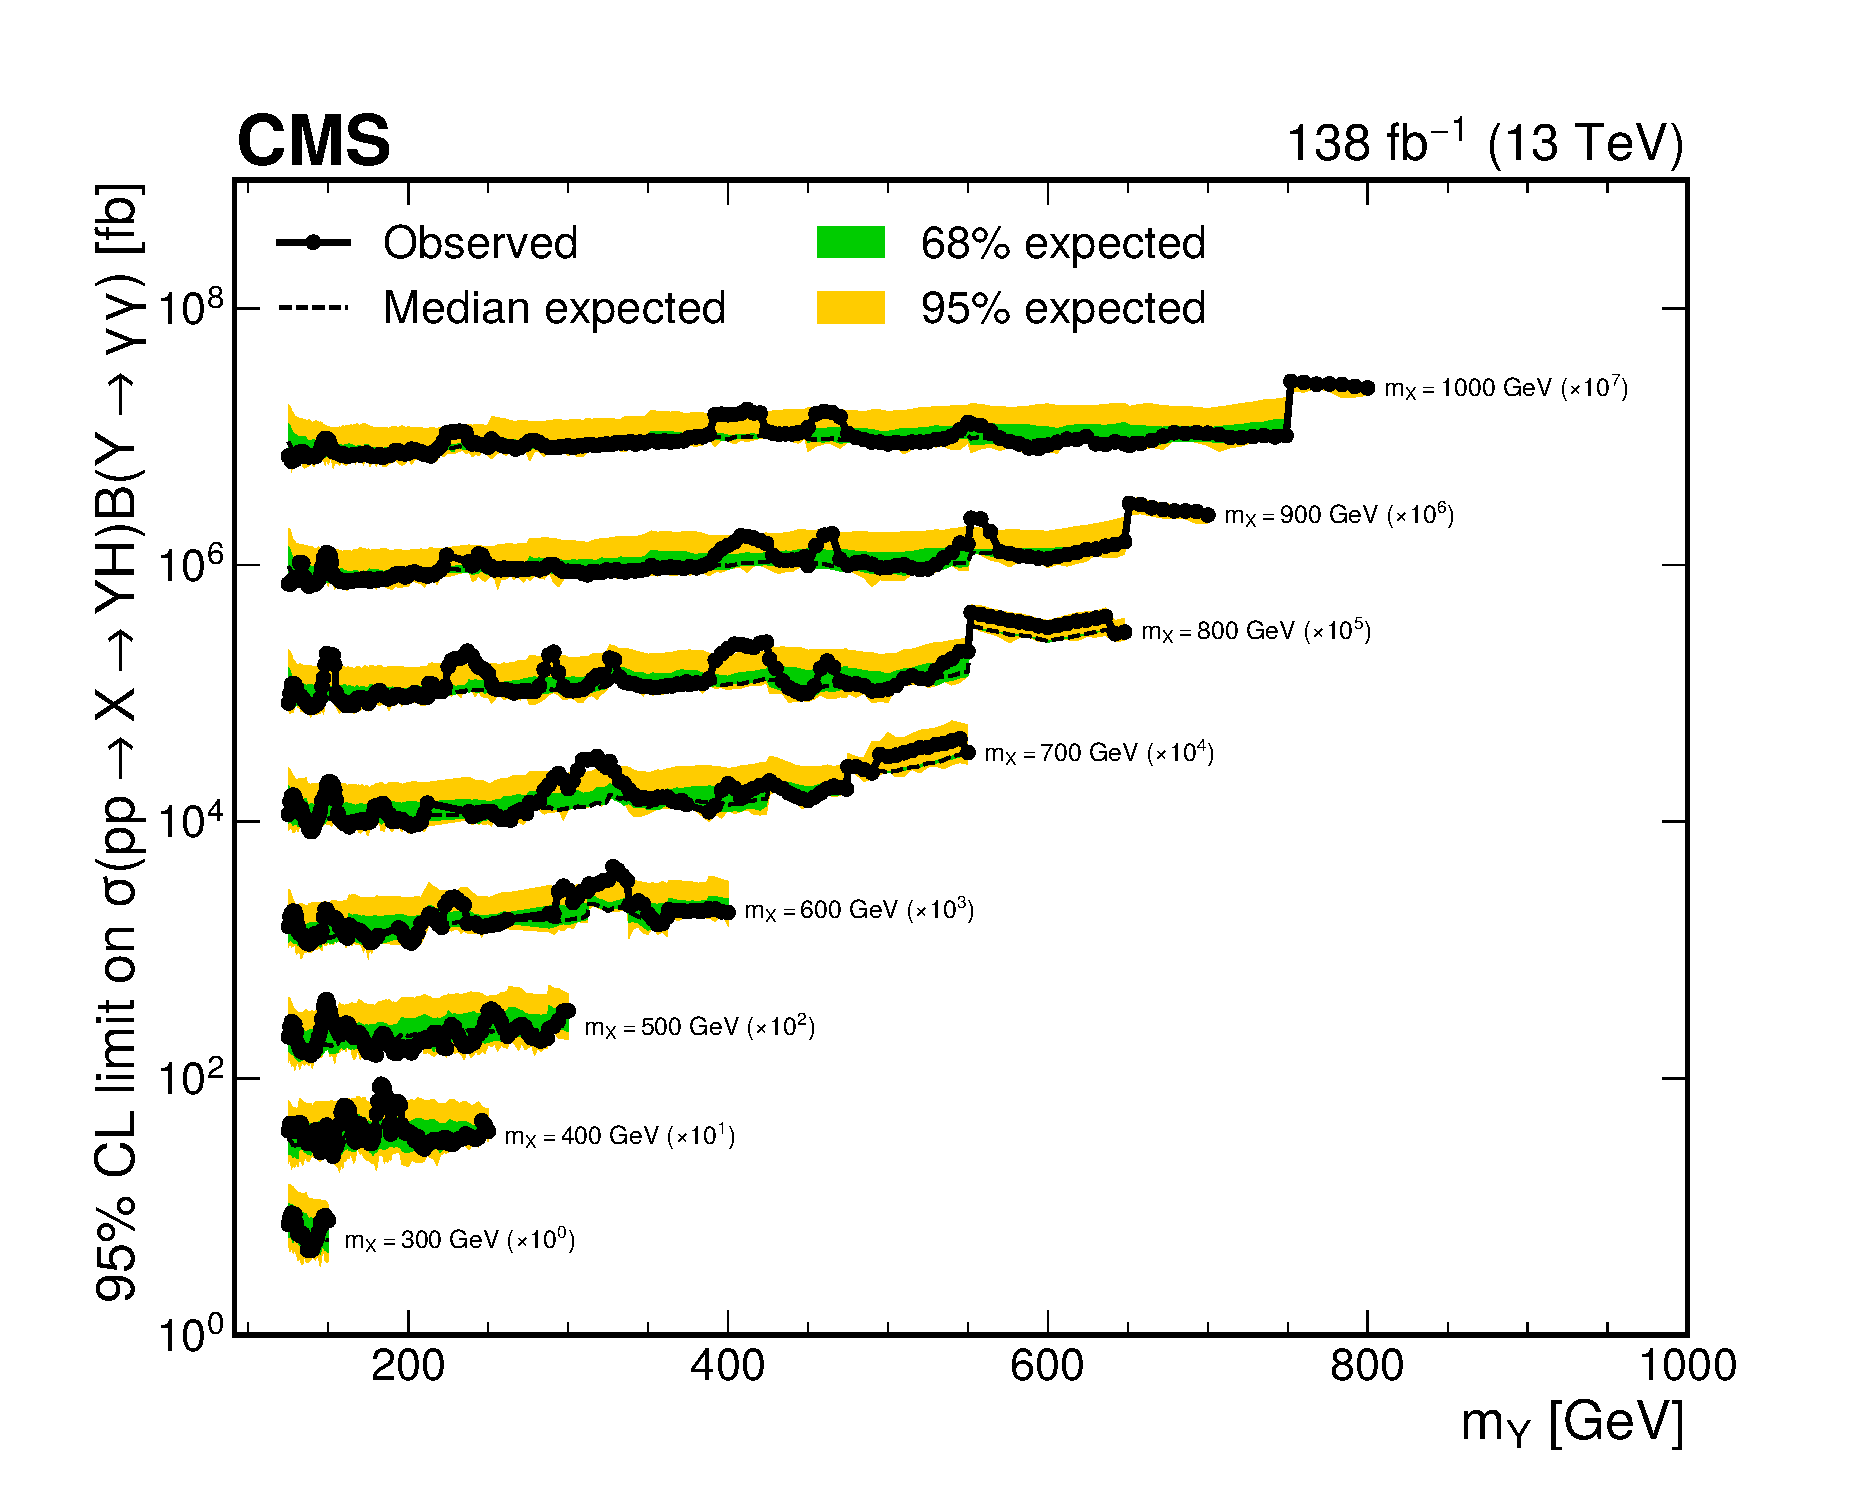
\includegraphics[width=\textwidth]{Figures/Dihiggs/results/limits/limits_stack_mx_y_gg_high_mass_paper.pdf}
    \caption[High-Mass \XYggHtt Upper Limits in as Function of \mY in Slices of \mX]{Expected and observed 95\% CL upper limits on $\sigma(\ppXYH)\BR(\Ygg)$ for the high-mass \XYggHtt search. Limits are shown as a function of \mY for the nominal values of \mX where the limits are scaled by orders of 10 as labelled in the plot. The solid and dashed black lines represent observed and median expected limits respectively. The inner (green) band and the outer (yellow) band indicate the regions containing 68 and 95\%, respectively, of the distribution of limits expected under the background-only hypothesis.}\label{fig:limits_stack_mx_y_gg_high_mass}
\end{figure}

\begin{figure}
    \centering
    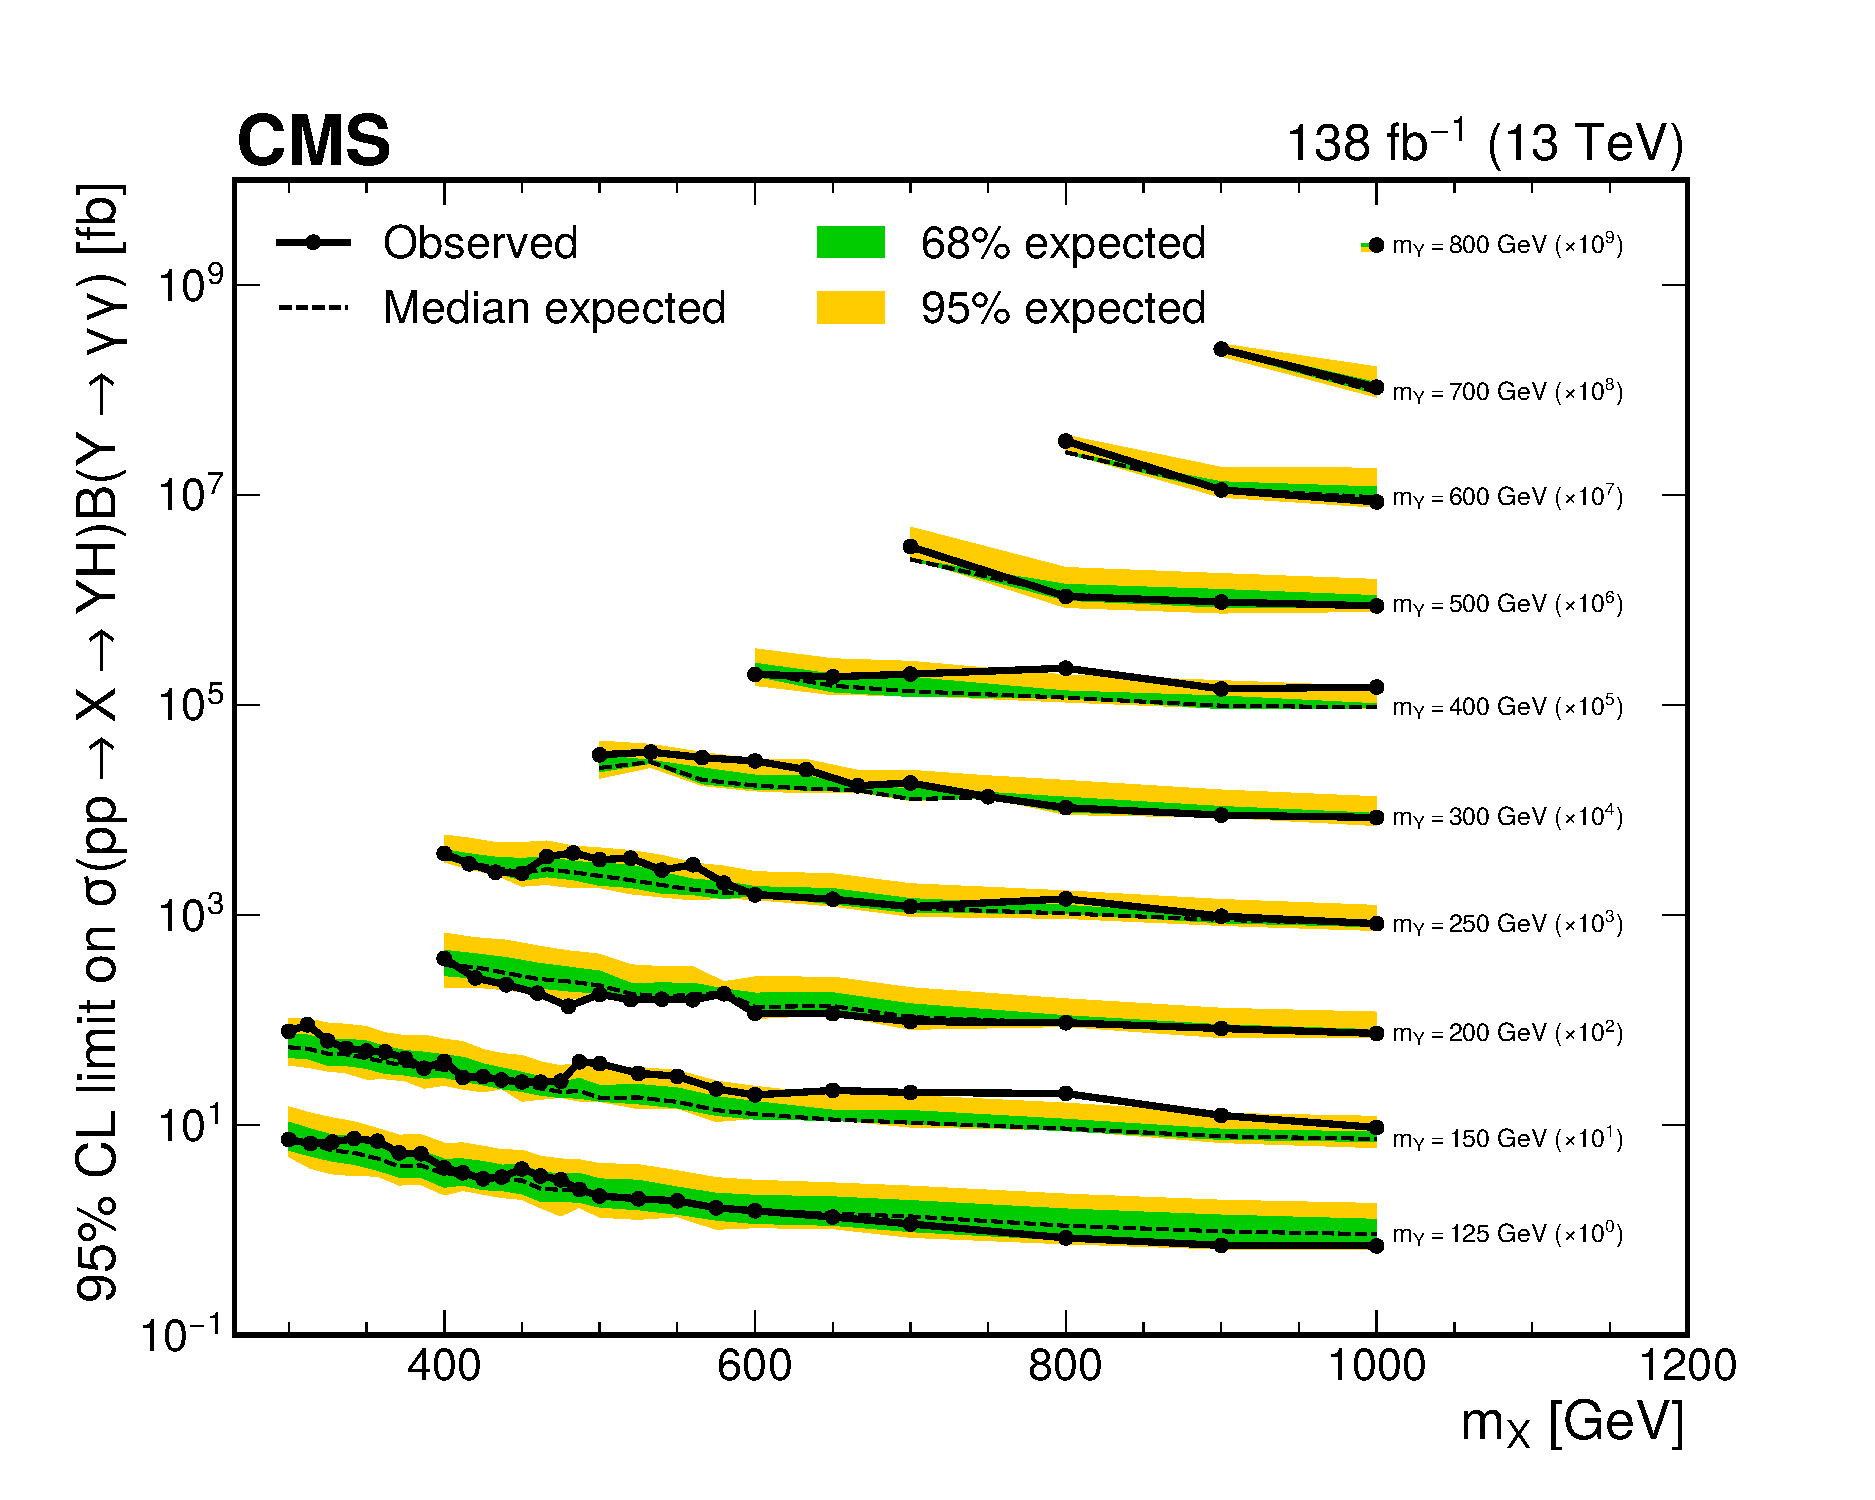
\includegraphics[width=\textwidth]{Figures/Dihiggs/results/limits/limits_stack_my_y_gg_high_mass_paper.pdf}
    \caption[High-Mass \XYggHtt Upper Limits in as Function of \mX in Slices of \mY]{Expected and observed 95\% CL upper limits on $\sigma(\ppXYH)\BR(\Ygg)$ for the high-mass \XYggHtt search. Limits are shown as a function of \mX for the nominal values of \mY where the limits are scaled by orders of 10 as labelled in the plot. The solid and dashed black lines represent observed and median expected limits respectively. The inner (green) band and the outer (yellow) band indicate the regions containing 68 and 95\%, respectively, of the distribution of limits expected under the background-only hypothesis.}\label{fig:limits_stack_my_y_gg_high_mass}
\end{figure}